\documentclass[14pt]{extarticle}

\usepackage[table]{xcolor}
\usepackage[normalem]{ulem} % strike through text
\usepackage{amsmath,mathtools,amsfonts,amsthm,amssymb,hyperref,wasysym,pifont}
\usepackage{parskip,geometry,latexsym,bookmark,mathtools,float,cancel,tcolorbox}

\newtheorem{defn}{Definition}
\newtheorem{thm}{Theorem}
\newtheorem{claim}{Claim}
\newtheorem{lemma}{Lemma}

\newcommand{\dps}{\displaystyle}
\newcommand{\fbl}{\underline{\hspace{1cm}}\,\,}
\newcommand{\R}{\mathbb{R}}
\newcommand{\Z}{\mathbb{Z}}
\newcommand{\from}{\leftarrow}
\newcommand{\true}{{\bf t}}
\newcommand{\false}{{\bf c}}
\newcommand{\bic}{\leftrightarrow}
\newcommand{\da}{\downarrow}
\newcommand{\fa}{\forall}
\newcommand{\te}{\exists}
\newcommand{\cy}{\color{cyan}}

\newcommand{\base}[1]{{\cy #1}} % for log bases
\newcommand{\floor}[1]{{\left\lfloor#1\right\rfloor}}
\newcommand{\ceil}[1]{{\left\lceil#1\right\rceil}}
\newcommand\Ccancel[2][black]{\renewcommand\CancelColor{\color{#1}}\cancel{#2}}
\newcommand\Cbcancel[2][black]{\renewcommand\CancelColor{\color{#1}}\bcancel{#2}}

\hypersetup{colorlinks,allcolors=blue,linktoc=all}
\geometry{a4paper}
\geometry{margin=0.42in}

\title{Chapter 4 Solutions, Susanna Epp Discrete Math 5th Edition}

\author{https://github.com/spamegg1}

\begin{document}
\maketitle
\tableofcontents

\section{Exercise Set 4.1}

\subsection{Exercise 1}
Assume that $k$ is a particular integer.

\subsubsection{(a)}
Is $-17$ an odd integer?

\begin{proof}
Yes: $-17 = 2(-9) + 1$.

\end{proof}

\subsubsection{(b)}
Is 0 neither even nor odd?

\begin{proof}
No. 0 is even because $0 = 0 \cdot 2$.
\end{proof}

\subsubsection{(c)}
Is $2k - 1$ odd?

\begin{proof}
Yes: $2k - 1 = 2(k - 1) + 1$ and $k - 1$ is an integer because it is a difference of integers.
\end{proof}

\subsection{Exercise 2}
Assume that $c$ is a particular integer.

\subsubsection{(a)}
Is $-6c$ an even integer?

\begin{proof}
Yes, because $-6c = 2 \cdot (-3c) = 2k$ where $k = -3c$ is an integer.
\end{proof}

\subsubsection{(b)}
Is $8c + 5$ an odd integer?

\begin{proof}
Yes, because $8c + 5 = 2(4c + 2) + 1$ and $k = 4k+2$ is an integer.
\end{proof}

\subsubsection{(c)}
Is $(c^2 + 1) - (c^2 - 1) - 2$ an even integer?

\begin{proof}
Yes, because it equals 0: $(c^2 + 1) - (c^2 - 1) - 2 = c^2 + 1 - c^2 + 1 - 2 = 2 - 2 = 0$.
\end{proof}

\subsection{Exercise 3}
Assume that $m$ and $n$ are particular integers.

\subsubsection{(a)}
Is $6m + 8n$ even?

\begin{proof}
Yes: $6m + 8n = 2(3m + 4n)$ and $(3m + 4n)$ is an integer because $3, 4, m$, and $n$ are integers, and products and sums of integers are integers.
\end{proof}

\subsubsection{(b)}
Is $10mn + 7$ odd?

\begin{proof}
Yes: $10mn + 7 = 2(5mn + 3) + 1$ and $5mn + 3$ is an integer because $3, 5, m$, and $n$ are integers, and products and sums of integers are integers.
\end{proof}

\subsubsection{(c)}
If $m > n > 0$, is $m^2 - n^2$ composite?

\begin{proof}
Not necessarily. For instance, if $m = 3$ and $n = 2$, then $m^2 - n^2 = 9 - 4 = 5$, which is prime. (However, $m^2 - n^2$ is composite for many values of $m$ and $n$ because of the identity $m^2 - n^2 = (m - n)(m + n)$.)
\end{proof}

\subsection{Exercise 4}
Assume that $r$ and $s$ are particular integers.

\subsubsection{(a)}
Is $4rs$ even?

\begin{proof}
Yes: $4rs = 2(2rs)$ and $2rs$ is an integer because $2, r, s$ are integers, and products of integers are integers.
\end{proof}

\subsubsection{(b)}
Is $6r + 4s^2 + 3$ odd?

\begin{proof}
Yes: $6r + 4s^2 + 3 = 2(3r + 2s^2 + 1) + 1$ and $3r + 2s^2 + 1$ is an integer because $3, r, 2, s, 1$ are integers and products and sums of integers are integers.
\end{proof}

\subsubsection{(c)}
If $r$ and $s$ are both positive, is $r^2 + 2rs + s^2$ composite?

\begin{proof}
Yes: $r^2 + 2rs + s^2 = (r+s)(r+s)$ and $r + s \geq 2$, therefore $r^2 + 2rs + s^2$ is a product of two integers both of which are greater than 1.
\end{proof}

{\bf \cy Prove the statements in 5–11.}

\subsection{Exercise 5}
There are integers $m$ and $n$ such that $m > 1$ and $n > 1$ and $\frac{1}{m} + \frac{1}{n}$ is an integer.

\begin{proof}
For example, let $m = n = 2$. Then $m$ and $n$ are integers such that $m > 1$ and $n > 1$ and $\frac{1}{m} + \frac{1}{n} = \frac{1}{2} + \frac{1}{2} = 1$ which is an integer.
\end{proof}

\subsection{Exercise 6}
There are distinct integers $m$ and $n$ such that $\frac{1}{m} + \frac{1}{n}$ is an integer.

\begin{proof}
For example, let $m = 1, n = -1$. Then $m$ and $n$ are integers such that $\frac{1}{m} + \frac{1}{n} = \frac{1}{1} - \frac{1}{1} = 0$ which is an integer.
\end{proof}

\subsection{Exercise 7}
There are real numbers $a$ and $b$ such that $\sqrt{a+b} = \sqrt{a} \sqrt{b}$.

\begin{proof}
For example, let $a = 0, b = 0$. Then $a$ and $b$ are real numbers such that 

$\sqrt{a+b} = \sqrt{0+0} = 0 = \sqrt{0} + \sqrt{0} = \sqrt{a} + \sqrt{b}$.
\end{proof}

\subsection{Exercise 8}
There is an integer $n > 5$ such that $2^n - 1$ is prime.

\begin{proof}
For example, let $n = 7$. Then $n$ is an integer such that
$n > 5$ and $2^n - 1 = 127$, which is prime.
\end{proof}

\subsection{Exercise 9}
There is a real number $x$ such that $x > 1$ and $2^x > x^{10}$.

\begin{proof}
For example, take $x = 80$. Then 

$x^{10} = 80^{10} = 8^{10} \cdot 10^{10} = (2^3)^{10} \cdot 10^{10} = 2^{30} \cdot 10^{10}$.

We have $2^{50} \approx 1,125899907 \cdot 10^{15} > 10^{10}$. So $2^{80} = 2^{30} \cdot 2^{50} > 2^{30} \cdot 10^{10} = 80^{10}$.

Therefore $x = 80$ is a real number such that $x > 1$ and $2^x > x^{10}$.
\end{proof}

\begin{tcolorbox}[colframe=cyan]
{\bf \cy Definition:} An integer $n$ is called a {\bf perfect square} if, and only if, $n = k^2$ for some integer $k$.
\end{tcolorbox}

\subsection{Exercise 10}
There is a perfect square that can be written as the sum of two other perfect squares.

\begin{proof}
For example, 25, 9, and 16 are all perfect squares, because $25 = 5^2, 9 = 3^2$, and $16 = 4^2$, and $25 = 9 + 16$. Thus 25 is a perfect square that can be written as a sum of two other perfect squares.
\end{proof}

\subsection{Exercise 11}
There is an integer $n$ such that $2n^2 - 5n + 2$ is prime.

\begin{proof}
For example, take $n = 3$. Then $2n^2 - 5n + 2 = 18 - 15 + 2 = 5$ is prime. (You can find this value of $n$ by either starting at $n = 1$ and using trial and error, or noticing that $2n^2 - 5n + 2 = (2n - 1)(n - 2)$, so, for this to be prime, one of the factors has to be 1.)
\end{proof}

{\bf \cy In $12-13$, (a) write a negation for the given statement, and (b) use a counterexample to disprove the given statement. explain how the counterexample actually shows that the given statement is false.}

\subsection{Exercise 12}
For all real numbers $a$ and $b$, if $a < b$ then $a^2 < b^2$.

\begin{proof}
a. {\it Negation for the statement:} There exist real numbers $a$ and $b$ such that $a < b$ and $a^2 \nless b^2$.

b. {\it Counterexample for the statement:} Let $a = -2$ and
$b = -1$. Then $a < b$ because $-2 < -1$, but $a^2 \nless b^2$ because $(-2)^2 = 4$ and $(-1)^2 = 1$ and $4 \nless 1$. {\it [So the hypothesis of the statement is true and its conclusion is false.]}
\end{proof}

\subsection{Exercise 13}
For every integer $n$, if $n$ is odd then $\frac{n-1}{2}$ is odd.

\begin{proof}
a. {\it Negation for the statement:} There exists an integer $n$ such that $n$ is odd and $\frac{n-1}{2}$ is not odd.

b. {\it Counterexample for the statement:} Let $n = 5$. Then $n$ is odd because $5 = 2 \cdot 2 + 1$, but $\frac{n-1}{2}$ is not odd because $\frac{5-1}{2} = 2 = 2 \cdot 1$ is even. {\it [So the hypothesis of the statement is true and its conclusion is false.]}
\end{proof}

{\bf \cy Disprove each of the statements in $14-16$ by giving a counterexample. In each case explain how the counterexample actually disproves the statement.}

\subsection{Exercise 14}
For all integers $m$ and $n$, if $2m + n$ is odd then $m$ and $n$ are both odd.

\begin{proof}
\underline{Counterexample:} Let $m = 2$ and $n = 1$. Then $2m + n = 2 \cdot 2 + 1 = 5$, which is odd. But $m$ is not odd, and so it is false that both $m$ and $n$ are odd. {\it [This is one counterexample among many.]}
\end{proof}

\subsection{Exercise 15}
For every integer $p$, if $p$ is prime then $p^2 - 1$ is even.

\begin{proof}
\underline{Counterexample:} Let $p = 2$ which is prime, but $p^2 - 1 = 2^2 - 1 = 4 - 1 = 3$ is not even. {\it [This is the only counterexample! For every other prime $p$, $p^2 - 1$ is even.]}
\end{proof}

\subsection{Exercise 16}
For every integer $n$, if $n$ is even then $n^2 + 1$ is prime.

\begin{proof}
\underline{Counterexample:} Let $n = 8$. Then $n$ is even. But $n^2 + 1 = 65 = 13 \cdot 5$ is not prime. {\it [This is one counterexample among many.]}
\end{proof}

{\bf \cy In $17-20$, determine whether the property is true for all integers, true for no integers, or true for some integers and false for other integers. Justify your answers.}

\subsection{Exercise 17}
$(a+b)^2 = a^2 + b^2$

\begin{proof}
This property is true for some integers and false for other integers. For instance, if $a = 0$ and $b = 1$, the property is true because $(0 + 1)^2 = 0^2 + 1^2$, but if $a = 1$ and $b = 1$, the property is false because $(1 + 1)^2 = 4$ and $1^2 + 1^2 = 2$ and $4 \neq 2$.
\end{proof}

\subsection{Exercise 18}
$\dps \frac{a}{b} + \frac{c}{d} = \frac{a+c}{b+d}$

\begin{proof}
True for some integers, false for others. For example, if $a = c = 0$ and $b = d = 1$ then $\dps \frac{0}{1} + \frac{0}{1} = 0 = \frac{0+0}{1+1}$ is true. But if $a = 1, b = 2, c = 3$ and $d = 4$ then 

$\dps \frac{a}{b} + \frac{c}{d} = \frac{1}{2} + \frac{3}{4} = \frac{5}{4} \neq \frac{4}{6} = \frac{1+3}{2+4} = \frac{a+c}{b+d}$.
\end{proof}

\subsection{Exercise 19}
$-a^n = (-a)^n$

{\it Hint:} This property is true for some integers and false for other integers. To justify this answer you need to find examples of both.

\begin{proof}
True for some integers: let $a = 0, n = 1$. Then $-0^1 = -0 = 0$ and $(-0)^1 = 0^1 = 0$ so the equality holds. When $a = n = 2$ it is false: $-2^2 = -4$ but $(-2)^2 = 4$ and $-4 \neq 4$.
\end{proof}

\subsection{Exercise 20}
The average of any two odd integers is odd.

\begin{proof}
True for some, false for others. For example, 3 and 7 are both odd, and their average $(3+7)/2 = 5$ is odd. But 3 and 5 are both odd, and their average is $(3 + 5) / 2 = 4$ is even.
\end{proof}

{\bf \cy Prove the statement in 21 and 22 by the method of exhaustion.}

\subsection{Exercise 21}
Every positive even integer less than 26 can be expressed as a sum of three of fewer perfect squares. (For instance, $10 = 1^2 + 3^2$ and $16 = 4^2$.)

\begin{proof}
$2 = 1^2 + 1^2$

$4 = 2^2$

$6 = 2^2 + 1^2 + 1^2$

$8 = 2^2 + 2^2$

$10 = 1^2 + 3^2$

$12 = 2^2 + 2^2 + 2^2$

$16 = 4^2$

$18 = 4^2 + 1^2 + 1^2$

$20 = 4^2 + 2^2$

$22 = 2^2 + 2^2 + 3^2$

$24 = 4^2 + 2^2 + 2^2$
\end{proof}

\subsection{Exercise 22}
For each integer $n$ with $1 \leq n \leq 10$, $n^2 - n + 11$ is a prime number.

\begin{proof}
$1^2 - 1 + 11 = 11$ is prime.

$2^2 - 2 + 11 = 13$ is prime.

$3^2 - 3 + 11 = 17$ is prime.

$4^2 - 4 + 11 = 23$ is prime.

$5^2 - 5 + 11 = 31$ is prime.

$6^2 - 6 + 11 = 41$ is prime.

$7^2 - 7 + 11 = 53$ is prime.

$8^2 - 8 + 11 = 67$ is prime.

$9^2 - 9 + 11 = 83$ is prime.

$10^2 - 10 + 11 = 101$ is prime.
\end{proof}

{\bf \cy Each of the statements in $23-26$ is true. For each, (a) rewrite the statement with the quantification implicit as If \fbl, then \fbl, and (b) write the first sentence of a proof (the “starting point”) and the last sentence of a proof (the “conclusion to be shown”). (Note that you do not need to understand the statements in order to be able to do these exercises.)}

\subsection{Exercise 23}
For every integer $m$, if $m > 1$ then $0 < \frac{1}{m} < 1$.

\begin{proof}
a. If an integer is greater than 1, then its reciprocal is
between 0 and 1.

b. {\it Start of proof:} Suppose $m$ is any integer such that $m > 1$. {\it Conclusion to be shown:} $0 < 1/m < 1$.
\end{proof}

\subsection{Exercise 24}
For every real number $x$, if $x > 1$ then $x^2 > x$.

\begin{proof}
a. If a real number is greater than 1, then its square is greater than itself.

b. {\it Start of proof:} Suppose $x$ is any real number such that $x > 1$. {\it Conclusion to be shown:} $x^2 > x$.
\end{proof}

\subsection{Exercise 25}
For all integers $m$ and $n$, if $mn = 1$ then $m = n = 1$ or $m = n = -1$.

\begin{proof}
a. If the product of two integers is 1, then either both are 1 or both are $-1$.

b. {\it Start of proof:} Suppose $m$ and $n$ are any integers with $mn = 1$. {\it Conclusion to be shown:} $m = n = 1$ or $m = n = -1$.
\end{proof}

\subsection{Exercise 26}
For every real number $x$, if $0 < x < 1$ then $x^2 < x$.

\begin{proof}
a. If a real number is strictly between 0 and 1, then its square is less than itself.

b. {\it Start of proof:} Suppose $x$ is any real number such that $0 < x < 1$. {\it Conclusion to be shown:} $x^2 < x$.
\end{proof}

\subsection{Exercise 27}
Fill in the blanks in the following proof.

{\bf Theorem:} For every odd integer $n$, $n^2$ is odd.

{\bf Proof:} Suppose $n$ is any {\cy (a)} \fbl. By definition of odd, $n = 2k + 1$ for some integer $k$. Then

\begin{center}
\begin{tabular}{rcll}
$n^2$ & = & {\cy (b)} $(\fbl)^2$ & \cy by substitution \\
& = & $4k^2 + 4k + 1$ & \cy by multiplying \\
& = & $2(2k^2 + 2k) + 1$ & \cy by factoring out a 2 \\
\end{tabular}
\end{center}

Now $2k^2 + 2k$ is an integer because it is a sum of products of integers. Therefore, $n^2$ equals $2\cdot$ (an integer) $+ 1$, and so {\cy (c)} \fbl is odd by definition of odd.

Because we have not assumed anything about $n$ except that it is an odd integer, it follows from the principle of {\cy (d)} \fbl that for every odd integer $n$, $n^2$ is odd.

\begin{proof}
(a) particular but arbitrarily chosen odd integer 
(b) $2k + 1$ (c) $n^2$ (d) universal generalization
\end{proof}

{\bf \cy In each of $28-31$: \\ 
a. Rewrite the theorem in three different ways: as $\fa$ \fbl, if \fbl, then \fbl; as $\fa$ \fbl, \fbl (without using the words if or then), and as If \fbl, then \fbl (without using an explicit universal quantifier). \\
b. Fill in the blanks in the proof of the theorem.}

\subsection{Exercise 28}
{\bf Theorem:} The sum of any two odd integers is even.

{\bf Proof:} Suppose $m$ and $n$ are any {\it [particular but arbitrarily chosen]} odd integers. 

{\it [We must show that $m + n$ is even.]}

By {\cy (a)} \fbl, $m = 2r + 1$ and $n = 2s + 1$ for some integers $r$ and $s$. Then

\begin{center}
\begin{tabular}{rcll}
$m+n$ & = & $(2r+1) + (2s+1)$ & {\cy by (b)} \fbl \\
& = & $2r + 2s + 2$ & \\
& = & $2(r+s+1)$ & \cy by algebra \\
\end{tabular}
\end{center}

Let $u = r + s + 1$. Then $u$ is an integer because $r, s$ and 1 are integers and because {\cy (c)} \fbl. 

Hence $m + n = 2u$, where $u$ is an integer, and so, by {\cy (d)} \fbl, $m + n$ is even {\it [as was to be shown]}.

\begin{proof}
a. $\fa$ integers $m$ and $n$, if $m$ and $n$ are odd then $m + n$ is even.

$\fa$ odd integers $m$ and $n$, $m + n$ is even.

If $m$ and $n$ are any odd integers, then $m + n$ is even.

b. (a) definition of odd, (b) substitution, (c) any sum of
integers is an integer, (d) definition of even
\end{proof}

\subsection{Exercise 29}
{\bf Theorem:} The negative of any even integer is even.

{\bf Proof:} Suppose $n$ is any {\it [particular but arbitrarily chosen]} even integer. 

{\it [We must show that $-n$ is even.]}

By {\cy (a)} \fbl, $n = 2k$ for some integer $k$.

Then

\begin{center}
\begin{tabular}{rcll}
$-n$ & = & $-(2k)$ & \cy by (b) \fbl \\
& = & $2(-k)$ & \cy by algebra \\
\end{tabular}
\end{center}

Let $r = -k$. Then $r$ is an integer because $-1$ and $k$ are integers and {\cy (c)} \fbl. 

Hence $-n = 2r$, where $r$ is an integer, and so $-n$ is even by {\cy (d)} \fbl {\it [as was to be shown]}.

\begin{proof}
a. $\fa$ integer $n$, if $n$ is even then $-n$ is even.

$\fa$ even integer $n$, $-n$ is even.

If $n$ is any even integer, then $-n$ is even.

b. (a) definition of even, (b) substitution, (c) any product of integers is an integer, (d) definition of even
\end{proof}

\subsection{Exercise 30}
{\bf Theorem:} The sum of any even integer and any odd integer is odd.

{\bf Proof:} Suppose $m$ is any even integer and $n$ is any {\cy (a)} \fbl. By definition of even, $m = 2r$ for some {\cy (b)} \fbl, and by definition of odd, $n = 2s + 1$ for some integer $s$. By substitution and algebra,

\begin{center}
\begin{tabular}{ccccc}
$m+n$ & = & {\cy (c)} \fbl & = & $2(r+s)+1$ \\
\end{tabular}
\end{center}

Since $r$ and $s$ are integers, so is their sum $r+s$. Hence $m+n$ has the form twice some integer plus one, and so, by {\cy (d)} \fbl by definition of odd.

\begin{proof}
a. $\fa$ integers $m$ and $n$, if $m$ is even and $n$ is odd, then $m + n$ is odd.

$\fa$ even integers $m$ and odd integers $n$, $m + n$ is odd.

If $m$ is any even integer and $n$ is any odd integer,
then $m + n$ is odd.

b. (a) any odd integer (b) integer $r$ (c) $2r + (2s + 1)$ (d) $m + n$ is odd
\end{proof}

\subsection{Exercise 31}
{\bf Theorem:} Whenever $n$ is an odd integer, $5n^2 + 7$ is even.

{\bf Proof:} Suppose $n$ is any {\it [particular but arbitrarily chosen]} odd integer. 

{\it [We must show that $5n^2 + 7$ is even.]}

By definition of odd, $n = $ {\cy (a)} \fbl, for some integer $k$. 

Then

\begin{center}
\begin{tabular}{rcll}
$5n^2 + 7$ & = & {\cy (b)} \fbl & \cy substitution \\
& = & $5(4k^2 + 4k + 1) + 7$ & \\
& = & $20k^2 + 20k + 12$ & \\
& = & $2(10k^2 + 10k + 6)$ & \cy by algebra \\
\end{tabular}
\end{center}

Let $t = $ {\cy (c)} \fbl. Then $t$ is an integer because products and sums of integers are integers. 

Hence $5n^2 + 7 = 2t$, where $t$ is an integer, and thus {\cy (d)} \fbl by definition of even {\it [as was to be shown]}.

\begin{proof}
a. $\fa$ integer $n$, if $n$ is odd, then $5n^2+7$ is even.

$\fa$ odd integer $n$, $5n^2+7$ is even.

If $n$ is any odd integer, then $5n^2+7$ is even.

b. (a) $2k+1$ (b) $5(2k+1)^2 + 7$ (c) $10k^2 + 10k + 6$ (d) $5n^2+7$ is even
\end{proof}

\section{Exercise Set 4.2}

{\bf \cy Prove the statements in $1-11$. In each case use only the definitions of the terms and the assumptions listed on page 161, not any previously established properties of odd and even integers. Follow the directions given in this section for writing proofs of universal statements.}

\subsection{Exercise 1}
For every integer $n$, if $n$ is odd then $3n + 5$ is even.

\begin{proof}
Suppose $n$ is any {\it [particular but arbitrarily chosen]} odd integer. 

{\it [We must show that $3n + 5$ is even. By definition of even, this means we must show that $3n + 5 = 2\cdot$(some integer).]}

By definition of odd, $n = 2r + 1$, for some integer $r$. 

Then

\begin{center}
\begin{tabular}{rcll}
$3n + 5$ & = & $3(2r + 1) + 5$ & \cy by substitution \\
& = & $6r + 3 + 5$ & \\
& = & $6r + 8$ & \\
& = & $2(3r + 4)$ & \cy by algebra \\
\end{tabular}
\end{center}

{\it [Idea for the rest of the proof: We want to show that $3n + 5 = 2\cdot$(some integer). At this point we know that $3n + 5 = 2(3r + 4)$. So is $3r + 4$ an integer? Yes, because products and sums of integers are integers.]}

Let $k = 3r + 4$. 

Then $k$ is an integer because products and sums of integers are integers. 

Hence $3n + 5 = 2(3r+4) = 2k$ where $k$ is an integer. Hence by definition of even $3n+5$ is even {\it [as was to be shown]}.
\end{proof}

\subsection{Exercise 2}
For every integer $m$, if $m$ is even then $3m + 5$ is odd.

\begin{proof}
Suppose $m$ is any {\it [particular but arbitrarily chosen]} even integer. 

{\it [We must show that $3m + 5$ is odd. By definition of odd, this means we must show that $3m + 5 = 2\cdot\text{(some integer)} + 1$.]}

By definition of even, $m = 2r$, for some integer $r$. 

Then

\begin{center}
\begin{tabular}{rcll}
$3m + 5$ & = & $3(2r) + 5$ & \cy by substitution \\
& = & $6r + 5$ & \\
& = & $6r + 4 + 1$ & \\
& = & $2(3r + 2) + 1$ & \cy by algebra \\
\end{tabular}
\end{center}

{\it [Idea for the rest of the proof: We want to show that $3m + 5 = 2\cdot\text{(some integer)} + 1$. At this point we know that $3m + 5 = 2(3r + 2) + 1$. So is $3r + 2$ an integer? Yes, because products and sums of integers are integers.]}

Let $k = 3r + 2$. 

Then $k$ is an integer because products and sums of integers are integers. 

Hence $3m + 5 = 2(3r+2) + 1 = 2k + 1$ where $k$ is an integer. Hence by definition of odd $3n+5$ is odd {\it [as was to be shown]}.
\end{proof}

\subsection{Exercise 3}
For every integer $n$, $2n - 1$ is odd.

\begin{proof}
Suppose $n$ is any {\it [particular but arbitrarily chosen]} integer. 

{\it [We must show that $2n - 1$ is odd. By definition of odd, this means we must show that $2n - 1 = 2 \cdot \text{(some integer)} + 1$.]}

Then

\begin{center}
\begin{tabular}{rcll}
$2n-1$ & = & $2n - 2 + 2 - 1$ & \cy because $-2 + 2 = 0$ \\
& = & $2(n-1) + 2 - 1$ & \\
& = & $2(n-1) + 1$ & \cy by algebra \\
\end{tabular}
\end{center}

Let $k = n-1$. 

Then $k$ is an integer because the difference of two integers ($n$ and $1$) is an integer. 

Hence $2n-1 = 2(n-1) + 1 = 2k + 1$ where $k$ is an integer, and thus by definition of odd $2n-1$ is odd {\it [as was to be shown]}.
\end{proof}

\subsection{Exercise 4}
The difference of any even integer minus any odd integer is odd.

\begin{proof}
Suppose $a$ is any even integer and $b$ is any odd integer. 
{\it [We must show that $a - b$ is odd.]} By definition of even and odd, $a = 2r$ and $b = 2s + 1$, for some integers $r, s$. By substitution and algebra,
\[
a-b = 2r - (2s+1) = 2r-2s-1 = 2r-2s-2+2-1 = 2(r-s-1)+1
\]
Let $t = r-s-1$. Then $t$ is an integer because differences of integers are integers. 

Thus $a-b = 2t+1$ where $t$ is an integer, and so by definition of odd $a-b$ is odd {\it [as was to be shown]}.
\end{proof}

\subsection{Exercise 5}
If $a$ and $b$ are any odd integers, then $a^2 + b^2$ is even.

\begin{proof}
Suppose $a,b$ are any {\it [particular but arbitrarily chosen]} odd integers. 

{\it [We must show that $a^2+b^2$ is even.]}

By definition of odd, $a = 2r+1$ and $b = 2s+1$, for some integers $r,s$. 

Then

\begin{center}
\begin{tabular}{rcll}
$a^2+b^2$ & = & $(2r+1)^2 + (2s+1)^2$ & \cy by substitution \\
& = & $(4r^2 + 4r + 1) + (4s^2 + 4s + 1)$ & \cy by multiplying \\
& = & $4r^2 + 4r + 4s^2 + 4s + 2$ & \cy by adding \\
& = & $2(2r^2+2r+2s^2+2s+1)$ & \cy by factoring out \\
\end{tabular}
\end{center}

Let $k = 2r^2+2r+2s^2+2s+1$. 

Then $k$ is an integer because squares, products and sums of integers are integers. 

Hence $a^2+b^2 = 2k$ where $k$ is an integer, and thus by definition of even $a^2+b^2$ is even {\it [as was to be shown]}.
\end{proof}

\subsection{Exercise 6}
If $k$ is any odd integer and $m$ is any even integer, then $k^2 + m^2$ is odd.

\begin{proof}
Suppose $k$ is any odd integer and $m$ is any even integer. 

{\it [We must show that $k^2 + m^2$ is odd.]}

By definition of odd and even, $k = 2a+1$ and $m = 2b$, for some integers $a, b$. Then

\begin{center}
\begin{tabular}{rcll}
$k^2+m^2$ & = & $(2a+1)^2+(2b)^2$ & \cy by substitution \\
& = & $4a^2+4a+1+4b^2$ & \\
& = & $4(a^2+a+b^2)+1$ & \\
& = & $2(2a^2+2a+2b^2)+1$ & \cy by algebra \\
\end{tabular}
\end{center}

But $2a^2+2a+2b^2$ is an integer because it is a sum of products of integers. Thus $k^2+m^2$ is twice an integer plus 1, and so $k^2+m^2$ is odd {\it [as was to be shown]}.
\end{proof}

\subsection{Exercise 7}
The difference between the squares of any two consecutive integers is odd.

\begin{proof}
Suppose $m$ and $n$ are any {\it [particular but arbitrarily chosen]} two consecutive integers. 

{\it [We must show that $m^2-n^2$ (or $n^2-m^2$) is odd.]}

By definition of consecutive, $m = k$ and $n = k+1$, for some integer $k$. 

Then

\begin{center}
\begin{tabular}{rcll}
$m^2-n^2$ & = & $k^2 - (k+1)^2$ & \cy by substitution \\
& = & $k^2 - (k^2 + 2k + 1)$ & \\
& = & $k^2 - k^2 - 2k - 1$ & \\
& = & $-2k-1$ & \\
& = & $-2k-2+2-1$ & \\
& = & $2(-k-1)+1$ & \cy by algebra \\
\end{tabular}
\end{center}

Let $r = -k-1$. Then $r$ is an integer because it is a difference of integers. 

Hence $m^2 - n^2 = 2r+1$ where $r$ is an integer, and thus by definition of odd $m^2-n^2$ is odd {\it [as was to be shown]}.
\end{proof}

\subsection{Exercise 8}
For any integers $m$ and $n$, if $m$ is even and $n$ is odd
then $5m + 3n$ is odd.

\begin{proof}
Suppose $m$ is any even integer and $n$ is any odd integer.  

{\it [We must show that $5m+3n$ is odd.]}

By definition of even and odd, $m = 2r$ and $n = 2s+1$, for some integers $r, s$. 

Then

\begin{center}
\begin{tabular}{rcll}
$5m+3n$ & = & $5(2r)+3(2s+1)$ & \cy by substitution \\
& = & $10r+6s+3$ & \\
& = & $10r+6s+2+1$ & \\
& = & $2(5r+3s+1)+1$ & \cy by algebra \\
\end{tabular}
\end{center}

Let $k = 5r+3s+1$. 

Then $k$ is an integer because it is a sum of products of integers. 

Hence $5m+3n = 2k+1$ where $k$ is an integer, and thus by definition of odd $5m+3n$ is odd {\it [as was to be shown]}.
\end{proof}

\subsection{Exercise 9}
If an integer greater than 4 is a perfect square, then the immediately preceding integer is not prime.

\begin{proof}
Suppose $n$ is any integer greater than 4 that is a perfect square. 

{\it [We must show that $n-1$ is not prime, in other words, $n-1$ is composite.]}

By definition of perfect square, $n = k^2$, for some integer $k$. 

Without loss of generality, we may assume $k > 0$, because $n = k^2 = (-k)^2$, and if $k$ is negative, we can replace it with $-k$ which is positive.

Since $n > 4$ we have $n - 4 > 0$. So $k^2 - 4 > 0$. So $(k-2)(k+2) > 0$. So either $k-2$ and $k+2$ are both negative, or they are both positive. Since $k > 0$, $k+2>2>0$, so they have to be both positive. Therefore, $k - 2 > 0$ so $k > 2$.

Then

\begin{center}
\begin{tabular}{rcll}
$n-1$ & = & $k^2-1$ & \cy by substitution \\
& = & $(k-1)(k+1)$ & \cy by algebra \\
\end{tabular}
\end{center}

Since $k>2$ we have both $k-1>1$ and $k+1>3>1$.

Hence $n-1$ is a product of two positive integers both greater than 1, and thus by definition of composite $n-1$ is composite {\it [as was to be shown]}.
\end{proof}

\subsection{Exercise 10}
If $n$ is any even integer, then $(-1)^n = 1$.

\begin{proof}
Suppose $n$ is any even integer. {\it [We must show that $(-1)^n = 1$.]}

By definition of even, $n = 2k$, for some integer $k$. 

Then by the laws of exponents from algebra $(-1)^n = (-1)^{2k} = ((-1)^2)^k = 1^k = 1$, {\it [as was to be shown]}.
\end{proof}

\subsection{Exercise 11}
If $n$ is any odd integer, then $(-1)^n = -1$.

\begin{proof}
Suppose $n$ is any odd integer. {\it [We must show that $(-1)^n = -1$.]}

By definition of even, $n = 2k+1$, for some integer $k$. 

Then by the laws of exponents from algebra 
\[
(-1)^n = (-1)^{2k+1} = (-1)^{2k}\cdot(-1) = ((-1)^2)^k\cdot(-1) = 1^k\cdot(-1) = 1\cdot(-1) = -1
\] 
{\it [as was to be shown]}.
\end{proof}

{\bf \cy Prove that the statements in $12-14$ are false.}

\subsection{Exercise 12}
There exists an integer $m \geq 3$ such that $m^2 - 1$ is prime.

\begin{proof}
To prove the given statement is false, we prove that its
negation is true.

The negation of the statement is “For every integer $m \geq 3$, $m^2 - 1$ is not prime.”

{\it Proof of the negation:} Suppose $m$ is any integer with $m \geq 3$. 

By basic algebra, $m^2 - 1 = (m - 1)(m + 1)$. 

Because $m \geq 3$, both $m - 1$ and $m + 1$ are positive integers greater than 1, and each is smaller than $m^2 - 1$. 

So $m^2 - 1$ is a product of two smaller positive integers, each greater than 1, and hence $m^2 - 1$ is not prime.
\end{proof}

\subsection{Exercise 13}
There exists an integer $n$ such that $6n + 27$ is prime.

\begin{proof}
To prove the given statement is false, we prove that its
negation is true.

The negation of the statement is “For every integer $n$, $6n+27$ is not prime. In other words, $6n+27$ is composite.”

{\it Proof of the negation:} Suppose $n$ is any integer. 
By basic algebra, $6n + 27 = 3(2n + 9)$. 

Hence $6n+27$ is the product of two integers greater than 1. Therefore by definition of composite, $6n+27$ is composite.
\end{proof}

\subsection{Exercise 14}
There exists an integer $k \geq 4$ such that $2k^2 - 5k + 2$ is prime.

\begin{proof}
To prove the given statement is false, we prove that its
negation is true.

The negation of the statement is “For every integer $k \geq 4$, $2k^2 - 5k + 2$ is composite.”

{\it Proof of the negation:} Suppose $k$ is any integer. 

By basic algebra, $2k^2 - 5k + 2 = (2k-1)(k-2)$. 

Because $k \geq 4$, $2k - 1 \geq 7$ and $k - 2 \geq 2$. So both $2k-1$ and $k-2$ are integers greater than 1. 

Hence $2k^2 - 5k + 2$ is the product of two integers greater than 1. Therefore by definition of composite, $2k^2 - 5k + 2$ is composite.
\end{proof}

{\bf \cy Find the mistakes in the “proofs” shown in $15-19$.}

\subsection{Exercise 15}
{\bf Theorem:} For every integer $k$, if $k > 0$ then $k^2 + 2k + 1$ is composite.

“{\bf Proof:} For $k = 2$, $k > 0$ and $k^2 + 2k + 1 = 2^2 + 2\cdot2 + 1 = 9$. And since $9 = 3\cdot3$, then 9 is composite. Hence the theorem is true.”

\begin{proof}
The incorrect proof just shows the theorem to be true in
the one case where $k = 2$. A real proof must show that it
is true for {\it every} integer $k > 0$.
\end{proof}

\subsection{Exercise 16}
{\bf Theorem:} The difference between any odd integer and any even integer is odd.

“{\bf Proof:} Suppose $n$ is any odd integer, and $m$ is any even integer. By definition of odd, $n = 2k + 1$ where $k$ is an integer, and by definition of even, $m = 2k$ where $k$ is an integer. Then $n - m = (2k + 1) - 2k = 1$, and 1 is odd. Therefore, the difference between any odd integer and any even integer is odd.”

\begin{proof}
The mistake in the “proof” is that the same symbol, $k$, is used to represent two different quantities. By setting $m = 2k$ and $n = 2k + 1$, the proof implies that $n = m + 1$, and thus it deduces the conclusion only for this one situation. When $m = 4$ and $n = 17$, for instance, the computations in the proof indicate that $n - m = 1$, but actually $n - m = 13$. In other words, the proof does not deduce the conclusion for an arbitrarily chosen even integer $m$ and odd integer $n$, and hence it is invalid.
\end{proof}

\subsection{Exercise 17}
{\bf Theorem:} For every integer $k$, if $k > 0$ then $k^2 + 2k + 1$ is composite.

{\bf Proof:} Suppose $k$ is any integer such that $k > 0$. If $k^2 + 2k + 1$ is composite, then $k^2 + 2k + 1 = rs$
for some integers $r$ and $s$ such that 

$1 < r < k^2 + 2k + 1$ and $1 < s < k^2 + 2k + 1$.

Since $k^2 + 2k + 1 = rs$ and both $r$ and $s$ are strictly between 1 and $k^2 + 2k + 1$, then $k^2 + 2k + 1$ is not prime. So $k^2 + 2k + 1$ is composite as was to be shown.

\begin{proof}
This incorrect proof assumes what is to be proved. The word since in the third sentence is completely unjustified. The second sentence tells only what happens if $k^2 + 2k = 1$ is composite. But at that point in the proof, it has not been established that $k^2 + 2k + 1$ is composite. In fact, that is exactly what is to be proved.
\end{proof}

\subsection{Exercise 18}
{\bf Theorem:} The product of any even integer and any odd integer is even.

“{\bf Proof:} Suppose $m$ is any even integer and $n$ is any odd integer. If $m\cdot n$ is even, then by definition of even there exists an integer $r$ such that $m\cdot n = 2r$. 

Also since $m$ is even, there exists an integer $p$ such that $m = 2p$, and since $n$ is odd there exists an integer $q$ such that $n = 2q + 1$. 

Thus $mn = (2p)(2q + 1) = 2r$, where $r$ is an integer. By definition of even, then, $m\cdot n$ is even, as was to be shown.”

\begin{proof}
The issue is just like in Exercise 17. The proof uses the $r$ value without establishing the existence of $r$ first. 

``If $m \cdot n$ is even...'' has an unjustified assumption because we haven't proved that $m \cdot n$ is even yet (that's what we are {\it trying to prove}), so its conclusion ``...$m\cdot n = 2r$'' has not been proven.

Therefore the part ``$mn = (2p)(2q + 1) = 2r$, where $r$ is an integer'' is unjustified as well.

{\bf Discussion:}

This is a fairly common form of circular reasoning: assuming what we have to prove. It happens because, at the beginning of the proof, we want to mention to the reader what we want to prove. 

What we want to prove has a short, condensed definition (in this case ``being even''), so we write out the full definition of what it is that we are {\it trying to prove} (in this case ``the existence of an integer $r$ such that $\ldots = 2r$''). Again, the purpose of this is to articulate to the reader what we are {\it trying to prove}.

But then we forget that and continue as if that was already an established fact. The act of writing out the full definition of what we are trying to prove is not the same as actually having proved it.

Using ``if $m\cdot n$ is even...'' in this case is the problem; it has the {\it feeling} of using modus ponens on an already established implication with an established premise. But we are just writing out the full definition, instead of using modus ponens.

So it would be better to write: ``{\it We want to prove that $m\cdot n$ is even. In other words, we want to prove that there is an integer $r$ such that $m \cdot n = 2r$.}'' Using the words ``We want to prove that...'' instead of ``If...'' goes a long way to avoid this common mistake. This way we can ``unpack'' the definition of what we are trying to prove without assuming it.

Another related problem is to first unpack the definition of what we are trying to prove, then try to ``prove backwards''. Say we want to prove $A$, and we unpack the definition to B. So we have to prove $B$. But instead, we start by assuming $B$ is true, and apply some algebra or logic to it, to arrive at something else, say $E$, that is true:
\[
A \to \text{unpack definition} \to B \to \text{middle steps} \to C \to D \to E = \text{something true!}
\]
But this would only prove that $B$ implies $E$. In order to establish the truth of $B$ (and hence of $A$), we would actually have to prove that $E$ implies $B$! So all the ``steps'' from $B$ to $E$ would have to be ``reversible'', in other words, logical equivalences (biconditionals):
\[
A \bic \text{unpack definition} \bic B \bic \text{middle steps} \bic C \bic D \bic E = \text{something true!}
\]
But that is rarely the case!
\end{proof}

\subsection{Exercise 19}
{\bf Theorem:} The sum of any two even integers equals $4k$ for some integer $k$.

“{\bf Proof:} Suppose $m$ and $n$ are any two even integers. By definition of even, $m = 2k$ for some integer $k$ and $n = 2k$ for some integer $k$. By substitution, 
\[
m + n = 2k + 2k = 4k.
\]
This is what was to be shown.”

\begin{proof}
The problem here is the same as in Exercise 16. The mistake in the “proof” is that the same symbol, $k$, is used to represent two different quantities. By setting $m = 2k$ and $n = 2k$, the proof implies that $n = m$, and thus it deduces the conclusion only for this one situation. 

When $m = 4$ and $n = 20$, for instance, the proof indicates that $n = m = 4$, but actually $n = 20$. In other words, the proof does not deduce the conclusion for an arbitrarily chosen even integer $m$ and an arbitrarily chosen even integer $n$, and hence it is invalid.
\end{proof}

{\bf \cy In $20-38$ determine whether the statement is true or false. Justify your answer with a proof or a counterexample, as appropriate. In each case use only the definitions of the terms and the assumptions listed on page 161, not any previously established properties.}

\subsection{Exercise 20}
The product of any two odd integers is odd.

\begin{proof}
True. Suppose $m$ and $n$ are any odd integers. {\it [We must show that $mn$ is odd.]} By definition of odd, $n = 2r + 1$ and $m = 2s + 1$ for some integers $r$ and $s$.

Then

\begin{center}
\begin{tabular}{rcll}
$mn$ & = & $(2r+1)(2s+1)$ & \cy by substitution \\
& = & $4rs + 2r + 2s + 1$ & \\
& = & $2(2rs + r + s) + 1$ & \cy by algebra \\
\end{tabular}
\end{center}

Now $2rs + r + s$ is an integer because products and sums
of integers are integers and $2$, $r$, and $s$ are all integers. Hence $mn = 2\cdot \text{(some integer)} + 1$, and so, by definition of odd, $mn$ is odd.
\end{proof}

\subsection{Exercise 21}
The negative of any odd integer is odd.

\begin{proof}
True. Assume $n$ is any odd integer. {\it We want to prove $-n$ is odd.}

By definition of odd, $n = 2r + 1$ for some integer $r$. 

Then $-n = -(2r+1) = -2r-1 = -2r-2+2-1 = 2(-r-1) + 1$.

Let $k = -r-1$. Then $k$ is an integer because it is the difference of two integers.

Therefore $-n = 2k+1$ where $k$ is an integer, hence by definition of odd, $-n$ is odd.
\end{proof}

\subsection{Exercise 22}
For all integers $a$ and $b$, $4a + 5b + 3$ is even.

\begin{proof}
False. \underline{Counterexample:} Let $a = 1$ and $b = 0$. 

Then $4a + 5b + 3 = 4\cdot 1 + 5\cdot 0 + 3 = 7$, which is odd. 

{\it [This is one counterexample among many. Can you find a way to characterize all counterexamples?]}
\end{proof}

\subsection{Exercise 23}
The product of any even integer and any integer is even.

\begin{proof}
True. Suppose $m$ is any even integer and $n$ is any integer. {\it [We want to prove $m \cdot n$ is even.]}

By definition of even, $m = 2k$ for some integer $k$.

Then, $m \cdot n = (2k) \cdot n = 2kn = 2(kn)$.

Let $r = kn$. Then $r$ is an integer because it is the product of two integers.

Therefore $m\cdot n = 2r$ where $r$ is an integer. So by definition of even, $m \cdot n$ is even.
\end{proof}

\subsection{Exercise 24}
If a sum of two integers is even, then one of the summands is even. (In the expression $a + b$, $a$ and $b$ are called {\bf summands}.)

\begin{proof}
False. \underline{Counterexample:} Let $m = 1$ and $n = 3$. 

Then $m + n = 4$ is even, but neither summand $m$ nor summand $n$ is even.
\end{proof}

\subsection{Exercise 25}
The difference of any two even integers is even.

\begin{proof}
True. Assume $m$ and $n$ are any two even integers. {\it [We want to prove $m-n$ is even.]}

By definition of even, $m = 2r$ and $n = 2s$ for some integers $r, s$.

Then $m - n = 2r - 2s = 2(r-s)$. Let $k = r-s$. Then $k$ is an integer because it is the difference of two integers.

Therefore $m - n = 2k$ where $k$ is an integer. So $m-n$ is even by definition of even.
\end{proof}

\subsection{Exercise 26}
For all integers $a, b$, and $c$, if $a, b$, and $c$ are consecutive, then $a + b + c$ is even.

\begin{proof}
False. \underline{Counterexample:} Let $a = 2, b = 3, c = 4$. They are consecutive integers but $a+b+c = 9$ which is not even.
\end{proof}

\subsection{Exercise 27}
The difference of any two odd integers is even.

\begin{proof}
True. Assume $m, n$ are any two odd integers. {\it [We want to prove $m - n$ is even.]}

By definition of odd, $m = 2r+1, n = 2s+1$ for some integers $r,s$.

Then $m-n = 2r+1 - (2s+1) = 2r+1 - 2s - 1 = 2r - 2s = 2(r-s)$.

Let $k = r-s$. Then $k$ is an integer because it is the difference of two integers.

So $m-n = 2k$ where $k$ is an integer. Hence $m-n$ is even by definition of even.
\end{proof}

\subsection{Exercise 28}
For all integers $n$ and $m$, if $n - m$ is even then $n^3 - m^3$ is even.

\begin{proof}
True. Assume $n, m$ are any integers such that $n - m$ is even. {\it [Want to prove that $n^3 - m^3$ is even.]}

By definition of even, $n-m = 2r$ for some integer $r$. By algebra, 

$n^3 - m^3 = (n-m)(n^2 + nm + m^2) = 2r(n^2 + nm + m^2) = 2(r(n^2 + nm + m^2))$.

Let $k = r(n^2 + nm + m^2)$. Then $r$ is an integer because it is a sum and product of integers.

So $n^3 - m^3 = 2k$ where $k$ is an integer. So by definition of even, $n^3 - m^3$ is even.
\end{proof}

\subsection{Exercise 29}
For every integer $n$, if $n$ is prime then $(-1)^n = -1$.

\begin{proof}
False. \underline{Counterexample:} Let $n=2$. 

Then $n$ is prime, but $(-1)^n = (-1)^2 = 1 \neq -1$.
\end{proof}

\subsection{Exercise 30}
For every integer $m$, if $m > 2$ then $m^2 - 4$ is composite.

\begin{proof}
False. \underline{Counterexample:} Let $m = 3$. Then $m^2 - 4 = 3^2 - 4 = 9 - 4 = 5$ is prime. not composite.
\end{proof}

\subsection{Exercise 31}
For every integer $n$, $n^2 - n + 11$ is a prime number.

\begin{proof}
False. Let $n = 11$. Then $n^2 - n + 11 = 11^2 - 11 + 11 = 11^2$ is not prime.
\end{proof}

\subsection{Exercise 32}
For every integer $n$, $4(n^2 + n + 1) - 3n^2$ is a perfect square.

\begin{proof}
True. Suppose $n$ is any integer. Then by algebra
\[
4(n^2 + n + 1) - 3n^2 = 4n^2 + 4n + 4 - 3n^2 = n^2 + 4n + 4 = (n + 2)^2
\]
Now $(n + 2)^2$ is a perfect square because $n + 2$ is an integer (being a sum of $n$ and $2$). Hence $4(n^2 + n + 1) - 3n^2$ is a perfect square, as was to be shown.
\end{proof}

\subsection{Exercise 33}
Every positive integer can be expressed as a sum of three or fewer perfect squares.

\begin{proof}
False. \underline{Counterexample:} 7 cannot be written as a sum of three of fewer perfect squares: $7 = 2^2 + 1^2 + 1^2 + 1^2$.
\end{proof}

\subsection{Exercise 34}
(Two integers are {\bf consecutive} if, and only if, one is one more than the other.) Any product of four consecutive integers is one less than a perfect square.

\begin{proof}
True. Suppose $a, b, c, d$ are any four consecutive integers. {\it [Want to prove: there is an integer $k$ such that $abcd = k^2 - 1$.]}

By definition of consecutive, there is an integer $n$ such that $a = n, b = n+1, c = n+2, d = n+3$. Then
\[
abcd = n(n+1)(n+2)(n+3) = n(n+3)(n+1)(n+2) = (n^2+3n)(n^2+3n+2)
\]
{\it [Here we notice a pattern. The two factors differ by 2. So it is reminiscent of $(x-1)(x+1) = x^2 - 1^2$ isn't it?]}

By some more algebra,
\[
(n^2+3n)(n^2+3n+2) = (n^2+3n+1-1)(n^2+3n+1+1) = (n^2+3n+1)^2-1^2
\]
Let $k = n^2+3n+1$. Then $k$ is an integer because it is a sum and product of integers. Therefore $abcd = k^2 - 1$ where $k$ is an integer, {\it [as was to be shown].}
\end{proof}

\subsection{Exercise 35}
If $m$ and $n$ are any positive integers and $mn$ is a perfect square, then $m$ and $n$ are perfect squares. 

\begin{proof}
False. \underline{Counterexample:} let $m = n = 2$. Then $mn = 2^2$ is a perfect square. But neither $m$ nor $n$ is a perfect square.
\end{proof}

\subsection{Exercise 36}
The difference of the squares of any two consecutive integers is odd.

\begin{proof}
True. Assume $a,b$ are any two consecutive integers. 

By definition of consecutive, $a = n$ and $b = n+1$ for some integer $n$.

Then $b^2 - a^2 = (n+1)^2 - n^2 = n^2+2n+1-n^2 = 2n+1$.

So $b^2 - a^2 = 2k+1$ where $n$ is an integer. Therefore by definition of odd, $b^2-a^2$ is odd.
\end{proof}

\subsection{Exercise 37}
For all nonnegative real numbers $a$ and $b$, $\sqrt{ab} = \sqrt{a}\sqrt{b}$. (Note that if $x$ is a nonnegative real number, then there is a unique nonnegative real number $y$, denoted $\sqrt{x}$, such that $y^2 = x$.)

\begin{proof}
True. Assume $a$ and $b$ are any two nonnegative real numbers. By the information given to us in the parentheses: 

1. There is a unique nonnegative real number denoted $\sqrt{ab}$ such that $(\sqrt{ab})^2 = ab$.

2. There is a unique nonnegative real number denoted $\sqrt{a}$ such that $(\sqrt{a})^2 = a$.

3. There is a unique nonnegative real number denoted $\sqrt{b}$ such that $(\sqrt{b})^2 = b$.

Since $ab = a \cdot b$, we have by substitution: $(\sqrt{ab})^2 = (\sqrt{a})^2 \cdot (\sqrt{b})^2$.

By algebra, $(\sqrt{ab})^2 = [(\sqrt{a}) \cdot (\sqrt{b})]^2 = (\sqrt{a}\sqrt{b})^2$. Therefore $(\sqrt{ab})^2 - (\sqrt{a}\sqrt{b})^2 = 0$.

By factoring we get $(\sqrt{ab} - \sqrt{a}\sqrt{b})(\sqrt{ab} + \sqrt{a}\sqrt{b}) = 0$.

So: either $\sqrt{ab} - \sqrt{a}\sqrt{b} = 0$, or $\sqrt{ab} + \sqrt{a}\sqrt{b} = 0$ (by the Zero Product Property T11).

If $\sqrt{ab} - \sqrt{a}\sqrt{b} = 0$, then $\sqrt{ab} = \sqrt{a}\sqrt{b}$ {\it [as was to be shown.]}

If $\sqrt{ab} + \sqrt{a}\sqrt{b} = 0$, then since both $\sqrt{ab}$ and $\sqrt{a}\sqrt{b}$ are nonnegative, they must be both 0, hence $\sqrt{ab} = \sqrt{a}\sqrt{b}$ again {\it [as was to be shown.]}
\end{proof}

\subsection{Exercise 38}
For all nonnegative real numbers $a$ and $b$, $\sqrt{a + b} = \sqrt{a} + \sqrt{b}$.

\begin{proof}
False. \underline{Counterexample:} Let $a = b = 1$. Then 
\[
\sqrt{a+b} = \sqrt{1+1} = \sqrt{2} \neq 2 = 1 + 1 = \sqrt{1} + \sqrt{1} = \sqrt{a} + \sqrt{b}
\]
\end{proof}

\subsection{Exercise 39}
Suppose that integers $m$ and $n$ are perfect squares. Then $m + n + 2\sqrt{mn}$ is also a perfect square. Why?

\begin{proof}
Assume $m$ and $n$ are perfect squares (so they are nonnegative real numbers). By definition of perfect square, $m = r^2$ and $n = s^2$ for some integers $r, s$. Using Exercise 37 $\sqrt{mn} = \sqrt{m}\sqrt{n}$, we get:

$m + n + 2\sqrt{mn} = r^2 + s^2 + 2\sqrt{m}\sqrt{n} = r^2 + s^2 + 2rs = (r+s)^2$.

Let $k = r+s$. $k$ is an integer because it is a sum of integers. So $m + n + 2\sqrt{mn} = k^2$ where $k$ is an integer, therefore $m + n + 2\sqrt{mn}$ is a perfect square by definition.

\end{proof}

\subsection{Exercise 40}
If $p$ is a prime number, must $2^p - 1$ also be prime? Prove or give a counterexample.

\begin{proof}
No. \underline{Counterexample:} $p = 11$ is prime, but $2^p - 1 = 2^{11} - 1 = 2047 = 13 \cdot 89$ is not prime.
\end{proof}

\subsection{Exercise 41}
If $n$ is a nonnegative integer, must $2^{2n} + 1$ be prime? Prove or give a counterexample.

\begin{proof}
No. \underline{Counterexample:} Let $n = 3$. Then $2^{2n} + 1 = 2^{6} + 1 = 65 = 13 \cdot 5$ is not prime.
\end{proof}

\section{Exercise Set 4.3}

{\bf \cy The numbers in $1-7$ are all rational. Write each number as a ratio of two integers.}

\subsection{Exercise 1}
$\dps-\frac{35}{6}$

\begin{proof}
$\frac{-35}{6} = \frac{-35}{6}$
\end{proof}

\subsection{Exercise 2}
$4.6037$

\begin{proof}
$4.6037 = \frac{46037}{10000}$
\end{proof}

\subsection{Exercise 3}
$\dps\frac{4}{5} + \frac{2}{9}$

\begin{proof}
$\dps\frac{4}{5} + \frac{2}{9} = \frac{4 \cdot 9 + 5 \cdot 2}{5 \cdot 9} = \frac{46}{45}$
\end{proof}

\subsection{Exercise 4}
$0.37373737\ldots$

\begin{proof}
Let $x = 0.373737\ldots$

Then $100x = 37.373737\ldots$, so $100x - x = 37.373737\ldots - 0.373737\ldots = 37$. 

Thus $99x = 37$, and hence $x = \frac{37}{99}$.
\end{proof}

\subsection{Exercise 5}
$0.56565656\ldots$

\begin{proof}
Let $x = 0.565656\ldots$ 

Then $100x = 56.565656\ldots$ and so $100x - x = 56.565656\ldots - 0.565656\ldots = 56$. 

Thus $99x = 56$, and hence $x = \frac{56}{99}$.
\end{proof}

\subsection{Exercise 6}
$320.5492492492\ldots$

\begin{proof}
Let $x = 320.5492492492\ldots$. 

Then $10000x = 3205492.492492\ldots$ and $10x = 3205.492492\ldots$, so 

$10000x - 10x = 3205492.492492 \ldots - 3205.492492\ldots = 3205492 - 3205 = 3202287$. 

Thus $9990x = 3202287$, and hence $x = \frac{3202287}{9990}$.
\end{proof}

\subsection{Exercise 7}
$52.4672167216721\ldots$

\begin{proof}
Let $x = 52.467216721\ldots$

Then $100000x = 5246721.67216721\ldots$ and $10x = 524.67216721\ldots$, so 

$100000x - 10x = 5246721.67216721 \ldots - 524.67216721 \ldots = 5246721 - 524 = 5246197$. 

Thus $99990x = 5246197$, and hence $x = \frac{5246197}{99990}$.
\end{proof}

\subsection{Exercise 8}
The zero product property, says that if a product of two real numbers is 0, then one of the numbers must be 0.

\subsubsection{(a)}
Write this property formally using quantifiers and variables.

\begin{proof}
$\fa$ real numbers $x, y$, if $xy = 0$ then $x = 0$ or $y = 0$.
\end{proof}

\subsubsection{(b)}
Write the contrapositive of your answer to part (a).

\begin{proof}
$\fa$ real numbers $x, y$, if $x \neq 0$ and $y \neq 0$ then $xy \neq 0$.
\end{proof}

\subsubsection{(c)}
Write an informal version (without quantifier symbols or variables) for your answer to part (b).

\begin{proof}
The product of two nonzero real numbers is nonzero.
\end{proof}

\subsection{Exercise 9}
Assume that $a$ and $b$ are both integers and that $a \neq 0$ and $b \neq 0$. Explain why $(b - a)/(ab^2)$ must be a rational number.

\begin{proof}
Given that $a$ and $b$ are integers, both $b - a$ and $ab^2$ are integers (since differences and products of integers are integers). Also, by the zero product property, $ab^2 \neq 0$ because neither $a$ nor $b$ is zero. Hence $(b - a)/(ab^2)$ is a quotient of two integers with a nonzero denominator, and so it is rational.
\end{proof}

\subsection{Exercise 10}
Assume that $m$ and $n$ are both integers and that $n \neq 0$. Explain why $(5m - 12n)/(4n)$ must be a rational number.

\begin{proof}
Given that $m$ and $n$ are integers, both $5m - 12n$ and $4n$ are integers (since differences and products of integers are integers). Also, by the zero product property, $4n \neq 0$ because neither $4$ nor $n$ is zero. Hence $(5m - 12n)/(4n)$ is a quotient of two integers with a nonzero denominator, and so it is rational.
\end{proof}

\subsection{Exercise 11}
Prove that every integer is a rational number.

\begin{proof}
Suppose $n$ is any {\it[particular but arbitrarily chosen]}
integer. Then $n = n\cdot 1$, and so $n = n/1$ by dividing both sides by 1. Now $n$ and $1$ are both integers, and $1 \neq 0$. Hence $n$ can be written as a quotient of integers with a nonzero denominator, and so $n$ is rational.
\end{proof}

\subsection{Exercise 12}
Let $S$ be the statement “The square of any rational number is rational.” A formal version of $S$ is “For every rational number $r$, $r^2$ is rational.” Fill in the blanks in the proof for $S$.

{\bf Proof:} Suppose that $r$ is (a) \fbl. By definition of rational, $r = a/b$ for some (b) \fbl with $b \neq 0$. By substitution,
\[
r^2 = (c) \fbl = a^2/b^2.
\]
Since $a$ and $b$ are both integers, so are the products $a^2$ and (d) \fbl. Also $b^2 \neq 0$ by the (e) \fbl. Hence $r^2$ is a ratio of two integers with a nonzero denominator, and so (f) \fbl by definition of rational.

\begin{proof}
(a) any {\it [particular but arbitrarily chosen]} rational number

(b) integers $a$ and $b$

(c) $(a/b)^2$

(d) $b^2$

(e) zero product property

(f) $r^2$ is rational
\end{proof}

\subsection{Exercise 13}
Consider the following statement: The negative of any rational number is rational.

\subsubsection{(a)}
Write the statement formally using a quantifier and a variable.

\begin{proof}
$\fa$ real number $r$, if $r$ is rational then $-r$ is rational.

Or: $\fa r$, if $r$ is a rational number then $-r$ is rational.

Or: $\fa$ rational number $r$, $-r$ is rational.
\end{proof}

\subsubsection{(b)}
Determine whether the statement is true or false and justify your answer.

\begin{proof}
The statement is true. Suppose $r$ is a {\it [particular but arbitrarily chosen]} rational number. {\it [We must show that $-r$ is rational.]} By definition of rational, $r = a/b$ for some integers $a$ and $b$ with $b \neq 0$. Then by substitution and algebra,
\[
-r = -\frac{a}{b} = \frac{-a}{b}
\]
Now since $a$ is an integer, so is $-a$ (being the product of $-1$ and $a$). Hence $-r$ is a quotient of integers with a nonzero denominator, and so $-r$ is rational {\it [as was to be shown]}.
\end{proof}

\subsection{Exercise 14}
Consider the statement: The cube of any rational number is a rational number.

\subsubsection{(a)}
Write the statement formally using a quantifier and a variable.

\begin{proof}
$\fa$ rational $r$, $r^3$ is rational.
\end{proof}

\subsubsection{(b)}
Determine whether the statement is true or false and justify your answer.

\begin{proof}
The statement is true. Suppose $r$ is a {\it [particular but arbitrarily chosen]} rational number. {\it [We must show that $r^3$ is rational.]} By definition of rational, $r = a/b$ for some integers $a$ and $b$ with $b \neq 0$. Then by substitution and algebra,
\[
r^3 = \left(\frac{a}{b}\right)^3 = \frac{a^3}{b^3}
\]
Now since $a, b$ are integers, so are $a^3$ and $b^3$ (being the products of $a$ and $b$). Moreover, since $b \neq 0$, by the Zero Product Property, $b^3 \neq 0$. 

Hence $r^3$ is a quotient of integers with a nonzero denominator, and so $r^3$ is rational {\it [as was to be shown]}.
\end{proof}

{\bf \cy Determine which of the statements in $15-19$ are true and which are false. prove each true statement directly from the definitions, and give a counterexample for each false statement. For a statement that is false, determine whether a small change would make it true. If so, make the change and prove the new statement. Follow the directions for writing proofs on page 173.}

\subsection{Exercise 15}
The product of any two rational numbers is a rational number.

\begin{proof}
Suppose $r$ and $s$ are rational numbers. By definition of rational, $r = a/b$ and $s = c/d$ for some integers $a, b, c$, and $d$ with $b \neq 0$ and $d \neq 0$. Then by substitution and algebra,
\[
rs = \frac{a}{b} \cdot \frac{c}{d} = \frac{ac}{bd}
\]
Now $ac$ and $bd$ are both integers (being products of integers) and $bd \neq 0$ (by the zero product property). Hence $rs$ is a quotient of integers with a nonzero denominator, and so, by definition of rational, $rs$ is rational.
\end{proof}

\subsection{Exercise 16}
The quotient of any two rational numbers is a rational number.

\begin{proof}
\underline{Counterexample:} Let $r$ be any rational number and $s = 0$. Then $r$ and $s$ are both rational, but the quotient of $r$ divided by $s$ is not a real number and therefore is not a rational number.

{\it Revised statement to be proved:} For all rational numbers $r$ and $s$, if $s \neq 0$ then $r/s$ is rational.

Suppose $r,s$ are rational numbers such that $s \neq 0$. {\it[Want to prove $r/s$ is rational.]}

By definition of rational, $r = a/b$ and $s = c/d$ for some integers $a,b,c,d$ where $b \neq 0, d \neq 0$. Since $s \neq 0$ we also have $c \neq 0$. Then by algebra
\[
\frac{r}{s} = \frac{a/b}{c/d} = \frac{ad}{bc}
\]
Now $ad$ and $bc$ are integers because they are products of integers. Since $b \neq 0$ and $c \neq 0$, by Zero Product Property $bc \neq 0$. 

Let $m = ad$ and $n = bc$. So $m$ and $n$ are integers with $n \neq 0$, and $r / s = m / n$. Therefore by definition of rational, $r/s$ is rational.
\end{proof}

\subsection{Exercise 17}
The difference of any two rational numbers is a rational number.

\begin{proof}
True. Suppose $r,s$ are rational numbers. {\it[Want to prove $r-s$ is rational.]}

By definition of rational, $r = a/b$ and $s = c/d$ for some integers $a,b,c,d$ where $b \neq 0, d \neq 0$. Then by algebra
\[
r-s = \frac{a}{b}-\frac{c}{d} = \frac{ad-bc}{bd}
\]
Now $ad-bc$ and $bd$ are integers because they are products and differences of integers. Since $b \neq 0$ and $d \neq 0$, by Zero Product Property $bd \neq 0$. 

Let $m = ad-bc$ and $n = bd$. So $m$ and $n$ are integers with $n \neq 0$, and $r - s = m / n$. Therefore by definition of rational, $r-s$ is rational.
\end{proof}

\subsection{Exercise 18}
If $r$ and $s$ are any two rational numbers, then $\frac{r+s}{2}$ is rational.

\begin{proof}
True. The proof is very similar to Exercises 16 and 17. The crucial steps are
\[
\frac{r+s}{2} = \frac{\frac{a}{b} + \frac{c}{d}}{2} = \frac{(ad+bc)/bd}{2} = \frac{ad+bc}{2bd}
\]
and noticing that $ad+bc$ and $2bd$ are integers, and $2bd \neq 0$.
\end{proof}

\subsection{Exercise 19}
For all real numbers $a$ and $b$, if $a < b$ then $a < \frac{a+b}{2} < b$. (You may use the properties of inequalities in T17-T27 of Appendix A.)

\begin{proof}
True. Suppose $a,b$ are any two real numbers such that $a<b$. {\it[We need to prove two inequalities: $a < \frac{a+b}{2}$ and $\frac{a+b}{2} < b$.]}

Since $a<b$ we have $a+a < a+b$ by T19. So $2a < a+b$. Then $a < \frac{a+b}{2}$ by T20. This proves the first inequality.

Since $a<b$ we have $a+b < b+b$ by T19. So $a+b < 2b$. Then $\frac{a+b}{2} < b$ by T20. This proves the second inequality.
\end{proof}

\subsection{Exercise 20}
Use the results of exercises 18 and 19 to prove that given any two rational numbers $r$ and $s$ with $r < s$, there is another rational number between $r$ and $s$. An important consequence is that there are infinitely many rational numbers in between any two distinct rational numbers. See Section 7.4.

\begin{proof}
Assume $r$ and $s$ are any two rational numbers with $r < s$. {\it [Want to prove: $r < t < s$ for some rational number $t$.]}

Let $t = \frac{a+b}{2}$. By Exercise 18, $t$ is a rational number. By Exercise 19, $r < t < s$, {\it [as was to be shown.]}
\end{proof}

{\bf \cy Use the properties of even and odd integers that are listed in Example 4.3.3 to do exercises $21-23$. Indicate which properties you use to justify your reasoning.}

\subsection{Exercise 21}
True or false? If $m$ is any even integer and $n$ is any
odd integer, then $m^2 + 3n$ is odd. Explain.

\begin{proof}
True. 

$m$ is even. An even integer times an even integer is even, therefore $m^2$ is even. 

$3$ and $n$ are both odd. An odd integer times an odd integer is odd, therefore $3n$ is odd. 

$m^2$ is even. $3n$ is odd. An even integer plus an odd integer is odd, therefore $m^2 + 3n$ is odd.
\end{proof}

\subsection{Exercise 22}
True or false? If $a$ is any odd integer, then $a^2 + a$ is
even. Explain.

\begin{proof}
True. $a^2 + a = a(a+1)$. Since $a$ is odd, $a+1$ is even. Odd times even is even, therefore $a(a+1)$ is even. So $a^2+a$ is even.
\end{proof}

\subsection{Exercise 23}
True or false? If $k$ is any even integer and $m$ is any
odd integer, then $(k + 2)^2 - (m - 1)^2$ is even. Explain.

\begin{proof}
True. 

$k$ is even, so $k+2$ is even. Even squared is even, so $(k + 2)^2$ is even.

$m$ is odd, so $m-1$ is even. Even squared is even, so $(m - 1)^2$ is even.

Even minus even is even, so $(k + 2)^2 - (m - 1)^2$ is even.

{\it Another solution.} By algebra:

$(k + 2)^2 - (m - 1)^2 = (k+2-(m-1))(k+2+m-1) = (k-m+3)(k+m+1)$

Now $k-m+3$ is even $-$ odd $+$ odd = even. Even times anything is even, therefore $(k-m+3)(k+m+1)$ is even. So $(k + 2)^2 - (m - 1)^2$ is even.
\end{proof}

{\bf \cy Derive the statements in $24-26$ as corollaries of theorems 4.3.1, 4.3.2, and the results of exercises 12, 13, 14, 15, and 17.}

\subsection{Exercise 24}
For any rational numbers $r$ and $s$, $2r + 3s$ is rational.

\begin{proof}
Suppose $r$ and $s$ are any rational numbers. By Theorem 4.3.1, both 2 and 3 are rational, and so, by Exercise 15, both $2r$ and $3s$ are rational. Hence, by Theorem 4.3.2, $2r + 3s$ is rational. 
\end{proof}

\subsection{Exercise 25}
If $r$ is any rational number, then $3r^2 - 2r + 4$ is
rational.

\begin{proof}
Suppose $r$ is any rational number. By Exercise 12, $r^2$ is rational. By Theorem 4.3.1, $2, 3,4$ are all rational. By Exercise 15, $3r^2$ and $2r$ are rational. By Exercise 17, $3r^2-2r$ is rational. So by Theorem 4.3.2, $3r^2-2r+4$ is rational.
\end{proof}

\subsection{Exercise 26}
For any rational number $s$, $5s^3 + 8s^2 - 7$ is rational.

\begin{proof}
Assume $s$ is any rational number. By Theorem 4.3.1, $5, 8, 7$ are rational, and by Exercise 13, $-7$ is rational. By Exercise 14, $s^3$ is rational. By Exercise 12, $s^2$ is rational. By Exercise 15, $5s^3$ and $8s^2$ are rational. Therefore by Theorem 4.3.2, $5s^3 + 8s^2 - 7$ is rational. 
\end{proof}

\subsection{Exercise 27}
It is a fact that if $n$ is any nonnegative integer, then
\[
1 + \frac{1}{2} + \frac{1}{2^2} + \frac{1}{2^3} + \cdots + \frac{1}{2^n} = \frac{1-(1/2^{n+1})}{1-(1/2)}
\]
(A more general form of this statement is proved in Section 5.2.) Is the right-hand side of this equation rational? If so, express it as a ratio of two integers.

\begin{proof}
\[
x = \frac{1-\dps\frac{1}{2^{n+1}}}{1-\dps\frac{1}{2}} =
\frac{\dps\frac{2^{n+1}-1}{2^{n+1}}}{\dps\frac{1}{2}} =
\dps\frac{2^{n+1}-1}{2^{n+1}}\cdot{\dps\frac{2}{1}} = 
\dps\frac{2^{n+1}-1}{2^{n}}
\]
Now $2^{n+1} - 1$ and $2^n$ are both integers (since $n$ is a nonnegative integer) and $2^n \neq 0$ by the zero product
property. Therefore, $x$ is rational.
\end{proof}

\subsection{Exercise 28}
Suppose $a, b, c$, and $d$ are integers and $a \neq c$. Suppose also that $x$ is a real number that satisfies the
equation
\[
\frac{ax+b}{cx+d} = 1.
\]
Must $x$ be rational? If so, express $x$ as a ratio of two integers.

\begin{proof}
\[
\frac{ax+b}{cx+d} = 1 \to ax+b = cx+d \to ax-cx+b-d = 0 \to x(a-c) = d-b \to x = \frac{d-b}{a-c}
\]
$x$ is rational because both $d-b$ and $a-c$ are rational, and because $a-c \neq 0$ (since $a \neq c$).
\end{proof}

\subsection{Exercise 29}
Suppose $a, b$, and $c$ are integers and $x, y$, and $z$ are nonzero real numbers that satisfy the following equations:
\[
\frac{xy}{x+y} = a, \frac{xz}{x+z} = b, \frac{yz}{y+z} = c
\]
Is $x$ rational? If so, express it as ratio of two integers.

\begin{proof}
Taking the reciprocals of both sides of the first equation:
\[
\frac{x+y}{xy} = \frac{1}{a}
\]
Now we split the first fraction into two, and simplify:
\[
\frac{x+y}{xy} = \frac{x}{xy} + \frac{y}{xy} = \frac{1}{y} + \frac{1}{x}
\]
Therefore $\dps\frac{1}{y} + \frac{1}{x} = \frac{1}{a}$. By performing the same steps on the other two equations, we see that $\dps\frac{1}{z} + \frac{1}{x} = \frac{1}{b}$ and $\dps\frac{1}{z} + \frac{1}{y} = \frac{1}{c}$.

For the sake of simplicity let's do some renaming: let 
\[
X = 1/x, \,\, Y = 1/y, \,\, Z = 1/z, \,\, A = 1/a, \,\, B = 1/b, \,\, C = 1/c
\]
So the three new equations we derived above become:
\[
\begin{array}{ccccccc}
Y&+&X&=&A&&(1)\\
Z&+&X&=&B&&(2)\\
Z&+&Y&=&C&&(3)\\
\end{array}
\]
From (1) we get (4): $Y = A - X$ and from (2) we get (5): $Z = B - X$.

Substituting (4) and (5) back into (3) we get: $(B-X) + (A-X) = C$.

So $B+A-2X = C$, then $B+A-C = 2X$ and $\frac{1}{2}(B+A-C) = X$. Using our old variable names, we get:
\[
\frac{1}{2}\left(\frac{1}{b}+\frac{1}{a}-\frac{1}{c}\right) = \frac{1}{x}
\]
Rewriting:
\[
\frac{1}{2b}+\frac{1}{2a}-\frac{1}{2c} = \frac{1}{x}
\]
Getting a common denominator, then adding:
\[
\frac{ac}{2abc}+\frac{bc}{2abc}-\frac{ab}{2abc} = \frac{ac + bc - ac}{2abc} = \frac{1}{x}
\]
Finally, taking reciprocals of both sides, we get $x$ as a ratio of two integers:
\[
\frac{2abc}{ac + bc - ac} = x
\]
\end{proof}

\subsection{Exercise 30}
Prove that if one solution for a quadratic equation of the form $x^2 + bx + c = 0$ is rational (where $b$ and $c$ are rational), then the other solution is also rational. (Use the fact that if the solutions of the equation are $r$ and $s$, then $x^2 + bx + c = (x - r)(x - s)$.)

\begin{proof}
Assume $x^2 + bx + c = 0$ has two solutions $r,s$ where one of them, $r$, is rational. {\it [Want to prove: $s$ is also rational.]}

We are given the fact that $x^2 + bx + c = (x - r)(x - s)$. This holds true for all real numbers $x$. Solving for $s$, we get
\[
\frac{x^2 + bx + c}{x-r} = x - s \implies \frac{x^2 + bx + c}{x-r} -x = - s \implies -\frac{x^2 + bx + c}{x-r} + x = s
\]
This equality is true for all real $x$ except $x = r$ (because then division by $x-r$ would be illegal). So, let's substitute an $x$ value that is rational and different than $r$, say $r+1$. Then we get:
\[
-\frac{(r+1)^2 + b(r+1) + c}{r+1-r} + r+1 = s \implies -(r+1)^2 + b(r+1) + c + r+1 = s
\]
Now we use the facts established in the Exercises that sums, negatives, products and squares of rational numbers are rational. Since $r, b, c, 1$ are all rational, this implies that $s$ is rational.
\end{proof}

\subsection{Exercise 31}
Prove that if a real number $c$ satisfies a polynomial equation of the form
\[
r_3 x^3 + r_2 x^2 + r_1 x + r_0 = 0
\]
where $r_0, r_1, r_2, r_3$ are rational numbers, then $c$ satisfies an equation of the form
\[
n_3 x^3 + n_2 x^2 + n_1 x + n_0 = 0
\]
where $n_0, n_1, n_2, n_3$ are integers.

\begin{proof}
Suppose $c$ is a real number such that $r_3 c^3 + r_2 c^2 + r_1 c + r_0 = 0$, where $r_0, r_1, r_2, r_3$ are rational numbers.

By definition of rational, $r_0 = a_0/b_0, r_1 = a_1/b_1, r_2 = a_2/b_2, r_3 = a_3/b_3$ for some integers $a_0, a_1, a_2, a_3$ and some nonzero integers $b_0, b_1, b_2, b_3$. By substitution,
\[
\begin{array}{rcl}
r_3 c^3 + r_2 c^2 + r_1 c + r_0 & = & \dps\frac{a_3}{b_3}c^3 + \frac{a_2}{b_2}c^2 + \frac{a_1}{b_1}c + \frac{a_0}{b_0} \vspace{0.3cm}\\
& = & \dps\frac{b_0b_1b_2a_3}{b_0b_1b_2b_3}c^3 + \frac{b_0b_1b_3a_2}{b_0b_1b_2b_3}c^2 + \frac{b_0b_2b_3a_1}{b_0b_1b_2b_3}c + \frac{b_1b_2b_3a_0}{b_0b_1b_2b_3} \\
& = & 0.
\end{array}
\]
Multiplying both sides by $b_0b_1b_2b_3$ gives
\[
b_0b_1b_2a_3 \cdot c^3 + b_0b_1b_3a_2 \cdot c^2 + b_0b_2b_3a_1 \cdot c + b_1b_2b_3a_0 = 0
\]
Let $n_3 = b_0b_1b_2a_3, n_2 = b_0b_1b_3a_2, n_1 = b_0b_2b_3a_1, n_0 = b_1b_2b_3a_0$. Then $n_3, n_2, n_1, n_0$ are all integers (being products of integers). Hence $c$ satisfies the equation
\[
n_3 \cdot c^3 + n_2 \cdot c^2 + n_1 \cdot c + n_0 = 0
\]
where $n_3, n_2, n_1, n_0$ are all integers, {\it [as was to be shown.]}
\end{proof}

\begin{tcolorbox}[colframe=cyan]
{\bf \cy Definition:} A number $c$ is called a {\bf root} of a polynomial $p(x)$ if, and only if, $p(c) = 0$.
\end{tcolorbox}

\subsection{Exercise 32}
Prove that for every real number $c$, if $c$ is a root of a polynomial with rational coefficients, then $c$ is a root of a polynomial with integer coefficients.

\begin{proof}
The proof is extremely similar to Exercise 31. Assume $p(c) = 0$ where: 

$c$ is any real number, and $p(x) = \dps\frac{a_n}{b_n}x^n + \cdots + \frac{a_1}{b_1}x + \frac{a_0}{b_0}$ is a polynomial with rational coefficients (so $a_0, \ldots, a_n$ are all integers and $b_0, \ldots, b_n$ are all nonzero integers).

So $c$ satisfies the equation
\[
\frac{a_n}{b_n}c^n + \cdots + \frac{a_1}{b_1}c + \frac{a_0}{b_0} = 0
\]
Multiply both sides by $L = b_0b_1\cdots b_{n-1}b_n$:
\[
\frac{a_n L}{b_n}c^n + \cdots + \frac{a_1 L}{b_1}c + \frac{a_0 L}{b_0} = 0
\]
Notice that $\dps\frac{a_nL}{b_n}, \ldots, \frac{a_0L}{b_0}$ are all integers (because all the denominators can be cancelled out with one of the factors of $L$). So $c$ is the root of a polynomial
\[
q(x) = \frac{a_n L}{b_n}x^n + \cdots + \frac{a_1 L}{b_1}x + \frac{a_0 L}{b_0}
\]
where $q(x)$ has all integer coefficients, {\it [as was to be shown.]}
\end{proof}

{\bf \cy Use the properties of even and odd integers that are listed in example 4.3.3 to do exercises 33 and 34.}

\subsection{Exercise 33}
When expressions of the form $(x - r)(x - s)$ are multiplied out, a quadratic polynomial is obtained. For instance, $(x - 2)(x - (-7)) = (x - 2)(x + 7) = x^2 + 5x - 14$.

\subsubsection{(a)}
What can be said about the coefficients of the polynomial obtained by multiplying out $(x - r)(x - s)$ when both $r$ and $s$ are odd integers? When both $r$ and $s$ are even integers? When one of $r$ and $s$ is even and the other is odd?

\begin{proof}
Note that $(x - r)(x - s) = x^2 - (r + s)x + rs$. 

If both $r$ and $s$ are odd, then $r + s$ is even and $rs$ is odd. So the coefficient of $x^2$ is 1 (odd), the coefficient of $x$ is even, and the constant coefficient, $rs$, is odd.

If both $r$ and $s$ are even, then $r + s$ is even and $rs$ is even. So the coefficient of $x^2$ is 1 (odd), the coefficient of $x$ is even, and the constant coefficient, $rs$, is even.

If one of $r$ and $s$ is even and the other is odd, then $r + s$ is odd and $rs$ is even. So the coefficient of $x^2$ is 1 (odd), the coefficient of $x$ is odd, and the constant coefficient, $rs$, is even.
\end{proof}

\subsubsection{(b)}
It follows from part (a) that $x^2 - 1253x + 255$ cannot be written as a product of two polynomials with integer coefficients. Explain why this is so.

\begin{proof}
Assume $x^2 - 1253x + 255 = (x-r)(x-s)$ where $r,s$ are real numbers. So $r+s = 1253$ and $rs = 255$. If $r,s$ are both integers, then since $rs = 255$, $r$ and $s$ must be both odd. But this is impossible, because then $r+s$ would be even, but 1253 is not even! Therefore $r,s$ cannot be both integers.
\end{proof}

\subsection{Exercise 34}
Observe that
\[
(x-r)(x-s)(x-t) = x^3 - (r+s+t)x^2 + (rs+rt+st)x - rst
\]
\subsubsection{(a)}
Derive a result for cubic polynomials similar to the result in part (a) of exercise 33 for quadratic polynomials.

\begin{proof}
If $r,s,t$ are all odd, then the constant coefficient is odd, the coefficient of $x$ is odd, the coefficient of $x^2$ is odd, and the coefficient of $x^3$ is odd (it's 1).

If exactly one of $r,s,t$ is even, then the constant coefficient is even, the coefficient of $x$ is odd, the coefficient of $x^2$ is even, and the coefficient of $x^3$ is odd (it's 1).

If exactly two of $r,s,t$ are even, then the constant coefficient is even, the coefficient of $x$ is even, the coefficient of $x^2$ is odd, and the coefficient of $x^3$ is odd (it's 1).

If $r,s,t$ are all even, then the constant coefficient is even, the coefficient of $x$ is even, the coefficient of $x^2$ is even, and the coefficient of $x^3$ is odd (it's 1).
\end{proof}

\subsubsection{(b)}
Can $x^3 + 7x^2 - 8x - 27$ be written as a product of three polynomials with integer coefficients? Explain.

\begin{proof}
Assume $x^3 + 7x^2 - 8x - 27 = (x-r)(x-s)(x-t)$ where $r,s,t$ are integers.

The coefficient of $x^2$ is 7, which is odd. So by part (a), either $r,s,t$ are all odd, or exactly two of them are even.

They can't be all odd, because then the coefficient of $x$ would be odd, but it's $-8$ which is even.

If exactly two of them are even, then the constant coefficient would have to be even, but it's $-27$ which is odd.

So it's impossible for $r,s,t$ to be all integers.
\end{proof}

{\bf \cy In $35-39$ find the mistakes in the “proofs” that the sum of any two rational numbers is a rational number.}

\subsection{Exercise 35}
“{\bf Proof:} Any two rational numbers produce a rational number when added together. So if $r$ and $s$ are particular but arbitrarily chosen rational numbers, then $r + s$ is rational.”

\begin{proof}
This “proof” assumes what is to be proved.
\end{proof}

\subsection{Exercise 36}
“{\bf Proof:} Let rational numbers $r = \frac{1}{4}$ and $s = \frac{1}{2}$ be given. Then $r + s = \frac{1}{4} + \frac{1}{2} = \frac{3}{4}$, which is a rational number. This is what was to be shown.”

\begin{proof}
This “proof” argues from a single example. It does not establish the result for {\it[arbitrarily chosen]} rational numbers.
\end{proof}

\subsection{Exercise 37}
“{\bf Proof:} Suppose $r$ and $s$ are rational numbers. By
definition of rational, $r = a/b$ for some integers $a$ and $b$ with $b \neq 0$, and $s = a/b$ for some integers $a$ and $b$ with $b \neq 0$. Then $r+s = \dps\frac{a}{b} + \frac{a}{b} = \frac{2a}{b}$.

Let $p = 2a$. Then p is an integer since it is a product of integers. Hence $r + s = p/b$, where $p$ and $b$ are integers and $b \neq 0$. Thus $r + s$ is a rational number by definition of rational. This is what was to be shown.”

\begin{proof}
By setting both $r$ and $s$ equal to $a/b$, this incorrect proof violates the requirement that $r$ and $s$ be arbitrarily chosen rational numbers. If both $r$ and $s$ equal $a/b$, then $r=s$.
\end{proof}

\subsection{Exercise 38}
“{\bf Proof:} Suppose $r$ and $s$ are rational numbers. Then $r = a/b$ and $s = c/d$ for some integers $a, b, c$, and $d$ with $b \neq 0$ and $d \neq 0$ (by definition of rational). Then
\[
r = \frac{a}{b}+\frac{c}{d}
\]
But this is a sum of two fractions, which is a fraction. So $r + s$ is a rational number since a rational number is a fraction.”

\begin{proof}
This ``proof'' does not establish that ``the sum of two fractions is a fraction''. Also, ``a rational number is a fraction'' is ambiguous. A rational number is a quotient of two integers (with nonzero denominator). But ``a fraction'' could be a fraction of non-integer numbers too. 
\end{proof}

\subsection{Exercise 39}
“{\bf Proof:} Suppose $r$ and $s$ are rational numbers. If $r + s$ is rational, then by definition of rational $r + s = a/b$ for some integers $a$ and $b$ with $b \neq 0$. 

Also since $r$ and $s$ are rational, $r = i/j$ and $s = m/n$ for some integers $i, j, m$, and $n$ with $j \neq 0$ and $n \neq 0$. It follows that
\[
r+s = \frac{i}{j} + \frac{m}{n} = \frac{a}{b}
\]
which is a quotient of two integers with a nonzero denominator. Hence it is a rational number. This is what was to be shown.”

\begin{proof}
This ``proof'' assumes what is to be proved.
\end{proof}

\section{Exercise Set 4.4}

{\bf \cy Give a reason for your answer in each of $1-13$. assume that all variables represent integers.}

\subsection{Exercise 1}
Is 52 divisible by 13?

\begin{proof}
Yes, $52 = 13 \cdot 4$
\end{proof}

\subsection{Exercise 2}
Does $7 \mid 56$?

\begin{proof}
Yes, $56 = 7 \cdot 8$
\end{proof}

\subsection{Exercise 3}
Does $5 \mid 0$?

\begin{proof}
Yes, $0 = 5 \cdot 0$
\end{proof}

\subsection{Exercise 4}
Does 3 divide $(3k + 1)(3k + 2)(3k + 3)$?

\begin{proof}
Yes, $(3k + 1)(3k + 2)(3k + 3) = 3[(3k + 1)(3k + 2)
(k + 1)]$, and $(3k + 1)(3k + 2)(k + 1)$ is an integer because $k$ is an integer and sums and products of integers
are integers.
\end{proof}

\subsection{Exercise 5}
Is $6m(2m + 10)$ divisible by 4?

\begin{proof}
Yes: $6m(2m + 10) = (2(3m))(2(m + 5)) = 4(3m)(m + 5)$, and $(3m)(m + 5)$ is an integer because $m$ is an integer and sums and products of integers are integers.
\end{proof}

\subsection{Exercise 6}
Is 29 a multiple of 3?

\begin{proof}
No, $29/3 \approx 9.67$, which is not an integer.
\end{proof}

\subsection{Exercise 7}
Is $-3$ a factor of 66?

\begin{proof}
Yes, $66 = (-3)(-22)$.
\end{proof}

\subsection{Exercise 8}
Is $6a(a + b)$ a multiple of $3a$?

\begin{proof}
Yes, $6a(a + b) = 3a[2(a + b)]$, and $2(a + b)$ is an integer because $a$ and $b$ are integers and sums and products of integers are integers.
\end{proof}

\subsection{Exercise 9}
Is 4 a factor of $2a\cdot 34b$?

\begin{proof}
Yes: $2a\cdot 34b = 2a \cdot (2\cdot(17b)) = 4(a\cdot(17b))$
\end{proof}

\subsection{Exercise 10}
Does $7 \mid 34$?

\begin{proof}
No, $34/7 \approx 4.86$, which is not an integer.
\end{proof}

\subsection{Exercise 11}
Does $13 \mid 73$?

\begin{proof}
No, $73/13 \approx 5.61$, which is not an integer.
\end{proof}

\subsection{Exercise 12}
If $n = 4k + 1$, does 8 divide $n^2 - 1$?

\begin{proof}
Yes, $n^2 - 1 = (4k + 1)^2 - 1 = (16k^2 + 8k + 1) - 1 =
16k^2 + 8k = 8(2k^2 + k)$, and $2k^2 + k$ is an integer because $k$ is an integer and sums and products of integers are integers.
\end{proof}

\subsection{Exercise 13}
If $n = 4k + 3$, does 8 divide $n^2 - 1$?

\begin{proof}
Yes, $n^2 - 1 = (4k + 3)^2 - 1 = (16k^2 + 24k + 9) - 1 =
16k^2 + 24k + 8 = 8(2k^2 + 3k + 1)$, and $2k^2 + 3k + 1$ is an integer because $k$ is an integer and sums and products of integers are integers.
\end{proof}

\subsection{Exercise 14}
Fill in the blanks in the following proof that for all integers $a$ and $b$, if $a \mid b$ then $a \mid (-b)$.

{\bf Proof:} Suppose $a$ and $b$ are any integers such that
{\cy (a)} \fbl. By definition of divisibility, there exists an integer $r$ such that {\cy (b)} \fbl. By substitution, 
\[
-b = -(ar) = a(-r).
\]
Let $t = $ {\cy(c)} \fbl. Then $t$ is an integer because $t = (-1)\cdot r$, and both $-1$ and $r$ are integers. Thus, by substitution, $-b = at$, where $t$ is an integer, and so by definition of divisibility, {\cy (d)} \fbl, as was to be shown.

\begin{proof}
(a) $a \mid b$ (b) $b = a \cdot r$ (c) $-r$ (d) $a \mid (-b)$
\end{proof}

{\bf \cy Prove statements $15-17$ directly from the definition of divisibility.}

\subsection{Exercise 15}
For all integers $a, b$, and $c$, if $a \mid b$ and $a \mid c$ then $a \mid (b + c)$.

\begin{proof}
Suppose $a, b$, and $c$ are any integers such that $a\mid b$ and $a \mid c$. {\it [We must show that $a \mid (b + c)$.]} 

By definition of divides, $b = ar$ and $c = as$ for some integers $r$ and $s$. Then $b + c = ar + as = a(r + s)$ by algebra.

Let $t = r + s$. Then $t$ is an integer (being a sum of integers), and thus $b + c = at$ where $t$ is an integer. By definition of divides, then, $a \mid (b + c)$ {\it [as was to be shown]}.
\end{proof}

\subsection{Exercise 16}
For all integers $a, b$, and $c$, if $a \mid b$ and $a \mid c$ then $a \mid (b - c)$.

\begin{proof}
Suppose $a, b$, and $c$ are any integers such that $a\mid b$ and $a \mid c$. {\it [We must show that $a \mid (b - c)$.]} 

By definition of divides, $b = ar$ and $c = as$ for some integers $r$ and $s$. Then $b - c = ar - as = a(r - s)$ by algebra.

Let $t = r - s$. Then $t$ is an integer (being a sum of integers), and thus $b - c = at$ where $t$ is an integer. By definition of divides, then, $a \mid (b - c)$ {\it [as was to be shown]}.
\end{proof}

\subsection{Exercise 17}
For all integers $a, b, c$, and $d$, if $a \mid c$ and $b \mid d$ then $ab \mid cd$.

\begin{proof}
Suppose $a, b, c$, and $d$ are any integers such that $a \mid c$ and $b \mid d$. {\it [We must show that $ab \mid cd $.]} 

By definition of divides, $c = ar$ and $d = bs$ for some integers $r$ and $s$. Then $cd = (ar)(bs) = ab(rs)$ by algebra.

Let $t = rs$. Then $t$ is an integer (being a product of integers), and thus $cd = abt$ where $t$ is an integer. By definition of divides, then, $ab \mid cd)$ {\it [as was to be shown]}.
\end{proof}

\subsection{Exercise 18}
Consider the following statement: The negative of any multiple of 3 is a multiple of 3.

\subsubsection{(a)}
Write the statement formally using a quantifier and a variable.

\begin{proof}
$\fa$ integers $n$ if $n$ is a multiple of 3 then $-n$ is a multiple of 3.
\end{proof}

\subsubsection{(b)}
Determine whether the statement is true or false and justify your answer.

\begin{proof}
The statement is true. Suppose $n$ is any integer that is a multiple of 3. {\it [We must show that $-n$ is a multiple of 3.]} 

By definition of multiple, $n = 3k$ for some integer $k$. Then $-n = -(3k) = 3(-k)$ by substitution and by algebra.

Now $-k$ is an integer because $k$ is. Hence, by definition of multiple, $-n$ is a multiple of 3 {\it [as was to be shown]}.
\end{proof}

\subsection{Exercise 19}
Show that the following statement is false: For all integers $a$ and $b$, if $3\mid (a + b)$ then $3 \mid (a - b)$.

\begin{proof}
\underline{Counterexample:} Let $a = 2$ and $b = 1$. Then
$a + b = 2 + 1 = 3$, and so $3 \mid (a + b)$ because $3 = 3\cdot 1$.

On the other hand, $a - b = 2 - 1 = 1$, and $3 \nmid 1$ because $1/3$ is not an integer. Thus $3 \nmid (a - b)$. {\it [So the hypothesis of the statement is true and its conclusion is false.]}
\end{proof}

{\bf \cy For each statement in $20-31$, determine whether the statement is true or false. prove the statement directly from the definitions if it is true, and give a counterexample if it is false.}

\subsection{Exercise 20}
The sum of any three consecutive integers is divisible by 3.

\begin{proof}
True. Assume $a,b,c$ are any three consecutive integers. By definition of consecutive, $a = n, b = n+1, c = n+2$ for some integer $n$. Then $a+b+c = n+n+1+n+2 = 3n+6 = 3(n+2)$. Let $t = n+2$. Then $t$ is an integer (being a sum of integers). So $a+b+c = 3t$ where $t$ is an integer. So by definition of divisibility, $a+b+c$ is divisible by 3.
\end{proof}

\subsection{Exercise 21}
The product of any two even integers is a multiple of 4.

\begin{proof}
True. Assume $a,b$ are any two integers. By definition of even, $a = 2r$ and $b = 2s$ for some integers $r,s$. Then $ab = (2r)(2s) = 4rs$. Let $t = rs$. Then $t$ is an integer (being a product of integers). So $ab = 4t$ where $t$ is an integer. So $ab$ is a multiple of 4.
\end{proof}

\subsection{Exercise 22}
A necessary condition for an integer to be divisible by 6 is that it be divisible by 2.

\begin{proof}
Rewriting the statement, we get:

$\fa$ integers $n$, if $n$ is divisible by 6 then $n$ is divisible by 2.

True. Assume $n$ is any integer divisible by 6. By definition of divisibility, $n = 6m$ for some integer $m$. Then $n = 6m = 2(3m)$. Let $t = 3m$. Then $t$ is an integer because it is a product of integers. So $n = 2t$ where $t$ is an integer, therefore $n$ is divisible by 2 by the definition of divisibility.
\end{proof}

\subsection{Exercise 23}
A sufficient condition for an integer to be divisible by 8 is that it be divisible by 16.

\begin{proof}
Rewriting the statement, we get:

$\fa$ integers $n$, if $n$ is divisible by 16 then $n$ is divisible by 8.

True. Assume $n$ is any integer divisible by 16. By definition of divisibility, $n = 16m$ for some integer $m$. Then $n = 16m = 8(2m)$. Let $t = 2m$. Then $t$ is an integer because it is a product of integers. So $n = 8t$ where $t$ is an integer, therefore $n$ is divisible by 8 by the definition of divisibility.
\end{proof}

\subsection{Exercise 24}
For all integers $a, b$, and $c$, if $a \mid b$ and $a \mid c$ then $a \mid (2b - 3c)$.

\begin{proof}
The statement is true. Suppose $a, b$, and $c$ are any integers such that $a\mid b$ and $a\mid c$. {\it [We must show that $a\mid (2b - 3c)$.]} 

By definition of divisibility, we know that $b = am$ and $c = an$ for some integers $m$ and $n$. 

It follows that $2b - 3c = 2(am) - 3(an)$ (by substitution) $= a(2m - 3n)$ (by basic algebra). 

Let $t = 2m - 3n$. Then $t$ is an integer because it is a difference of products of integers. Hence $2b - 3c = at$, where $t$ is an integer, and so $a\mid (2b - 3c)$ by definition of divisibility {\it [as was to be shown]}.
\end{proof}

\subsection{Exercise 25}
For all integers $a, b$, and $c$, if $a$ is a factor of $c$ and $b$ is a factor of $c$ then $ab$ is a factor of $c$.

\begin{proof}
The statement is false. \underline{Counterexample:} Let
$a = 2, b = 8$, and $c = 8$. Then $a$ is a factor of $c$ because $8 = 2\cdot 4$ and $b$ is a factor of $c$ because $8 = 1\cdot8$, but $ab = 16$ and 16 is not a factor of 8 because $8 \neq 16\cdot k$ for any integer $k$ since $8/16 = 1/2$.
\end{proof}

\subsection{Exercise 26}
For all integers $a, b$, and $c$, if $ab \mid c$ then $a \mid c$ and $b \mid c$.

\begin{proof}
True. Assume $a,b,c$ are any three integers such that $ab \mid c$. By definition of divides, $abm = c$ for some integer $m$. Let $t = bm$ and $s = am$. Then $t$ and $s$ are integers (being products of integers). So $c = at$ and $c = bs$ where $t$ and $s$ are integers. Therefore by definition of divides, $a \mid c$ and $b \mid c$.
\end{proof}

\subsection{Exercise 27}
For all integers $a, b$, and $c$, if $a\mid (b + c)$ then $a \mid b$ or $a\mid c$.

\begin{proof}
False \underline{Counterexample:} Let $a=6,b=2,c=4$. Then $b+c = 6$ and so $b+c = 6 = 6 \cdot 1 = a \cdot 1$ therefore $a \mid (b+c)$. However, $a \nmid b$ because $6 \nmid 2$ because 2/6 is not an integer; similarly $a \nmid c$ because $6 \nmid 4$ because 4/6 is not an integer.
\end{proof}

\subsection{Exercise 28}
For all integers $a, b$, and $c$, if $a\mid bc$ then $a\mid b$ or $a\mid c$.

\begin{proof}
False \underline{Counterexample:} Let $a=6,b=2,c=3$. Then $bc = 6$ and so $bc = 6 = 6 \cdot 1 = a \cdot 1$ therefore $a \mid bc$. However, $a \nmid b$ because $6 \nmid 2$ because 2/6 is not an integer; similarly $a \nmid c$ because $6 \nmid 3$ because 3/6 is not an integer.
\end{proof}

\subsection{Exercise 29}
For all integers $a$ and $b$, if $a\mid b$ then $a^2 \mid b^2$.

\begin{proof}
True. Suppose $a,b$ are any two integers such that $a \mid b$. By definition of divides, $b = ac$ for some integer $c$. Then $b^2 = (ac)^2 = a^2c^2$. Let $t = c^2$. Then $t$ is an integer (being the square of an integer). So $b^2 = a^2 \cdot t$ where $t$ is an integer. So by definition of divides, $a^2 \mid b^2$.
\end{proof}

\subsection{Exercise 30}
For all integers $a$ and $n$, if $a\mid n^2$ and $a \leq n$ then $a \mid n$.

\begin{proof}
False. \underline{Counterexample:} Let $a = 4, n = 6$. Then $n^2 = 36$, so $a \mid n^2$ because $4 \mid 36$ because $36 = 4 \cdot 9$. But $a \nmid n$ because $4 \nmid 6$ because 6/4 is not an integer.
\end{proof}

\subsection{Exercise 31}
For all integers $a$ and $b$, if $a\mid 10b$ then $a\mid 10$ or $a\mid b$.

\begin{proof}
False. \underline{Counterexample:} Let $a = 15, b = 3$. Then $10b = 30$, so $a \mid 10b$ because $15 \mid 30$ because $30 = 15 \cdot 2$. But $a \nmid 10$ because $15 \nmid 10$ because 10/15 is not an integer; similarly $a \nmid b$ because $15 \nmid 3$ because 3/15 is not an integer.
\end{proof}

\subsection{Exercise 32}
A fast-food chain has a contest in which a card with numbers on it is given to each customer who makes a purchase. If some of the numbers on the card add up to 100, then the customer wins \$100. A certain customer receives a card containing the numbers 
\begin{center}
72, 21, 15, 36, 69, 81, 9, 27, 42, and 63. 
\end{center}
Will the customer win \$100? Why or why not?

\begin{proof}
Each of these numbers is divisible by 3, and so their sum is also divisible by 3. But 100 is not divisible by 3. Thus the sum cannot equal \$100.
\end{proof}

\subsection{Exercise 33}
Is it possible to have a combination of nickels, dimes, and quarters that add up to \$4.72? Explain.

\begin{proof}
Impossible. Nickels are 5 cents, dimes are 10 cents, quarters are 25 cents. These are all divisible by 5. Therefore the cents value any combination of nickels, dimes, and quarters is also divisible by 5. But the cents value of \$4.72 is 472, which is not divisible by 5 (it does not end in 0 or 5).
\end{proof}

\subsection{Exercise 34}
Consider a string consisting of $a$’s, $b$’s, and $c$’s where the number of $b$’s is three times the number of $a$’s and the number of $c$’s is five times the number of $a$’s. Prove that the length of the string is divisible by 3.

\begin{proof}
Suppose that the number of $a$'s in the string $S$ is $n$ where $n$ is some integer. Then the number of $b$'s is $3n$, and the number of $c$'s is $5n$.

The total length of the string is: number of $a$'s + number of $b$'s + number of $c$'s = $n + 3n + 5n = 9n$. Since $9n = 3(3n)$ and $3n$ is an integer, $9n$ is divisible by 3.
\end{proof}

\subsection{Exercise 35}
Two athletes run a circular track at a steady pace so that the first completes one round in 8 minutes and the second in 10 minutes. If they both start from the same spot at 4 p.m., when will be the first time they return to the start
together?

\begin{proof}
The length of time needed is the least common multiple of 8 and 10, which is 40 minutes. So they will be back at the start together again for the first time at 4:40 p.m.
\end{proof}

\subsection{Exercise 36}
It can be shown (see exercises $44-48$) that an integer is divisible by 3 if, and only if, the sum of its digits is divisible by 3; an integer is divisible by 9 if, and only if, the sum of its digits is divisible by 9; an integer is divisible by 5 if, and only if, its right-most digit is a 5 or a 0; and an integer is divisible by 4 if, and only if, the number formed by its right-most two digits is divisible by 4. Check the following integers for divisibility by 3, 4, 5, and 9.

\subsubsection{(a)}
637,425,403,705,125

\begin{proof}
The sum of the digits is 54, which is divisible by 9. Therefore, 637,425,403,705,125 is divisible by 9 and hence also divisible by 3 (by transitivity of divisibility). Because the rightmost digit is 5, then 637,425,403,705,125 is divisible by 5. And because the two rightmost digits are 25, which is not divisible by 4, then 637,425,403,705,125 is not divisible by 4.
\end{proof}

\subsubsection{(b)}
12,858,306,120,312

\begin{proof}
$1+2+8+5+8+3+0+6+1+2+0+3+1+2=42$. It is divisible by 3 (because $42 / 3 = 14$ is an integer), not divisible by 9 (because $42/9 \approx 4.67$ which is not an integer).

Last 2 digits are 12, so it's divisible by 4 (because $12/4 = 3 $ is an integer) and not divisible by 5 (because $2 \neq 0$ or $5$).
\end{proof}

\subsubsection{(c)}
517,924,440,926,512

\begin{proof}
Last two digits are 12, so divisible by 4, not divisible by 5. Sum of digits is 61, so not divisible by 3 or 9.
\end{proof}

\subsubsection{(d)}
14,328,083,360,232

\begin{proof}
Last two digits are 32, so divisible by 4, not divisible by 5. Sum of digits is 45, so divisible by 3 and 9.
\end{proof}

\subsection{Exercise 37}
Use the unique factorization theorem to write the following integers in standard factored form.

\subsubsection{(a)}
1,176

\begin{proof}
$1,176 = 2^3 \cdot 3 \cdot 7^2$
\end{proof}

\subsubsection{(b)}
5,733

\begin{proof}
$5,733 = 3^2 \cdot 7^2 \cdot 13$
\end{proof}

\subsubsection{(c)}
3,675

\begin{proof}
$3,675 = 3 \cdot 5^2 \cdot 7^2$
\end{proof}

\subsection{Exercise 38}
Let $n = 8,424$.

\subsubsection{(a)}
Write the prime factorization for $n$.

\begin{proof}
$8,424 = 2^3 \cdot 3^4 \cdot 13$
\end{proof}

\subsubsection{(b)}
Write the prime factorization for $n^5$.

\begin{proof}
$8,424^5 = (2^3 \cdot 3^4 \cdot 13)^5 = 2^{15} \cdot 3^{20} \cdot 13^5$
\end{proof}

\subsubsection{(c)}
Is $n^5$ divisible by 20? Explain.

\begin{proof}
The answer is no. $20 = 2^2 \cdot 5$. So if $n^5$ is divisible by 20, it is divisible by 5. But 5 is not a factor of $n^5$, so it is not divisible by 5.
\end{proof}

\subsubsection{(d)}
What is the least positive integer $m$ so that $8,424\cdot m$ is a perfect square?

\begin{proof}
The answer is 26. 

In order for $8,424 \cdot m$ to be a perfect square, each prime factor must be raised to an even power.

$8,424 = 2^3 \cdot 3^4 \cdot 13$. The prime factor $3$ already has an even power of 4. The prime factor $2$ has an odd power of 3, the closest even power is 4. The prime factor $13$ has an odd power of 1, the closest even power is 2. 

So let $m = 2 \cdot 13 = 26$. Then $8,424 \cdot m = 2^3 \cdot 3^4 \cdot 13 \cdot (2 \cdot 13) = 2^4 \cdot 3^4 \cdot 13^2 = (2^2 \cdot 3^2 \cdot 13^1)^2$ is a perfect square. 

$m = 26$ is the least positive integer for this; any positive integer smaller than 26 will not result in $8,424 \cdot m$ being a perfect square, since we need to increase the powers of both prime factors 2 and 13 by at least 1.
\end{proof}

\subsection{Exercise 39}
Suppose that in standard factored form $a = p_1^{e_1} p_2^{e_2} \ldots p_k^{e_k}$, where $k$ is a positive integer; $p_1, p_2, \ldots, p_k$ are prime numbers; and $e_1, e_2, \ldots , e_k$ are positive integers.

\subsubsection{(a)}
What is the standard factored form for $a^3$?

\begin{proof}
$a^3 = (p_1^{e_1} p_2^{e_2} \ldots p_k^{e_k})^3 = p_1^{3e_1} p_2^{3e_2} \ldots p_k^{3e_k}$
\end{proof}

\subsubsection{(b)}
Find the least positive integer $k$ such that $2^4 \cdot 3^5 \cdot 7 \cdot 11^2 \cdot k$ is a perfect cube (that is, it equals an integer to the third power). Write the resulting product as a perfect cube.

\begin{proof}
Every prime factor must be raised to a power that is a multiple of 3.

So $2^4 \cdot 3^5 \cdot 7 \cdot 11^2$ should be turned into: $2^6 \cdot 3^6 \cdot 7^3 \cdot 11^3$ (because those powers are the closest multiples of 3).

Therefore, let $k = 2^2 \cdot 3^1 \cdot 7^2 \cdot 11^1$. Now 

$2^4 \cdot 3^5 \cdot 7 \cdot 11^2 \cdot k = 2^4 \cdot 3^5 \cdot 7 \cdot 11^2 \cdot (2^2 \cdot 3^1 \cdot 7^2 \cdot 11^1) = 2^6 \cdot 3^6 \cdot 7^3 \cdot 11^3 = (2^2 \cdot 3^2 \cdot 7^1 \cdot 11^1)^3$ is a perfect cube.
\end{proof}

\subsection{Exercise 40}
\subsubsection{(a)}
If $a$ and $b$ are integers and $12a = 25b$, does $12 \mid b$? does $25 \mid a$? Explain.

\begin{proof}
Because $12a = 25b$, the unique factorization theorem guarantees that the standard factored forms of $12a$ and $25b$ must be the same. Thus $25b$ contains the factors $2^2 \cdot 3 (=12)$. But since neither 2 nor 3 divides 25, the factors $2^2 \cdot 3$ must all occur in $b$, and hence $12\mid b$. Similarly, $12a$ contains the factors $5^2 = 25$, and since 5 is not a factor of 12, the factors $5^2$ must occur in $a$. So $25\mid a$.
\end{proof}

\subsubsection{(b)}
If $x$ and $y$ are integers and $10x = 9y$, does $10 \mid y$? does $9 \mid x$? Explain.

\begin{proof}
Because $10x = 9y$, the unique factorization theorem guarantees that the standard factored forms of $10x$ and $9y$ must be the same. Thus $9y$ contains the factors $2 \cdot 5 (=10)$. But since neither 2 nor 5 divides 9, the factors $2 \cdot 5$ must all occur in $y$, and hence $10\mid y$. Similarly, $10x$ contains the factors $3^2 = 9$, and since 3 is not a factor of 10, the factors $3^2$ must occur in $x$. So $9\mid x$.
\end{proof}

\subsection{Exercise 41}
How many zeros are at the end of $45^8 \cdot 88^5$? Explain how you can answer this question without actually computing the number. (Hint: $10 = 2\cdot 5$.)

\begin{proof}
$45^8 \cdot 88^5 =(3^2 \cdot 5)^8 \cdot (2^3 \cdot 11)^5 = 3^{16} \cdot 5^8 \cdot 2^{15} \cdot 11^5$. 

Since $10 = 2 \cdot 5$, there are 8 factors of 10 in this number, because 8 is the smaller power between the powers of 2 and 5. 

$5^8 \cdot 2^{15}$ can be combined as $(2\cdot5)^8 \cdot 2^7 = 10^8 \cdot 2^7$. So 7 powers of 2 are ``left over'' and they do not contribute to powers of 10 (in other words, zeros at the end of the number). 
\end{proof}

\subsection{Exercise 42}
If $n$ is an integer and $n > 1$, then $n!$ is the product of $n$ and every other positive integer that is less than $n$. For example, $5! = 5\cdot4\cdot3\cdot2\cdot1$.

\subsubsection{(a)}
Write $6!$ in standard factored form.

\begin{proof}
$6! = 6 \cdot 5 \cdot 4 \cdot 3 \cdot 2 \cdot 1 = 2 \cdot 3 \cdot 5 \cdot 2 \cdot 2 \cdot 3 \cdot 2 = 2^4 \cdot 3^2  \cdot 5$
\end{proof}

\subsubsection{(b)}
Write $20!$ in standard factored form.

\begin{proof}
$(20)! = 20 \cdot 19 \cdot 18 \cdot 17 \cdot 16 \cdot 15 \cdot 14 \cdot 13 \cdot 12 \cdot 11 \cdot 10 \cdot 9 \cdot 8 \cdot 7 \cdot 6 \cdot 5 \cdot 4 \cdot 3 \cdot 2$

$= (2^2 \cdot 5) \cdot 19 \cdot (2 \cdot 3^2) \cdot 17 \cdot (2^4) \cdot (3 \cdot 5) \cdot (2 \cdot 7) \cdot 13 \cdot (2^2 \cdot 3) \cdot 11 \cdot (2 \cdot 5) \cdot (3^2) \cdot (2^3) \cdot 7 \cdot (2 \cdot 3) \cdot 5 \cdot (2^2) \cdot 3 \cdot 2$

$= 2^{18} \cdot 3^{8} \cdot 5^4 \cdot 7^2 \cdot 11 \cdot 13 \cdot 17 \cdot 19$
\end{proof}

\subsubsection{(c)}
Without computing the value of $(20!)^2$ determine how many zeros are at the end of this number when it is written in decimal form. Justify your answer.

\begin{proof}
By part (b), $(20!) = 2^{18} \cdot 3^{8} \cdot 5^4 \cdot 7^2 \cdot 11 \cdot 13 \cdot 17 \cdot 19$.

So $(20!)^2 = (2^{18} \cdot 3^{8} \cdot 5^4 \cdot 7^2 \cdot 11 \cdot 13 \cdot 17 \cdot 19)^2 = 2^{36} \cdot 3^{16} \cdot 5^8 \cdot 7^4 \cdot 11^2 \cdot 13^2 \cdot 17^2 \cdot 19^2$.

To find the number of zeros at the end of this number, we look for the largest power of 10 in it. The largest power of 10 is the smaller of the powers of 2 and 5 (36 and 8), which is 8. So there are 8 zeros at the end.
\end{proof}

\subsection{Exercise 43}
At a certain university $2/3$ of the mathematics students and $3/5$ of the computer science students have taken a discrete mathematics course. The number of mathematics students who have taken the course equals the number of computer science students who have taken the course. If there are at least 100 mathematics students at the university, what are the least possible number of mathematics students and the least possible number of computer science students at the university?

\begin{proof}
Let $m$ and $c$ denote the number of mathematics and computer science students, respectively.

We are given that $2m/3 = 3c/5$. So $10m = 9c$. By Exercise 40 part (b), we have $10 \mid c$ and $9 \mid m$.

The smallest possible value for $m$ such that $9 \mid m$ and $m \geq 100$ is $m = 108$. (99 is divisible by 9, then 108, then 117...)

Putting this back into the equation we get $10(108) = 9c$ and solving for $c$ we get $c = 10(108)/9 = 120$.
\end{proof}

\begin{tcolorbox}[colframe=cyan]
{\bf \cy Definition:} Given any nonnegative integer $n$, the {\bf decimal representation} of $n$ is an expression of the form 
\[
d_k d_{k-1} \cdots d_2d_1d_0,
\] 
where $k$ is a nonnegative integer, $d_0, d_1, d_2, \ldots, d_k$ (called the {\bf decimal digits} of $n$) are integers from 0 to 9 inclusive, $d_k \neq 0$ unless $n = 0$ and $k = 0$, and 
\[
n = d_k \cdot 10^k + d_{k-1} \cdot 10^{k-1} + \cdots + d_2 \cdot 10^2 + d_1 \cdot 10 + d_0. 
\]
(For example, $2,503 = 2\cdot 10^3 + 5\cdot 10^2 + 0\cdot 10 + 3$.)
\end{tcolorbox}

\subsection{Exercise 44}
Prove that if $n$ is any nonnegative integer whose decimal representation ends in 0, then $5\mid n$. (Hint: If the decimal representation of a nonnegative integer $n$ ends in $d_0$, then $n = 10m + d_0$ for some integer $m$.)

\begin{proof}
Suppose $n$ is a nonnegative integer whose decimal representation ends in 0. Then $n = 10m + 0 = 10m$ for
some integer $m$. Factoring out a 5 yields $n = 10m = 5(2m)$, and $2m$ is an integer since $m$ is an integer. Hence $10m$ is divisible by 5, which is what was to be shown.
\end{proof}

\subsection{Exercise 45}
Prove that if $n$ is any nonnegative integer whose decimal representation ends in $5$, then $5\mid n$.

\begin{proof}
Assume that if $n$ is any nonnegative integer whose decimal representation ends in $5$. Then by definition,
\[
n = d_k \cdot 10^k + d_{k-1} \cdot 10^{k-1} + \cdots + d_2 \cdot 10^2 + d_1 \cdot 10 + 5
\]
for some nonnegative integer $k$ and integers $d_1, \ldots, d_k$ from 0 to 9. If $k = 0$ then $n = 5$ which is divisible by 5. So we can assume $k \geq 1$. Now
\[
n = 10d_k \cdot 10^{k-1} + 10d_{k-1} \cdot 10^{k-2} + \cdots + 10d_2 \cdot 10^{2-1} + 10 d_1 + 5
\]
Now factoring out a 5 we get
\[
n = 5(2d_k \cdot 10^{k-1} + 2d_{k-1} \cdot 10^{k-2} + \cdots + 2d_2 \cdot 10 + 2 d_1 + 1)
\]
Let $t = 2d_k \cdot 10^{k-1} + 2d_{k-1} \cdot 10^{k-2} + \cdots + 2d_2 \cdot 10 + 2 d_1 + 1$. Then $t$ is an integer because it is a sum of products of integers. So $5 \mid n$ by definition of divides.
\end{proof}

\subsection{Exercise 46}
Prove that if the decimal representation of a nonnegative integer $n$ ends in $d_1d_0$ and if $4 \mid (10d_1 + d0)$, then $4\mid n$. (Hint: If the decimal representation of a nonnegative integer $n$ ends in $d_1d_0$, then there is an integer $s$ such that $n = 100s + 10d_1 + d_0$.)

\begin{proof}
Assume the decimal representation of a nonnegative integer $n$ ends in $d_1d_0$ and assume $4 \mid (10d_1 + d0)$. Let
\[
n = d_k \cdot 10^k + d_{k-1} \cdot 10^{k-1} + \cdots + d_2 \cdot 10^2 + d_1 \cdot 10 + d_0. 
\]
be the decimal representation of $n$. Since the representation ends in $d_1d_0$, $k$ must be at least 2 or greater. Factoring out $10^2$ from the first $k-1$ terms, and leaving the last 2 terms alone, we get
\[
n = 10^2(d_k \cdot 10^{k-2} + d_{k-1} \cdot 10^{k-3} + \cdots + d_2 \cdot 10^{2-2}) + d_1 \cdot 10 + d_0. 
\]
Let $s = d_k \cdot 10^{k-2} + d_{k-1} \cdot 10^{k-3} + \cdots + d_2 \cdot 10^{2-2}$, which is an integer (being a sum of products of integers).

So $n = 100s + 10d_1 + d_0$. Since $4 \mid (10d_1 + d0)$, we have $10d_1 + d0 = 4t$ for some integer $t$. Therefore $n = 100s + 10d_1 + d_0 = 100s + 4t = 4(25s+t)$.

Let $r = 25s+t$, which is an integer (being a sum of products of integers). So $n = 4r$ where $r$ is an integer. So $4 \mid n$ by definition of divides.
\end{proof}

\subsection{Exercise 47}
Observe that
\[
\begin{array}{rcl}
7,524 &=& 7 \cdot 1,000 + 5 \cdot 100 + 2 \cdot 10 + 4\\
&=& 7(999 + 1) + 5(99 + 1) + 2(9 + 1) + 4\\
&=& (7 \cdot 999 + 7) + (5 \cdot 99 + 5) + (2 \cdot 9 + 2) + 4\\
&=& (7 \cdot 999 + 5 \cdot 99 + 2 \cdot 9) + (7 + 5 + 2 + 4)\\
&=& (7 \cdot 111 \cdot 9 + 5 \cdot 11 \cdot 9 + 2 \cdot 9) + (7 + 5 + 2 + 4)\\
&=& (7 \cdot 111 + 5 \cdot 11 + 2) \cdot 9 + (7 + 5 + 2 + 4)\\
&=& \text{(an integer divisible by 9) + (the sum of the digits of 7,524)}.
\end{array}
\]
Since the sum of the digits of 7,524 is divisible by 9, 7,524 can be written as a sum of two integers each of which is divisible by 9. It follows from exercise 15 that 7,524 is divisible by 9. Generalize the argument given in this example to any nonnegative integer $n$. In other words, prove that for any nonnegative integer $n$, if the sum of the digits of $n$ is divisible by 9, then $n$ is divisible by 9.

Hint: You may take it as a fact that for any positive
integer $k$, 
\[
10^k = 9\cdot10^{k-1} + 9\cdot10^{k-2} + \ldots + 9\cdot10^1 + 9\cdot10^0 + 1.
\]
\begin{proof}
First let's talk about the Hint. It tells us that, for any positive integer $k$, we have $10^k = 9(10^{k-1} +10^{k-2} + \ldots + 10^1 + 10^0) + 1$. (For example, if $k = 5$ then $10^5 = 100000 = 99999 + 1 = 9 \cdot 11111 + 1$.)

In other words, every power of 10 can be written as: (some integer divisible by 9) + 1, or equivalently as: ($9 \cdot$ some integer) + 1.

Assume $n$ is any nonnegative integer such that the sum of the digits of $n$ is divisible by 9. Let
\[
n = d_k \cdot 10^k + d_{k-1} \cdot 10^{k-1} + \cdots + d_2 \cdot 10^2 + d_1 \cdot 10 + d_0. 
\]
be the decimal representation of $n$. By the Hint, 
\[
n = d_k \cdot (9a_k + 1) + d_{k-1} \cdot (9a_{k-1}+1) + \cdots + d_2 \cdot (9a_2+1) + d_1 \cdot (9a_1+1) + d_0
\]
for some integers $a_1, \ldots, a_k$. Multiplying out, we get:
\[
n = (9d_ka_k + d_k) + (9d_{k-1}a_{k-1} + d_{k-1}) + \cdots + (9d_2 a_2 + d_2) + (9d_1a_1 + d_1) + d_0
\]
Reorganizing, we get
\[
n = 9(d_ka_k + d_{k-1}a_{k-1} + \cdots + d_2 a_2 + d_1a_1) + (d_k + d_{k-1} + \cdots + d_2 + d_1 + d_0)
\]
The first term is divisible by 9. Therefore, $n$ is divisible by 9 if, and only if, the second term $(d_k + d_{k-1} + \cdots + d_2 + d_1 + d_0)$, in other words the sum of $n$'s digits, is also divisible by 9.
\end{proof}

\subsection{Exercise 48}
Prove that for any nonnegative integer $n$, if the sum of the digits of $n$ is divisible by 3, then $n$ is divisible by 3.

\begin{proof}
This follows from the proof of Exercise 47. We can simply repeat the same proof, and at the end, since $9 = 3 \cdot 3$, we have
\[
n = (3 \cdot 3) \cdot(d_ka_k + d_{k-1}a_{k-1} + \cdots + d_2 a_2 + d_1a_1) + (d_k + d_{k-1} + \cdots + d_2 + d_1 + d_0)
\]
so the first term is divisible by 3, therefore $n$ is divisible by 3 if and only if the second term (sum of its digits) is also divisible by 3.
\end{proof}

\subsection{Exercise 49}
Given a positive integer $n$ written in decimal form, the alternating sum of the digits of $n$ is obtained by starting with the right-most digit, subtracting the digit immediately to its left, adding the next digit to the left, subtracting the next digit, and so forth. For example, the alternating sum of the digits of 180,928 is $8 - 2 + 9 - 0 + 8 - 1 = 22$. Justify the fact that for any nonnegative integer $n$, if the alternating sum of the digits of $n$ is divisible by 11, then $n$ is divisible by 11.

\begin{proof}
The idea is the same as in Exercises 47 and 48. This time, we have to notice that for even powers of 10, like $100$ for example, we can write it as $100 = 99 + 1 = 11 \cdot 9 + 1$; but for odd powers of 10, like $1000$ for example, we can write $1000 = 1001 - 1 = 11 \cdot 91 - 1$.

Taking a look at more examples of even powers of 10, we see $10,000 = 9,999 + 1 = 11 \cdot 909 + 1$, and $1,000,000 = 999,999 + 1 = 11 \cdot 90,909 + 1$ and so on.

Taking a look at more examples of odd powers of 10, we see $100,000 = 100,001 - 1 = 11 \cdot 9091 - 1$, and $10,000,000 = 10,000,001 - 1 = 11 \cdot 909,091 - 1$ and so on.

In general, if $k$ is a nonnegative integer, then we have $10^{2k} = 11 \cdot a + 1$ and $10^{2k+1} = 11 \cdot b - 1$ for some integers $a, b$. Putting these into one formula we get:
\[
\fa k \geq 0, \te a_k \geq 0 \text{ such that } 10^{k} = 11 \cdot a_k + (-1)^k.
\]
Now we can repeat the proof in Exercise 47 but using the above equation instead. We'll end up with:
\[
n = 11 \cdot(d_ka_k +\cdots + d_2 a_2 + d_1a_1) + ((-1)^{k}d_k +  \cdots + (-1)^{2}d_2 + (-1)^{1}d_1 + (-1)^{0}d_0)
\]
The first term on the right-hand side is divisible by 11. So $n$ is divisible by 11 if, and only if, the second term (the alternating sum of its digits) is divisible by 11.
\end{proof}

\subsection{Exercise 50}
The integer 123,123 has the form $abc,abc$, where $a, b$, and $c$ are integers from 0 through 9. Consider all six-digit integers of this form. Which prime numbers divide every one of these integers? Prove your answer.

\begin{proof}
11 divides every one of these integers. Every one of these integers has an alternating sum of digits equal to 0, because: $a - b + c - a + b - c = 0$. Since $11 \mid 0$, by Exercise 49, 11 divides every one of these integers.
\end{proof}

\section{Exercise Set 4.5}

{\bf \cy For each of the values of $n$ and $d$ given in $1-6$, find integers $q$ and $r$ such that $n = dq + r$ and $0 \leq r < d$.}

\subsection{Exercise 1}
$n = 70, d = 9$

\begin{proof}
$q = 7, r = 7$
\end{proof}

\subsection{Exercise 2}
$n = 62, d = 7$

\begin{proof}
$q = 8, r = 6$
\end{proof}

\subsection{Exercise 3}
$n = 36, d = 40$

\begin{proof}
$q = 0, r = 36$
\end{proof}

\subsection{Exercise 4}
$n = 3, d = 11$

\begin{proof}
$q = 0, r = 3$
\end{proof}

\subsection{Exercise 5}
$n = -45, d = 11$

\begin{proof}
$q = -5, r = 10$
\end{proof}

\subsection{Exercise 6}
$n = -27, d = 8$

\begin{proof}
$q = -4, r = 5$
\end{proof}

{\bf \cy Evaluate the expressions in $7-10$.}

\subsection{Exercise 7}

\subsubsection{(a)}
43 div 9

\begin{proof}
4
\end{proof}

\subsubsection{(b)}
$43 \mod 9$

\begin{proof}
7
\end{proof}

\subsection{Exercise 8}

\subsubsection{(a)}
50 div 7

\begin{proof}
7
\end{proof}

\subsubsection{(b)}
$50 \mod 7$

\begin{proof}
1
\end{proof}

\subsection{Exercise 9}

\subsubsection{(a)}
28 div 5

\begin{proof}
5
\end{proof}

\subsubsection{(b)}
$28 \mod 5$

\begin{proof}
3
\end{proof}

\subsection{Exercise 10}
30 div 2

\subsubsection{(a)}

\begin{proof}
15
\end{proof}

\subsubsection{(b)}
$30 \mod 2$

\begin{proof}
0
\end{proof}

\subsection{Exercise 11}
Check the correctness of formula (4.5.1) given in Example 4.5.3 for the following values of $DayT$ and $N$.

\subsubsection{(a)}
$DayT = 6$ (Saturday) and $N = 15$

\begin{proof}
When today is Saturday, 15 days from today is two weeks (which is Saturday) plus one day (which is Sunday). Hence $DayN$ should be 0. According to the formula, when today is Saturday, $DayT = 6$, and so when $N = 15$,
\[
\begin{array}{rcl}
DayN &=& (DayT + N) \mod 7 \\
&=& (6 + 15) \mod 7 \\
&=& 21 \mod 7 \\
&=& 0,
\end{array}
\]
which agrees.
\end{proof}

\subsubsection{(b)}
$DayT = 0$ (Sunday) and $N = 7$

\begin{proof}
When today is Sunday, 7 days from today is one week (which is Sunday). Hence $DayN$ should be 0. According to the formula, when today is Sunday, $DayT = 0$, and so when $N = 7$,
\[
\begin{array}{rcl}
DayN &=& (DayT + N) \mod 7 \\
&=& (0 + 7) \mod 7 \\
&=& 7 \mod 7 \\
&=& 0,
\end{array}
\]
which agrees.
\end{proof}

\subsubsection{(c)}
$DayT = 4$ (Thursday) and $N = 12$

\begin{proof}
When today is Thursday, 12 days from today is one week (which is Thursday) plus 5 days (which is Tuesday). Hence $DayN$ should be 2. According to the formula, when today is Thursday, $DayT = 4$, and so when $N = 12$,
\[
\begin{array}{rcl}
DayN &=& (DayT + N) \mod 7 \\
&=& (4 + 12) \mod 7 \\
&=& 16 \mod 7 \\
&=& 2,
\end{array}
\]
which agrees.
\end{proof}

\subsection{Exercise 12}
Justify formula (4.5.1) for general values of $DayT$ and $N$.

Formula 4.5.1 says: if $DayT$ is the day of the week today and $DayN$ is the day of the week in $N$ days, then $DayN = (DayT + N) \mod 7$, where Sunday = 0, Monday = 1, $\ldots$, Saturday = 6.

\begin{proof}
By the quotient-remainder theorem, $N = 7q + r$ for some integers $q$ and $r$ where $0 \leq r < 7$.

If we start counting from Monday (assuming that today is Monday), then $N$ days later, the day of the week will be $r$ days after Monday.

If, instead, we start counting from another day of the week (assume today is $DayT$ days after Monday, then $N$ days later, the day of the week will be $r+DayT$ days away from Monday.

Since $0 \leq r \leq 6$ and $0 \leq DayT \leq 6$, we have $0 \leq r + DayT \leq 12$. So, to find the day of the week that is $r+DayT$ days after Monday, we have to take its remainder mod 7. (If $r+DayT \geq 7$ then we would have to subtract 7.)

Therefore $DayN = (r+DayT) \mod 7 = (N + DayT) \mod 7$ (because $N = r \mod 7$).
\end{proof}

\subsection{Exercise 13}
On a Monday a friend says he will meet you again in 30 days. What day of the week will that be?

\begin{proof}
Solution 1: $30 = 4\cdot 7 + 2$. Hence the answer is two days after Monday, which is Wednesday.

Solution 2: By the formula, the answer is $(1 + 30) \mod
7 = 31 \mod 7 = 3$, which is Wednesday.
\end{proof}

\subsection{Exercise 14}
If today is Tuesday, what day of the week will it be 1,000 days from today?

{\it Hint:} There are two ways to solve this problem. One is to find that $1,000 = 7\cdot 142 + 6$ and note that if today is Tuesday, then 1,000 days from today is 142 weeks plus 6 days from today. 

The other way is to use the formula $DayN = (DayT + N) \mod 7$, with $DayT = 2$ (Tuesday) and $N = 1,000$.

\begin{proof}
For Tuesday, $DayT = 2$. According to the formula, when $N  = 1000$, $DayN = (DayT + N) \mod 7 = 1002 \mod 7 = 1$, which is Monday.
\end{proof}

\subsection{Exercise 15}
January 1, 2000, was a Saturday, and 2000 was a leap year. What day of the week will January 1, 2050, be?

\begin{proof}
There are 13 leap years 2000-2050: 2000, 2004, 2008, $\ldots$, 2044, 2048. These 13 years contribute 366 days, one more than the usual 365. There are 50 years. So the total number of days between January 1, 2000 and January 1, 2050 is $365 \cdot 50 + 13 = 18263$.

By the formula, where $DayT = 6$ for Saturday and $N = 18263$, we have $DayN = (DayT + N) \mod 7 = (6 + 18263) \mod 7$ $= 18269 \mod 7 = 6$ so it will be Saturday.

(Another way to approach this problem is as follows: there are 52 weeks in every year, which add up to $52 \cdot 7 = 364$ days, which is 1 less than 365. So every non-leap year advances the day of the week by only 1 day, and every leap year advances the day of the week by 2 days, because they have 366 days.

There are 37 non-leap years, which advance the day of the week by $37 \cdot 1 = 37$ days, and there are 13 leap years which advance the day of the week by $13 \cdot 2 = 26$ days. So the 50 years will advance the day of the week by $37 + 26 = 63$ days. Then we can use the formula with $N = 63$ instead: $DayN = (DayT + 63) \mod 7 = (6 + 63) \mod 7 = 6$, which is Saturday, as before.)
\end{proof}

\subsection{Exercise 16}
Suppose $d$ is a positive and $n$ is any integer. If $d \mid n$, what is the remainder obtained when the quotient-remainder theorem is applied to $n$ with divisor $d$?

\begin{proof}
Because $d\mid n$, $n = dq + 0$ for some integer $q$. Thus the remainder is 0.
\end{proof}

\subsection{Exercise 17}
Prove directly from the definitions that for every integer $n$, $n^2-n + 3$ is odd. Use division into two cases: $n$ is even and $n$ is odd.

\begin{proof}
Assume $n$ is any integer. {\it [Want to prove $n^2-n + 3$ is odd.]}

{\bf Case 1:} $n$ is even.

By definition of even, $n = 2k$ for some integer $k$. 

Then $n^2-n + 3 = (2k)^2 - 2k + 3 = 4k^2 - 2k + 2 + 1 = 2(2k^2 - k + 1) + 1$. 

Let $t = 2k^2 - k + 1$, which is an integer because it is a sum and product of integers. So $n^2 - n + 3 = 2t+1$ where $t$ is an integer. So by definition of odd, $n^2 - n + 3$ is odd.

{\bf Case 2:} $n$ is odd.

By definition of even, $n = 2k + 1$ for some integer $k$. 

Then $n^2-n + 3 = (2k+1)^2 - 2(k+1) + 3 = 4k^2 + 4k + 4 - 2k - 2 + 3 = 4k^2 + 2k + 5 = 2(2k^2 + k + 2) + 1$. 

Let $t = 2k^2 + k + 2$, which is an integer because it is a sum and product of integers. So $n^2 - n + 3 = 2t+1$ where $t$ is an integer. So by definition of odd, $n^2 - n + 3$ is odd.
\end{proof}

\subsection{Exercise 18}

\subsubsection{(a)}
Prove that the product of any two consecutive integers is even.

\begin{proof}
Assume $a,b$ are any two consecutive integers. By definition of consecutive, $a = n, b = n+1$ for some integer $n$. Then $ab = n(n+1)$.

{\bf Case 1:} $n$ is even.

By definition of even, $n = 2k$ for some integer $k$. Then $ab = n(n+1) = (2k)(2k+1) = 2(k^2+k)$, where $k^2+k$ is an integer (sum and product of integers). So by definition of even, $ab$ is even.

{\bf Case 2:} $n$ is odd.

By definition of odd, $n = 2k+1$ for some integer $k$. Then $ab = n(n+1) = (2k+1)(2k+2) = (2k+1)(2(k+1)) = 2(2k+1)(k+1) = 2(2k^2 + 3k + 1)$, where $2k^2 + 3k + 1$ is an integer (sum and product of integers). So by definition of even, $ab$ is even.
\end{proof}

\subsubsection{(b)}
The result of part (a) suggests that the second approach in the discussion of Example 4.5.7 might be possible after all. Write a new proof of Theorem 4.5.3 based on this observation.

{\bf Theorem 4.5.3} says: ``The square of any odd integer has the form $8m + 1$ for some integer $m$.''

\begin{proof}
Suppose $n$ is any odd integer. By definition of odd, $n = 2q + 1$ for some integer $q$. Then $n^2 = (2q + 1)^2 = 4q^2 + 4q + 1 = 4(q^2 + q) + 1 = 4q(q + 1) + 1$. By the result of part (a), the product $q(q + 1)$ is even, so $q(q + 1) = 2m$ for some integer $m$. Then, by substitution, $n^2 = 4\cdot2m + 1 = 8m + 1$.
\end{proof}

\subsection{Exercise 19}
Prove directly from the definitions that for all integers $m$ and $n$, if $m$ and $n$ have the same parity, then $5m + 7n$ is even. Divide into two cases: $m$ and $n$ are both even and $m$ and $n$ are both odd.

\begin{proof}
Assume $m, n$ are any two integers that have the same parity. {\it [Want to prove $5m+7n$ is even.]}

{\bf Case 1:} $m,n$ are both even.

By definition of even, $m = 2r, n = 2s$ for some integers $r, s$.

Then $5m+7n = 5(2r) + 7(2s) = 2(5r + 7s)$ where $5r + 7s$ is an integer (sum and product of integers). So by definition of even, $5m+7n$ is even.

{\bf Case 2:} $m,n$ are both odd.

By definition of even, $m = 2r+1, n = 2s+1$ for some integers $r, s$.

Then $5m+7n = 5(2r+1) + 7(2s+1) = 10r+5+14s+7 = 2(5r+7s+6)$ where $5r+7s+6$ is an integer (sum and product of integers). So by definition of even, $5m+7n$ is even.
\end{proof}

\subsection{Exercise 20}
Suppose $a$ is any integer. If $a \mod 7 = 4$, what is $5a \mod 7$? In other words, if division of $a$ by $7$ gives a remainder of 4, what is the remainder when $5a$ is divided by 7? Your solution should show that you obtain the same answer no matter what integer you start with.

\begin{proof}
Because $a \mod 7 = 4$, the remainder obtained when $a$ is divided by 7 is 4, and so $a = 7q + 4$ for some integer $q$. Multiplying this equation through by 5 gives that $5a = 35q + 20 = 35q + 14 + 6 = 7(5q + 2) + 6$. Because $q$ is an integer, $5q + 2$ is also an integer, and so $5a = 7\cdot$(an integer) $+ 6$. Thus, because $0 \leq 6 < 7$, the remainder obtained when $5a$ is divided by 7 is 6, and so $5a \mod 7 = 6$.
\end{proof}

\subsection{Exercise 21}
Suppose $b$ is any integer. If $b \mod 12 = 5$, what is $8b \mod 12$? In other words, if division of $b$ by 12 gives a remainder of 5, what is the remainder when $8b$ is divided by 12? Your solution should show that you obtain the same answer no matter what integer you start with.

\begin{proof}
Because $b \mod 12 = 5$, the remainder obtained when $b$ is divided by 12 is 5, and so $b = 12q + 5$ for some integer $q$. Multiplying this equation through by 8 gives that $8b = 96q + 40 = 96q + 36 + 4 = 12(8q + 3) + 4$. Because $q$ is an integer, $8q + 3$ is also an integer, and so $8b = 12\cdot$(an integer) $+ 4$. Thus, because $0 \leq 4 < 12$, the remainder obtained when $8b$ is divided by 12 is 4, and so $8b \mod 12 = 4$.
\end{proof}

\subsection{Exercise 22}
Suppose $c$ is any integer. If $c \mod 15 = 3$, what is $10c \mod 15$? In other words, if division of $c$ by 15 gives a remainder of 3, what is the remainder when $10c$ is divided by 15? Your solution should show that you obtain the same answer no matter what integer you start with.

\begin{proof}
Because $c \mod 15 = 3$, the remainder obtained when $c$ is divided by 15 is 3, and so $c = 15q + 3$ for some integer $q$. Multiplying this equation through by 10 gives that $10c = 150q + 30 = 15(10q + 2) + 0$. Because $q$ is an integer, $10q + 2$ is also an integer, and so $10c = 15\cdot$(an integer) $+ 0$. Thus, because $0 \leq 0 < 15$, the remainder obtained when $10c$ is divided by 15 is 0, and so $10c \mod 15 = 0$.
\end{proof}

\subsection{Exercise 23}
Prove that for every integer $n$, if $n \mod 5 = 3$ then
$n^2 \mod 5 = 4$.

\begin{proof}
Suppose $n$ is any {\it [particular but arbitrarily chosen]} integer such that $n \mod 5 = 3$. Then the remainder obtained when $n$ is divided by 5 is 3, and so $n = 5q + 3$ for some integer $q$. By substitution, 

$n^2 = (5q + 3)^2 = 25q^2 + 30q + 9 = 25q^2 + 30q + 5 + 4 = 5(5q^2 + 6q + 1) + 4$.

Because products and sums of integers are integers, $5q^2 + 6q + 1$ is an integer, and hence $n^2 = 5\cdot$ (an integer) $+ 4$. Thus, since $0 \leq 4 < 5$, the remainder obtained when $n^2$ is divided by 5 is 4, and so $n^2 \mod 5 = 4$.
\end{proof}

\subsection{Exercise 24}
Prove that for all integers $m$ and $n$, if $m \mod 5 = 2$
and $n \mod 5 = 1$ then $mn \mod 5 = 2$.

\begin{proof}
Suppose $m,n$ are any {\it [particular but arbitrarily chosen]} integers such that $m \mod 5 = 2$ and $n \mod 5 = 1$. 

Then $m = 5q + 2$ and $n = 5s + 1$ for some integers $q,s$. By substitution, 

$mn = (5q + 2)(5s+1) = 25qs + 5q + 10s + 2 = 5(5qs + q + 2s) + 2$.

Because products and sums of integers are integers, $5qs + q + 2s$ is an integer, and hence $mn = 5\cdot$ (an integer) $+ 2$. Thus, since $0 \leq 2 < 5$, the remainder obtained when $mn$ is divided by 5 is 2, and so $mn \mod 5 = 2$.
\end{proof}

\subsection{Exercise 25}
Prove that for all integers $a$ and $b$, if $a \mod 7 = 5$ and $b \mod 7 = 6$ then $ab \mod 7 = 2$.

\begin{proof}
Suppose $a,b$ are any {\it [particular but arbitrarily chosen]} integers such that $a \mod 7 = 5$ and $b \mod 7 = 6$. 

Then $a = 7q + 5$ and $b = 7s + 6$ for some integers $q,s$. By substitution, 

$ab = (7q + 5)(7s+6) = 49qs + 42q + 35s + 30 = 7(7qs + 6q + 5s + 4) + 2$.

Because products and sums of integers are integers, $7qs + 6q + 5s + 4$ is an integer, and hence $ab = 7\cdot$ (an integer) $+ 2$. Thus, since $0 \leq 2 < 7$, the remainder obtained when $ab$ is divided by 7 is 2, and so $ab \mod 7 = 2$.
\end{proof}

\subsection{Exercise 26}
Prove that a necessary and sufficient condition for an integer $n$ to be divisible by a positive integer $d$ is that $n \mod d = 0$.

{\it Hint:} You need to show that (1) for each integer $n$ and positive integer $d$, if $n$ is divisible by $d$ then $n \mod d = 0$; and (2) for each integer $n$ and positive integer $d$, if $n \mod d = 0$ then $n$ is divisible by $d$.

\begin{proof}
Assume $n$ is any integer and $d$ is any positive integer.

(1) Assume $n$ is divisible by $d$. {\it Want to prove $n \mod d = 0$.}

By definition of divisible, $n = ad$ for some integer $a$. So $n = ad + 0$. This means that dividing $n$ by $d$ results in a remainder of $0$ where $0 \leq 0 < d$. By definition of $\mod$, we have $n \mod d = 0$.

(2) Assume $n \mod d = 0$. {\it Want to prove $n$ is divisible by $d$.}

By definition of $\mod$, $n = qd + 0$ for some integer $q$. So $n = qd$, where $q$ is an integer. By definition of divisible, $n$ is divisible by $d$.
\end{proof}

\subsection{Exercise 27}
Use the quotient-remainder theorem with divisor equal to 2 to prove that the square of any integer can be written in one of the two forms $4k$ or $4k + 1$ for some integer $k$.

{\it Hint:} Given any integer $n$, by the quotient-remainder theorem with divisor equal to 2, $n = 2q$, or $n = 2q + 1$ for some integer $q$.

\begin{proof}
Assume $n$ is any integer. {\it [Want to prove $n^2 = 4k$ or $n^2 = 4k+1$ for some integer $k$.]}

By the quotient-remainder theorem $n = 2q+r$ for some integers $q, r$ where $0 \leq r < 2$.

{\bf Case 1:} $r = 0$.

Then $n = 2q$, so $n^2 = (2q)^2 = 4q^2$. Let $k = q^2$ which is an integer (square of an integer). So $n^2 = 4k$ for some integer $k$.

{\bf Case 2:} $r = 1$.

Then $n = 2q+1$, so $n^2 = (2q+1)^2 = 4q^2+4q+1 = 4(q^2+q)+1$. Let $k = q^2+q$ which is an integer (sum and product of integers). So $n^2 = 4k+1$ for some integer $k$.

Since these two cases exhaust all the possibilities, we proved what was to be shown.
\end{proof}

\subsection{Exercise 28}

\subsubsection{(a)}
Prove: Given any set of three consecutive integers, one of the integers is a multiple of 3. 

\begin{proof}
(using the {\it Hint}:)

Suppose that $n, n + 1$, and $n + 2$ are any three consecutive integers. Then by the quotient-remainder theorem $n = 3q+r$ for some integers $q,r$ where $0 \leq r < 3$.

There are three cases:

{\bf Case 1 ($n = 3q$ for some integer $q$).} In this case $n = 3q$ is a multiple of 3.

{\bf Case 2 ($n = 3q + 1$ for some integer $q$).} In this case $n + 2 = (3q+1)+2 = 3q+3 = 3(q+1)$ is a multiple of 3 (because $q+1$ is an integer).

{\bf Case 3 ($n = 3q + 2$ for some integer $q$).} In this case $n + 1 = (3q + 2) + 1 = 3q+3 = 3(q+1)$ is a multiple of 3 (because $q+1$ is an integer).

Since these cases exhaust all the possibilities, we conclude that in all possible cases one of the integers is a multiple of 3.
\end{proof}

\subsubsection{(b)}
Use the result of part (a) to prove that any product of three consecutive integers is a multiple of 3.

\begin{proof}
Assume $n, n+1, n+2$ are any three consecutive integers. By part (a) one of them is a multiple of 3. There are 3 cases:

{\bf Case 1 ($n$) is a multiple of 3.} Then $n = 3k$ for some integer $k$. Then $n(n+1)(n+2) = (3k)(n+1)(n+2) = 3[k(n+1)(n+2)]$. Let $t = k(n+1)(n+2)$ which is a product of integers, therefore an integer. So $n(n+1)(n+2) = 3t$ for some integer $t$, so $n(n+1)(n+2)$ is a multiple of 3.

{\bf Case 2 ($n+1$) is a multiple of 3.} Then $n+1 = 3k$ for some integer $k$. Then $n(n+1)(n+2) = n(3k)(n+2) = 3[kn(n+2)]$. Let $t = kn(n+2)$ which is a product of integers, therefore an integer. So $n(n+1)(n+2) = 3t$ for some integer $t$, so $n(n+1)(n+2)$ is a multiple of 3.

{\bf Case 3 ($n+2$) is a multiple of 3.} Then $n+2 = 3k$ for some integer $k$. Then $n(n+1)(n+2) = n(n+1)(3k) = 3[kn(n+1)]$. Let $t = kn(n+1)$ which is a product of integers, therefore an integer. So $n(n+1)(n+2) = 3t$ for some integer $t$, so $n(n+1)(n+2)$ is a multiple of 3.

Since these cases exhaust all possibilities, in all possible cases their product is a multiple of 3.
\end{proof}

\subsection{Exercise 29}

\subsubsection{(a)}
Use the quotient-remainder theorem with divisor equal to 3 to prove that the square of any integer has the form $3k$ or $3k + 1$ for some integer $k$.

\begin{proof}
(using the {\it Hint}) 

Assume $n$ is any integer. By the quotient-remainder theorem $n = 3q+r$ for some integers $q,r$ with $0 \leq r < 3$. There are 3 cases depending on the value of $r$:

{\bf Case 1:} $n = 3q$.

Then $n^2 = (3q)^2 = 9q^2 = 3(3q^2)$. Let $k = 3q^2$, which is an integer since it's a product of integers. Therefore $n = 3k$ for some integer $k$.

{\bf Case 2:} $n = 3q + 1$.

Then $n^2 = (3q+1)^2 = 9q^2 + 6q + 1 = 3(3q^2 + 2q) + 1$. Let $k = 3q^2 + 2q$, which is an integer since it's a sum and product of integers. Therefore $n = 3k + 1$ for some integer $k$.

{\bf Case 3:} $n = 3q + 2$

Then $n^2 = (3q+2)^2 = 9q^2 + 12q + 4 = 3(3q^2 + 4q + 1) + 1$. Let $k = 3q^2 + 4q+1$, which is an integer since it's a sum and product of integers. Therefore $n = 3k + 1$ for some integer $k$.

Since these exhaust all the possibilities, in all cases $n = 3k$ or $n = 3k+1$ for some integer $k$.
\end{proof}

\subsubsection{(b)}
Use the mod notation to rewrite the result of part (a).

\begin{proof}
The square of any integer $\mod 3$ is either 0 or 1.

If $n$ is any integer, then $n^2 = 0 \mod 3$ or $n^2 = 1 \mod 3$.
\end{proof}

\subsection{Exercise 30}

\subsubsection{(a)}
Use the quotient-remainder theorem with divisor equal to 3 to prove that the product of any two consecutive integers has the form $3k$ or $3k + 2$ for some integer $k$.

\begin{proof}
Assume $n$ and $n+1$ are any two consecutive integers. By the quotient-remainder theorem $n = 3q+r$ for some integers $q,r$ with $0 \leq r < 3$. There are 3 cases depending on the value of $r$:

{\bf Case 1:} $n = 3q$.

Then $n(n+1) = (3q)(3q+1) = 9q^2 + 3q = 3(3q^2 + q)$. Let $k = 3q^2 + q$, which is an integer since it's a sum and product of integers. Therefore $n(n+1) = 3k$ for some integer $k$.

{\bf Case 2:} $n = 3q + 1$.

Then $n(n+1) = (3q+1)(3q+2) = 9q^2 + 9q + 2 = 3(3q^2 + 3q) + 2$. Let $k = 3q^2 + 3q$, which is an integer since it's a sum and product of integers. Therefore $n = 3k + 2$ for some integer $k$.

{\bf Case 3:} $n = 3q + 2$

Then $n(n+1) = (3q+2)(3q+3) = 9q^2 + 15q + 6 = 3(3q^2 + 5q + 2)$. Let $k = 3q^2 + 5q + 2$, which is an integer since it's a sum and product of integers. Therefore $n = 3k$ for some integer $k$.

Since these exhaust all the possibilities, in all cases $n(n+1) = 3k$ or $n(n+1) = 3k+2$ for some integer $k$.
\end{proof}

\subsubsection{(b)}
Use the$ $mod$ $notation to rewrite the result of part (a).

\begin{proof}
For any integer $n$, $n(n+1) = 0 \mod 3$ or $n(n+1) = 2 \mod 3$.
\end{proof}

{\bf \cy In $31-33$, you may use the properties listed in example 4.3.3.}

\subsection{Exercise 31}

\subsubsection{(a)}
Prove that for all integers $m$ and $n$, $m + n$ and $m - n$ are either both odd or both even.

\begin{proof}
Assume $m,n$ are any two integers. There are 4 cases.

{\bf Case 1.} $m,n$ are both odd.

Then $m = 2r+1, n = 2s+1$ for some integers $r,s$. 

So $m+n = 2r + 2s + 2 = 2(r+s+1)$ is even, and $m-n = 2r - 2s = 2(r-s)$ is even.

{\bf Case 2.} $m,n$ are both even.

Then $m = 2r, n = 2s$ for some integers $r,s$.

So $m+n = 2r + 2s  = 2(r+s)$ is even, and $m-n = 2r - 2s = 2(r-s)$ is even.

{\bf Case 3.} $m$ is odd, $n$ is even.

Then $m = 2r+1, n = 2s$ for some integers $r,s$.

So $m+n = 2r + 2s + 1 = 2(r+s) +1$ is odd, and $m-n = 2r - 2s + 1 = 2(r-s) + 1$ is odd.

{\bf Case 4.} $m$ is even, $n$ is odd.

Then $m = 2r, n = 2s+1$ for some integers $r,s$.

So $m+n = 2r + 2s + 1 = 2(r+s)+1$ is even, and $m-n = 2r - 2s - 1 = 2r - 2s - 2 + 1 = 2(r-s - 1) + 1$ is odd.

Since these cases exhaust all possibilities, we proved that $m+n$ and $m-n$ are either both odd or both even for all integers $m,n$.
\end{proof}

\subsubsection{(b)}
Find all solutions to the equation $m^2 - n^2 = 56$ for which both $m$ and $n$ are positive integers.

\begin{proof}
If $m^2 - n^2 = 56$, then $56 = (m + n)(m - n)$. Now $56 = 2^3 \cdot 7$, and by the unique factorization theorem, this factorization is unique. Hence the only representation of 56 as a product of two positive integers are $56 = 7\cdot8 = 14\cdot4 = 28\cdot2 = 56\cdot1$. By part (a), $m$ and $n$ must both be odd or both be even. Thus the only solutions are either $m + n = 14$ and $m - n = 4$ or $m + n = 28$ and $m - n = 2$. It follows that the only solutions are either $m = 9$ and $n = 5$ or $m = 15$ and $n = 13$.
\end{proof}

\subsubsection{(c)}
Find all solutions to the equation $m^2 - n^2 = 88$ for which both $m$ and $n$ are positive integers.

\begin{proof}
If $m^2 - n^2 = 88$, then $88 = (m + n)(m - n)$. Now $88 = 2^3 \cdot 11$, and by the unique factorization theorem, this factorization is unique. Hence the only representation of 88 as a product of two positive integers are $88 = 11\cdot8 = 22\cdot4 = 44\cdot2 = 88\cdot1$. By part (a), $m$ and $n$ must both be odd or both be even. Thus the only solutions are either $m + n = 22$ and $m - n = 4$ or $m + n = 44$ and $m - n = 2$. It follows that the only solutions are either $m = 13$ and $n = 9$ or $m = 23$ and $n = 21$.
\end{proof}

\subsection{Exercise 32}
Given any integers $a, b$, and $c$, if $a - b$ is even and $b - c$ is even, what can you say about the parity of $2a - (b + c)$? Prove your answer.

\begin{proof}
Under the given conditions, $2a - (b + c)$ is even.

Suppose $a, b$, and $c$ are any integers such that $a - b$
is even and $b - c$ is even. [We must show that $2a - (b + c)$ is even.] 

Note first that $2a - (b + c) = (a - b) + (a - c)$. Also note that $(a - b) + (b - c)$ is a sum of two even integers and hence is even by Example 4.3.3 \#1. But $(a - b) + (b - c) = a - c$, and so $a - c$ is even. Hence $2a - (b + c)$ is a sum of two even integers, and thus it is even {\it [as was to be shown].}
\end{proof}

\subsection{Exercise 33}
Given any integers $a, b$, and $c$, if $a - b$ is odd and
$b - c$ is even, what can you say about the parity of
$a - c$? Prove your answer.

\begin{proof}
Under the given conditions, $a - c$ is even.

Suppose $a, b$, and $c$ are any integers such that $a - b$
is odd and $b - c$ is even. [We must show that $a - c$ is even.] 

Note first that $a - c = (a - b) + (b - c)$. Also note that $(a - b) + (b - c)$ is a sum of an odd integer and an even integer and hence is odd by Example 4.3.3 \#5. Hence $a - c$ is odd {\it [as was to be shown].}
\end{proof}

\subsection{Exercise 34}
Given any integer $n$, if $n > 3$, could $n, n + 2$, and
$n + 4$ all be prime? Prove or give a counterexample.

{\it Hint:} Express $n$ using the quotient-remainder theorem with $d = 3$.

\begin{proof}
Assume $n>3$ is any integer. By the quotient-remainder theorem, $n = 3q+r$ for some integers $q,r$ where $0 \leq r < 3$.

{\bf Case 1.} $r = 0$.

Then $n = 3q$ is not prime because it is divisible by 3.

{\bf Case 2.} $r = 1$.

Then $n+2 = (3q+1)+2 = 3q+3 = 3(q+1)$ is not prime because it is divisible by 3.

{\bf Case 3.} $r = 2$.

Then $n+4 = (3q+2)+4 = 3q+6 = 3(q+2)$ is not prime because it is divisible by 3.

Since these cases exhaust all possibilities, it is impossible for $n, n+2, n+4$ to be all prime for any integer $n>3$.
\end{proof}

{\bf \cy Prove each of the statements in $35-43$.}

\subsection{Exercise 35}
The fourth power of any integer has the form $8m$ or $8m + 1$ for some integer $m$.

\begin{proof}
Assume $n$ is any integer. {\it [Want to prove $n^4 = 8m$ or $n^4 = 8m+1$ for some integer $m$.]}

{\bf Case 1.} $n$ is even.

By definition of even, $n = 2k$ for some integer $k$. So $n^4 = (2k)^4 = 16k^4 = 2(8k^4)$. 

Let $m = 8k^4$ which is an integer since it's a product of integers. So $n^4 = 8m$ where $m$ is an integer.

{\bf Case 2.} $n$ is odd.

By definition of odd, $n = 2k+1$ for some integer $k$. So 

$n^4 = (2k+1)^4 = (2k)^4 + 4 \cdot (2k)^3 + 6 \cdot (2k)^2 + 4 \cdot (2k) + 1$ 

$= 16k^4 + 32k^3 + 24k^2 + 8k + 1 = 8(2k^4 + 4k^3 + 3k^2 + k) + 1$.

Let $m = 2k^4 + 4k^3 + 3k^2 + k$ which is an integer since it's a sum and product of integers. So $n^4 = 8m + 1$ where $m$ is an integer.

Since these cases exhaust all possibilities, $n^4 = 8m$ or $n^4 = 8m+1$ for some integer $m$ {\it [as was to be shown.]}
\end{proof}

\subsection{Exercise 36}
The product of any four consecutive integers is divisible by 8.

{\it Hint:} Use the quotient-remainder theorem (as in Example 4.5.6) to say that $n = 4q, n = 4q + 1, n = 4q + 2$, or $n = 4q + 3$ and divide into cases accordingly.

\begin{proof}
Assume $n, n+1, n+2, n+3$ are any four consecutive integers. {\it [Want to prove that their product is equal to $8m$ for some integer $m$.]}

By the quotient-remainder theorem, $n = 4q+r$ for some integers $r,q$ with $0 \leq r < 4$.

{\bf Case 1:} $n = 4q + 0$.

Then $n(n+1)(n+2)(n+3) = 4q(4q+1)(4q+2)(4q+3) = 4q(4q+1)2(2q+1)(4q+3) = 8[q(4q+1)(2q+1)(4q+3)]$.

Let $m = q(4q+1)(2q+1)(4q+3)$, which is an integer because it's a sum and product of integers. Then $n(n+1)(n+2)(n+3) = 8m$ where $m$ is an integer.

{\bf Case 2:} $n = 4q + 1$.

Then $n(n+1)(n+2)(n+3) = (4q+1)(4q+2)(4q+3)(4q+4) = (4q+1)2(2q+1)(4q+3)4(q+1) = 8[(4q+1)(2q+1)(4q+3)(q+1)]$.

Let $m = (4q+1)(2q+1)(4q+3)(q+1)$, which is an integer because it's a sum and product of integers. Then $n(n+1)(n+2)(n+3) = 8m$ where $m$ is an integer.

{\bf Case 3:} $n = 4q + 2$.

Then $n(n+1)(n+2)(n+3) = (4q+2)(4q+3)(4q+4)(4q+5) = 2(2q+1)(4q+3)4(q+1)(4q+5) = 8[(2q+1)(4q+3)(q+1)(4q+5)]$.

Let $m = (2q+1)(4q+3)(q+1)(4q+5)$, which is an integer because it's a sum and product of integers. Then $n(n+1)(n+2)(n+3) = 8m$ where $m$ is an integer.

{\bf Case 4:} $n = 4q + 3$.

Then $n(n+1)(n+2)(n+3) = (4q+3)(4q+4)(4q+5)(4q+6) = (4q+3)4(q+1)(4q+5)2(2q+3) = 8[(4q+3)(q+1)(4q+5)(2q+3)]$.

Let $m = (4q+3)(q+1)(4q+5)(2q+3)$, which is an integer because it's a sum and product of integers. Then $n(n+1)(n+2)(n+3) = 8m$ where $m$ is an integer.

Since these cases exhaust all possibilities, we have proved what was to be shown.
\end{proof}

\subsection{Exercise 37}
For any integer $n$, $n^2 + 5$ is not divisible by 4.

{\it Hint:} Given any integer $n$, consider the two cases where $n$ is even and where $n$ is odd.

\begin{proof}
Assume $n$ is any integer. {\it [Want to prove $n^2+5$ is not divisible by 4.]}

{\bf Case 1.} $n$ is even. Then $n = 2k$ for some integer $k$.

Then $n^2+5 = (2k)^2+5 = 4k^2+5 = 4(k^2+1)+1$ where $k^2+1$ is an integer. Therefore $n \mod 4 = 1$ which means $4 \nmid n$ by Exercise 26.

{\bf Case 2.} $n$ is odd. Then $n = 2k+1$ for some integer $k$.

Then $n^2+5 = (2k+1)^2+5 = 4k^2+4k+1+5 = 4(k^2+k+1)+2$ where $k^2+k+1$ is an integer. Therefore $n \mod 4 = 2$ which means $4 \nmid n$ by Exercise 26.

Since these cases exhaust all possibilities, we have proved that $n^2+5$ is not divisible by 4.
\end{proof}

\subsection{Exercise 38}
For every integer $m$, $m^2 = 5k$, or $m^2 = 5k + 1$, or $m^2 = 5k + 4$ for some integer $k$.

\begin{proof}
Assume $m$ is any integer. By the quotient-remainder theorem $m = 5q+r$ for some integers $q,r$ where $0 \leq r < 5$. There are 5 cases:

{\bf Case 1:} $r = 0$. So $m = 5q + 0$ and $m^2 = (5q+0)^2 = 25q^2$.

Then $m^2 = 25q^2 = 5(5q^2)$.

Let $k = 5q^2$ which is an integer because it's a product of integers. So $m^2 = 5k$ where $k$ is an integer.

{\bf Case 2:} $r = 1$. So $m = 5q + 1$ and $m^2 = (5q + 1)^2 = 25q^2 + 10q + 1$.

Then $m^2 = 25q^2 + 10q + 1 = 5(5q^2+2q)+1$.

Let $k = 5q^2+2q$ which is an integer because it's a sum and product of integers. So $m^2 = 5k + 1$ where $k$ is an integer.

{\bf Case 3:} $r = 2$. So $m = 5q + 2$ and $m^2 = (5q + 2)^2 = 25q^2 + 20q + 4$.

Then $m^2 = 25q^2 + 20q + 4 = 5(5q^2+4q)+4$.

Let $k = 5q^2+4q$ which is an integer because it's a sum and product of integers. So $m^2 = 5k +4$ where $k$ is an integer.

{\bf Case 4:} $r = 3$. So $m = 5q + 3$ and $m^2 = (5q + 3)^2 = 25q^2 + 30q+9$.

Then $m^2 = 25q^2 + 30q+9 = 5(5q^2+6q+1)+4$.

Let $k = 5q^2+6q+1$ which is an integer because it's a sum and product of integers. So $m^2 = 5k + 4$ where $k$ is an integer.

{\bf Case 5:} $r = 4$. So $m = 5q + 4$ and $m^2 = (5q + 4)^2 = 25q^2 + 40q + 16$.

Then $m^2 = 25q^2 + 40q + 16 = 5(5q^2+8q+3)+1$.

Let $k = 5q^2+8q+3$ which is an integer because it's a sum and product of integers. So $m^2 = 5k + 1$ where $k$ is an integer.

Since these cases exhaust all possibilities, we have proved for any integer $m$, $m^2 = 5k$ or $m^2 = 5k+1$ or $m^2 = 5k+4$ for some integer $k$.
\end{proof}

\subsection{Exercise 39}
Every prime number except 2 and 3 has the form $6q + 1$ or $6q + 5$ for some integer $q$.

{\it Hint:} Use the quotient-remainder theorem to say that $p$ must have one of the forms $6q, 6q + 1, 6q + 2, 6q + 3, 6q + 4$, or $6q + 5$ for some integer $q$. Then use the fact that $p$ is prime and not equal to either 2 or 3 to show that you only need to consider two cases.

\begin{proof}
Assume $p$ is any prime number except 2 and 3. By the quotient-remainder theorem $p = 6q+r$ for some integers, where $0 \leq r < 6$. There are 6 cases.

{\bf Case 1:} $r = 0$. Then $p = 6q$ is divisible by $6$, contradicting the fact that $p$ is prime. So this case is impossible.

{\bf Case 2:} $r = 1$. Then $p = 6q+1$ for some integer $q$ as was to be shown.

{\bf Case 3:} $r = 2$. Then $p = 6q+2 = 2(3q+1)$ is divisible by $2$, contradicting the fact that $p$ is prime. So this case is impossible.

{\bf Case 4:} $r = 3$. Then $p = 6q+3 = 3(2q+1)$ is divisible by $3$, contradicting the fact that $p$ is prime. So this case is impossible.

{\bf Case 5:} $r = 4$. Then $p = 6q+4 = 2(3q+2)$ is divisible by $2$, contradicting the fact that $p$ is prime. So this case is impossible.

{\bf Case 6:} $r = 5$. Then $p = 6q+5$ for some integer $q$ as was to be shown.

Since these cases exhaust all possibilities, we proved that $p = 6q+1$ or $p = 6q+5$ for some integer $q$.
\end{proof}

\subsection{Exercise 40}
If $n$ is any odd integer, then $n^4 \mod 16 = 1$.

\begin{proof}
Assume $n$ is any odd integer. By definition of odd, $n = 2k+1$ for some integer $k$.

Then $n^4 = (2k+1)^4 = (2k)^4 + 4(2k)^3 + 6(2k)^2 + 4(2k) + 1 = 16k^4 + 32k^3 + 24k^2 + 8k + 1 = 16k^4 + 32k^3 + 16k^2 + 8k^2 + 8k + 1 = 16(k^4 + 2k^3+ k^2) + 8k^2 + 8k + 1$

$= 16(k^4 + 2k^3+ k^2) + 8k(k + 1) + 1$.

By an earlier Exercise, the product of any two consecutive integers is even. So $k(k+1)$ is even. So $k(k+1) = 2s$ for some integer $s$. Then

$n^4 = 16(k^4 + 2k^3+ k^2) + 8(2s) + 1 = 16(k^4 + 2k^3+ k^2 + s) + 1$.

Let $t = k^4 + 2k^3+ k^2 + s$ which is an integer because it's a sum and product of integers. Therefore $n^4 = 16t + 1$ for some integer $t$. Since $0 \leq 1 < 16$, the remainder of dividing $n^4$ by 16 is 1. So by definition of mod, $n^4 \mod = 1$.
\end{proof}

\subsection{Exercise 41}
For all real numbers $x$ and $y$, $|x| \cdot |y| = |xy|$.

\begin{proof}
Assume $x,y$ are any two real numbers. There are 2 cases.

{\bf Case 1:} $x \geq 0$. In this case $|x| = x$ by definition of absolute value. There are 2 subcases.

{\bf Subcase 1.1:} $y \geq 0$. In this subcase $|y| = y$ by definition of absolute value. Moreover notice that $xy \geq 0$ therefore $|xy| = xy$ by definition of absolute value. So $|x||y| = xy = |xy|$.

{\bf Subcase 1.2:} $y < 0$. In this subcase $|y| = -y$ by definition of absolute value. Moreover notice that $xy \leq 0$ therefore $|xy| = -xy$ by definition of absolute value. So $|x||y| = x(-y) = -xy = |xy|$.

{\bf Case 2:} $x < 0$. In this case $|x| = -x$ by definition of absolute value. There are 2 subcases.

{\bf Subcase 2.1:} $y \geq 0$. In this subcase $|y| = y$ by definition of absolute value. Moreover notice that $xy \leq 0$ therefore $|xy| = -xy$ by definition of absolute value. So $|x||y| = (-x)y = -xy = |xy|$.

{\bf Subcase 2.2:} $y < 0$. In this subcase $|y| = -y$ by definition of absolute value. Moreover notice that $xy \geq 0$ therefore $|xy| = xy$ by definition of absolute value. So $|x||y| = (-x)(-y) = xy = |xy|$.

In all cases we showed $|x||y| = |xy|$. Since these cases exhaust all possibilities, $|x||y| = |xy|$ for all real numbers $x,y$.
\end{proof}

\subsection{Exercise 42}
For all real numbers $r$ and $c$ with $c \geq 0$, $-c \leq r \leq c$ if, and only if, $|r| \leq c$. (Hint: Proving $A$ if, and only if, $B$ requires proving both if $A$ then $B$ and if $B$ then $A$.)

\begin{proof}
Assume $-c \leq r \leq c$. We want to prove $|r| \leq c$. There are two cases:

{\bf Case 1.} $r \geq 0$. Then $|r| = r$. Since we know $r \leq c$, we have by substitution $|r| \leq c$.

{\bf Case 2.} $r < 0$. Then $|r| = -r$. Since we know $-c \leq r$, multiplying this inequality by $-1$ we get $c \geq -r$, in other words $-r \leq c$. So we have by substitution $|r| \leq c$.

Now we want to prove the converse.

Assume $|r| \leq c$. We want to prove $-c \leq r \leq c$.

{\bf Case 1.} $r \geq 0$. Then $|r| = r$. Since we know $|r| \leq c$, by substitution we get $r \leq c$. 

We know $c \geq 0$ so $-c \leq 0$. We also know $0 \leq r$, so combining these we get $-c \leq 0 \leq r$, and by transitivity $-c \leq r$.

Combining these two results we get $-c \leq r \leq c$.

{\bf Case 2.} $r < 0$. Then $|r| = -r$.  Since we know $|r| \leq c$, by substitution we get $-r \leq c$. Multiplying this inequality by $-1$ gives us $r \geq -c$, in other words $-c \leq r$.

We know $c \geq 0$ in other words $0 \leq c$. We also know $r < 0$, so combining these we get $r < 0 \leq c$, and by transitivity $r \leq c$.

Combining these two results we get $-c \leq r \leq c$.
\end{proof}

\subsection{Exercise 43}
For all real numbers $a$ and $b$, $||a| - |b|| \leq |a - b|$.

{\it Hint:} Apply the triangle inequality with $x = a - b$ and $y = b$ and with $x = b - a$ and $y = a$. Then use the result of exercise 42.

\begin{proof}
(using the Hint)

Let $x = a-b, y = b$. By triangle inequality $|x+y| \leq |x|+ |y|$ we have: 

$|(a-b)+b| = |a| \leq |a-b|+|b|$. Therefore $|a| - |b| \leq |a-b|$.

Let $x = b-a, y = a$. By triangle inequality $|x+y| \leq |x|+ |y|$ we have: 

$|(b-a)+a| = |b| \leq |b-a|+|a|$. Therefore $-|b-a| \leq |a| - |b|$.

Notice $|b-a| = |a-b|$ so we have $-|a-b| \leq |a| - |b|$.

Combining these two results we have $-|a-b| \leq |a| - |b| \leq |a-b|$.

Then by Exercise 42 (where $c = |a-b|$ and $r = |a| - |b|$), we have $||a| - |b|| \leq |a-b|$.
\end{proof}

\subsection{Exercise 44}
A matrix {\bf M} has 3 rows and 4 columns.
\[
\left[
\begin{array}{cccc}
a_{11}&a_{12}&a_{13}&a_{14}\\
a_{21}&a_{22}&a_{23}&a_{24}\\
a_{31}&a_{32}&a_{33}&a_{34}\\
\end{array}
\right]
\]
The 12 entries in the matrix are to be stored in {\it row major} form in locations 7,609 to 7,620 in a computer’s memory. This means that the entries in the first row (reading left to right) are stored first, then the entries in the second row, and finally the entries in the third row.

\subsubsection{(a)}
Which location will $a_{22}$ be stored in?

\begin{proof}
$7,609 + 5 = 7,614$
\end{proof}

\subsubsection{(b)}
Write a formula (in $i$ and $j$) that gives the integer $n$ so that $a_{ij}$ is stored in location $7,609 + n$.

\begin{proof}
$n = 4\cdot (i-1) + j - 1$
\end{proof}

\subsubsection{(c)}
Find formulas (in $n$) for $r$ and $s$ so that $a_{rs}$ is stored in location $7,609 + n$.

\begin{proof}
$r = 1 + (n$ div $4), s = 1 + (n \mod 4)$
\end{proof}

\subsection{Exercise 45}
Let {\bf M} be a matrix with $m$ rows and $n$ columns, and suppose that the entries of {\bf M} are stored in a computer’s memory in row major form (see exercise 44) in locations $N, N + 1, N + 2, \ldots, N + mn - 1$. Find formulas in $k$ for $r$ and $s$ so that $a_{rs}$ is stored in location $N + k$.

\begin{proof}
$r = 1 + (k$ div $n), s = 1 + (k \mod n)$
\end{proof}

\subsection{Exercise 46}
If $m, n$, and $d$ are integers, $d > 0$, and $m \mod d = n \mod d$, does it necessarily follow that $m = n$? That $m - n$ is divisible by $d$? Prove your answers.

\begin{proof}
{\it Answer to first question:} No. Counterexample: Let $m = 1, n = 3$, and $d = 2$. Then $m \mod d = 1$ and $n \mod d = 1$ but $m \neq n$.

{\it Answer to second question:} Yes. Proof: Suppose $m, n$, and $d$ are integers such that $m \mod d = n \mod d$. Let $r = m \mod d = n mod d$. By definition of mod, $m = dp + r$ and $n = dq + r$ for some integers $p$ and $q$. Then $m - n = (dp + r) - (dq + r) = d(p - q)$. But $p - q$ is an integer (being a difference of integers), and so $m - n$ is divisible by $d$ by definition of divisible.
\end{proof}

\subsection{Exercise 47}
If $m$, $n$, and $d$ are integers, $d > 0$, and $d \mid (m - n)$, what is the relation between \\ $m \mod d$ and $n \mod d$? Prove your answer.

\begin{proof}
{\it Answer:} They are equal. Let's prove the answer.

Let $r = m \mod d$ and $s = n \mod d$.

By definition of mod, $m = da+r$ and $n = db+s$ for some integers $a,b$, where $0 \leq r < d$ and $0 \leq s < d$.

Since $d \mid (m - n)$, by definition of divides, $m-n = dq$ for some integer $q$. 

Substituting, we get $m-n = (da+r) - (db+s) = dq$.

So $da+r-db-s-dq = 0$. Organizing, we get $d(a-b-q) + r-s = 0$. So $r-s = d(q-a+b)$. This means $r-s$ is a multiple of $d$.

Since $0 \leq r < d$ and $0 \leq s < d$, the range of possible values of $r-s$ is: $-d+1, -d+2, \ldots, -2, -1, 0, 1, 2, \ldots, d-2, d-1$. Among these values, the only multiple of $d$ is 0. 

Therefore $r-s = 0$. So $r = s$, in other words $m \mod d = n \mod d$.
\end{proof}

\subsection{Exercise 48}
If $m, n, a, b$, and $d$ are integers, $d > 0$, and $m \mod d = a$ and $n \mod d = b$, is $(m + n) \mod d = a + b$? Is $(m + n) \mod d = (a + b) \mod d$? Prove your answers.

\begin{proof}
{\it Answer to the first question:} No. Let $m = 1, n = 2, d = 3, a = 1, b = 2$. Then $1 \mod 3 = 1$ and $2 \mod 3 = 2$ but $(1+2) \mod 3 = 3 \mod 3 = 0 \neq 1+2$.

{\it Answer to the first question:} Yes. Let $r = (a+b) \mod d$. By definition of mod, $m = pd+a$ and $n = qd+b$ and $(a+b) = sd+r$ for some integers $p,q,s$, where $0 \leq a < d$ and $0 \leq b < d$ and $0 \leq r < d$. Then 

$m+n = pd+a+qd+b = d(p+q)+(a+b) = d(p+q) + sd+r = d(p+q+s)+r$.

Let $t = p+q+s$ which is an integer (being a sum of integers). So $m+n = dt + r$ where $t$ is an integer and $0 \leq r < d$. Therefore by definition of mod, $(m+n) \mod d = r$, in other words, $(m + n) \mod d = (a + b) \mod d$.
\end{proof}

\subsection{Exercise 49}
If $m, n, a, b$, and $d$ are integers, $d > 0$, and $m \mod d = a$ and $n \mod d = b$, is $(mn) \mod d = ab$? Is $(mn) \mod d = ab \mod d$? Prove your answers.

\begin{proof}
{\it Answer to the first question:} No. Let $m = 2, n = 3, d = 6, a = 2, b = 3$. Then $2 \mod 6 = 2$ and $3 \mod 6 = 3$ but $(2\cdot3) \mod 6 = 6 \mod 6 = 0 \neq 6 = 2\cdot3$.

{\it Answer to the first question:} Yes. Let $r = ab \mod d$. By definition of mod, $m = pd+a$ and $n = qd+b$ and $(ab) = sd+r$ for some integers $p,q,s$, where $0 \leq a < d$ and $0 \leq b < d$ and $0 \leq r < d$. Then 

$mn = (pd+a)(qd+b) = pqd^2 + pbd + qad + ab = pqd^2 + pbd + qad + (sd + r)$

$ = d(pqd+pb+qa+s) + r$

Let $t = pqd+pb+qa+s$ which is an integer (being a sum and product of integers). So $mn = dt + r$ where $t$ is an integer and $0 \leq r < d$. Therefore by definition of mod, $(mn) \mod d = r$, in other words, $(mn) \mod d = (ab) \mod d$.
\end{proof}

\subsection{Exercise 50}
Prove that if $m, d$, and $k$ are integers and $d > 0$, then $(m + dk) \mod d = m \mod d$.

\begin{proof}
Let $r = m \mod d$. By definition of mod, $m = qd+r$ for some integer $q$ where $0 \leq r < d$. 

Then $m + dk = qd+r+dk = d(q+k)+r$.

Let $t = q+k$ which is an integer (being a sum of integers). Then $m+dk = dt + r$ where $t,r$ are integers with $0 \leq r < d$. So by definition of mod, $(m+dk) \mod d = r$. In other words, $(m + dk) \mod d = m \mod d$.
\end{proof}

\section{Exercise Set 4.6}
{\bf \cy Compute $\floor{x}$ and $\ceil{x}$ for each of the values of $x$ in $1-4$.}

\subsection{Exercise 1}
37.999

\begin{proof}
$\floor{37.999} = 37, \ceil{37.999} = 38$
\end{proof}

\subsection{Exercise 2}
17/4

\begin{proof}
$17/4 = 4.25$, so $\floor{17/4} = 4, \ceil{17/4} = 5$
\end{proof}

\subsection{Exercise 3}
-14.00001

\begin{proof}
$\floor{-14.00001} = -15, \ceil{-14.00001} = -14$
\end{proof}

\subsection{Exercise 4}
$-32/5$

\begin{proof}
$-32/5 = -6.4$, so $\floor{-32/5} = -7, \ceil{-32/5} = -6$
\end{proof}

\subsection{Exercise 5}
Use the floor notation to express 259 div 11 and $259 \mod 11$.

\begin{proof}
259 div 11 = $\floor{259/11}$ and $259 \mod 11 = 259 - 11 \cdot \floor{259/11}$.
\end{proof}

\subsection{Exercise 6}
If $k$ is an integer, what is $\ceil{k}$? Why?

\begin{proof}
$k-1 < k \leq k$, so $k$ is the unique integer $n$ such that $n-1 < k \leq n$. So $\ceil{k} = k$.
\end{proof}

\subsection{Exercise 7}
If $k$ is an integer, what is $\ceil{k+\frac{1}{2}}$? Why?

\begin{proof}
$k < k + \frac{1}{2} \leq k+1$, so $k+1$ is the unique integer $n$ such that $n - 1 < k + \frac{1}{2} \leq n$. So $\ceil{k+\frac{1}{2}} = k+1$.
\end{proof}

\subsection{Exercise 8}
Seven pounds of raw material are needed to manufacture each unit of a certain product. Express the number of units that can be produced from $n$ pounds of raw material using either the floor or the ceiling notation. Which notation is more appropriate?

\begin{proof}
$\floor{n/7}$. The floor notation is more appropriate. If the ceiling notation is used, two different formulas are needed, depending on whether $n/7$ is an integer or not. (What are they?)
\end{proof}

\subsection{Exercise 9}
Boxes, each capable of holding 36 units, are used to ship a product from the manufacturer to a wholesaler. Express the number of boxes that would be required to ship $n$ units of the product using either the floor or the ceiling notation. Which notation is more appropriate?

\begin{proof}
$\ceil{n/36}$. The ceiling notation is more appropriate. If the floor notation is used, two different formulas are needed, depending on whether $n/36$ is an integer or not. (What are they?)
\end{proof}

\subsection{Exercise 10}
If 0 = Sunday, 1 = Monday, 2 = Tuesday, $\ldots$, 6 = Saturday, then January 1 of year $n$ occurs on the day of the week given by the following formula:
\[
\left(n + \floor{\frac{n-1}{4}} - \floor{\frac{n-1}{100}} + \floor{\frac{n-1}{400}}\right) \mod 7
\]
\subsubsection{(a)}
Use this formula to find January 1 of {\cy i.} 2050 {\cy ii.} 2100 {\cy iii.} the year of your birth.

\begin{proof}
{\cy i.}
\[
\left(2050 + \floor{\frac{2049}{4}} - \floor{\frac{2049}{100}} + \floor{\frac{2049}{400}}\right) \mod 7 = (2050+512-20+5) \mod 7
\]
which is $2547 \mod 7 = 6$, which corresponds to a Saturday.

{\cy ii.}
\[
\left(2100 + \floor{\frac{2099}{4}} - \floor{\frac{2099}{100}} + \floor{\frac{2099}{400}}\right) \mod 7 = (2100+524-20+5) \mod 7
\]
which is $2609 \mod 7 = 5$, which corresponds to a Friday.

{\cy iii.}
\[
\left(1970 + \floor{\frac{1969}{4}} - \floor{\frac{1969}{100}} + \floor{\frac{1969}{400}}\right) \mod 7 = (1970+492-19+4) \mod 7
\]
which is $2447 \mod 7 = 4$, which corresponds to a Thursday.
\end{proof}

\subsubsection{(b)}
Interpret the different components of this formula.

{\it Hint:} One day is added every four years, except that each century the day is not added unless the century is a multiple of 400.

\begin{proof}
52 weeks is $52 * 7 = 364$ days, which leaves 1 extra day left over from 365. So every year adds 1 day, which explains $n$.

Once every four years there is a leap year which has 366 days. These leap years add an additional 1 day. That explains $\floor{\frac{n-1}{4}}$.

Leap years do not happen on years divisible by 100, but happen on years divisible by 400 (I didn't know this). This explains the remaining two terms $-\floor{\frac{n-1}{100}} + \floor{\frac{n-1}{400}}$. Here is the link: \url{https://en.wikipedia.org/wiki/Leap_year}
\end{proof}

\subsection{Exercise 11}
State a necessary and sufficient condition for the floor of a real number to equal that number.

\begin{proof}
For any real number $x$, $x = \floor{x}$ if, and only if, $x$ is an integer.
\end{proof}

\subsection{Exercise 12}
Let $S$ be the statement: For any odd integer $n$, $\floor{n/2} = (n - 1)/2$. Then $S$ is true, but the following “proof” is incorrect. Find the mistake. 

“{\bf Proof:} Suppose $n$ is any odd integer. Then $n = 2k + 1$ for some integer $k$. Consequently,
\[
\floor{\frac{2k+1}{2}} = \frac{(2k+1)-1}{2} = \frac{2k}{2} = k.
\]
But $n = 2k + 1$. Solving for $k$ gives $k = (n - 1)/2$.
Hence, by substitution, $\floor{n/2} = (n - 1)/2$.”

{\it Hint:} The mistake is assuming what is to be proved. Explain the way in which the mistake occurs in the “proof.”

\begin{proof}
The step $\floor{\frac{2k+1}{2}} = \frac{(2k+1)-1}{2}$ is not justified. It assumes, and uses, what is to be proved, where $n$ is replaced by $2k+1$.
\end{proof}

\subsection{Exercise 13}
Prove that if $n$ is any even integer, then $\floor{n/2} = n/2$.

\begin{proof}
Suppose $n$ is any even integer. By definition of even, $n = 2k$ for some integer $k$. Then
\[
\begin{array}{cccccccl}
\dps\floor{\frac{n}{2}} &=& \dps\floor{\frac{2k}{2}} &=& \dps\floor{k} &=& k & \text{\cy because $k$ is an integer and $k \leq k < k+1$} \\
& & & \text{But} & k &=& \dps\frac{n}{2} & \text{\cy because $n = 2k$.}\\
\end{array}
\]
Thus, on the one hand, $\floor{\frac{n}{2}} = k$, and on the other hand, $k = \frac{n}{2}$. It follows that $\floor{\frac{n}{2}} = \frac{n}{2}$ {\it [as was to be shown.]}
\end{proof}

\subsection{Exercise 14}
Show that the following statement is false:

For all real numbers $x$ and $y$, $\floor{x-y} = \floor{x} - \floor{y}$.

\begin{proof}
\underline{Counterexample:} Let $x = 2$, $y = 1.9$. Then $\floor{x-y} = \floor{2-1.9} = \floor{0.1} = 0$, whereas $\floor{x} - \floor{y} = \floor{2} - \floor{1.9} = 2-1 = 1$.
\end{proof}

{\bf \cy Some of the statements in $15-22$ are true and some are false. Prove each true statement and find a counterexample for each false statement, but do not use theorem 4.6.1 in your proofs.}

\subsection{Exercise 15}
For every real number $x$, $\floor{x - 1} = \floor{x} - 1$.

\begin{proof}
Suppose $x$ is any real number. Let $m = \floor{x}$. By definition of floor,\\ $m \leq x < m + 1$. Subtracting 1 from
all parts of the inequality gives that
\[
m - 1 \leq x - 1 < m,
\]
and so, by definition of floor, $\floor{x - 1} = m - 1$. It follows by substitution that\\ $\floor{x - 1} = \floor{x} - 1$.

\end{proof}

\subsection{Exercise 16}
For every real number $x$, $\floor{x^2} = \floor{x}^2$.

\begin{proof}
\underline{Counterexample:} Let $x = -2.1$. Then $\floor{x} = -3$ and $x^2 = 4.41$. So 
\[
\floor{x^2} = \floor{4.41} = 4 \neq 9 = (-3)^2 = \floor{x}^2.
\]
\end{proof}

\subsection{Exercise 17}
For every integer $n$,
\[
\floor{n/3} =
\left\{
\begin{array}{lr}
n/3 & \text{if } n \mod 3 = 0\\
(n-1)/3 & \text{if } n \mod 3 = 1\\
(n-2)/3 & \text{if } n \mod 3 = 2\\
\end{array}
\right.
\]
\begin{proof}
Assume $n$ is any integer. Let $r = n \mod 3$. There are 3 cases.

{\bf Case 1:} $r = 0$. By definition of mod, $n = 3q$ for some integer $q$. So $n/3 = q$ is an integer. By Exercise 11, $\floor{q} = q$. Therefore $\floor{n/3} = \floor{q} = q = n / 3$.

{\bf Case 2:} $r = 1$. By definition of mod, $n = 3q + 1$ for some integer $q$. So $n/3 = (3q+1)/3 = q + \frac{1}{3}$. 

Since $q$ is an integer and $q \leq q + \frac{1}{3} < q+1$, we have $\floor{q+\frac{1}{3}} = q$. Now $q = (n-1)/3$, so 
\[
\floor{n/3} = \floor{(3q+1)/3} = \floor{q+\frac{1}{3}} = q = (n-1)/3.
\]
{\bf Case 3:} $r = 2$. By definition of mod, $n = 3q + 2$ for some integer $q$. So $n/3 = (3q+2)/3 = q + \frac{2}{3}$. 

Since $q$ is an integer and $q \leq q + \frac{2}{3} < q+1$, we have $\floor{q+\frac{2}{3}} = q$. Now $q = (n-2)/3$, so 
\[
\floor{n/3} = \floor{(3q+2)/3} = \floor{q+\frac{2}{3}} = q = (n-2)/3.
\]
Putting these cases together, we see that the formula given in the problem for $\floor{n/3}$ holds.
\end{proof}

\subsection{Exercise 18}
For all real numbers $x$ and $y$, $\ceil{x + y} = \ceil{x} + \ceil{y}$.

\begin{proof}
\underline{Counterexample:} Let $x = -0.5$ and $y = -0.6$. Then
\[
\ceil{x+y} = \ceil{-0.5-0.6} = \ceil{-1.1} = -1 \neq 0+0 = \ceil{-0.5} + \ceil{-0.6} = \ceil{x} + \ceil{y} 
\]
\end{proof}

\subsection{Exercise 19}
For every real number $x$, $\ceil{x - 1} = \ceil{x} - 1$.

\begin{proof}
Assume $x$ is any real number. Let $n = \ceil{x}$. By definition of ceiling, $n$ is the unique integer such that $n-1 < x \leq n$.

Subtracting 1 from all sides of the inequality we get $n-2 < x-1 \leq n-1$. So we see that $n-1$ is the unique integer which satisfies these inequalities.

Therefore by definition of ceiling, $\ceil{x-1} = n-1 = \ceil{x}-1$, {\it [as was to be shown.]}
\end{proof}

\subsection{Exercise 20}
For all real numbers $x$ and $y$, $\ceil{x \cdot y} = \ceil{x} \cdot \ceil{y}$.

\begin{proof}
{\it Counterexample:} Let $x = -0.5$ and $y = -4$. Then $x\cdot y = 2$. So $\ceil{x\cdot y} = 2$. But $\ceil{x} = 0$ and $\ceil{y} = -4$, so $\ceil{x} \cdot \ceil{y} = 0\cdot(-4) = 0$ which is different than 2.
\end{proof}

\subsection{Exercise 21}
For every odd integer $n$, $\ceil{n/2} = (n + 1) / 2$.

\begin{proof}
Assume $n$ is any odd integer. By definition of odd, $n = 2k+1$ for some integer $k$. Now $n/2 = (2k+1)/2 = k+\frac{1}{2}$.

Since $(k+1)-1 = k < k+\frac{1}{2} \leq k+1$, by definition of ceiling we have $\ceil{k+\frac{1}{2}} = k+1$.

Also we have $(n+1)/2 = (2k+1+1)/2 = (2k+2)/2 = k+1$.

Putting these facts together we have
\[
\ceil{n/2} = \ceil{(2k+1)/2} = \ceil{k+\frac{1}{2}} = k+1 = (n+1)/2,
\]
{\it[as was to be shown.]}
\end{proof}

\subsection{Exercise 22}
For all real numbers $x$ and $y$, $\ceil{x \cdot y} = \ceil{x} \cdot \floor{y}$.

\begin{proof}
{\it Counterexample:} Let $x = -0.5, y = 4$. Then $x\cdot y = -2$, $\ceil{x\cdot y} = \ceil{-2} = -2$, $\ceil{x} = \ceil{-0.5} = 0$ and $\floor{y} = \floor{4} = 4$. So $\ceil{x\cdot y} = -2 \neq 0 = 0 \cdot 4 = \ceil{x} \cdot \floor{y}$.
\end{proof}

{\bf \cy Prove each of the statements in $23-33$.}

\subsection{Exercise 23}
For any real number $x$, if $x$ is not an integer, then $\floor{x} + \floor{-x} = -1$.

\begin{proof}
Suppose $x$ is a real number that is not an integer. Let $n = \floor{x}$. Then, by definition of floor and because $x$ is not an integer, $n < x < n - 1$. 

Multiplying both sides by $-1$ gives $-n > -x > -n - 1$, or equivalently, $-n - 1 < -x < -n$. 

Since $-n - 1$ is an integer, it follows by definition of floor that $\floor{-x} = -n - 1$. 

Hence $\floor{x} + \floor{-x} = n + (-n - 1) = n - n - 1 = -1$, as was to be shown.
\end{proof}

\subsection{Exercise 24}
For any integer $m$ and any real number $x$, if $x$ is not an integer, then $\floor{x} + \floor{m-x} = m-1$.

\begin{proof}
Suppose $m$ is any integer and $x$ is any real number that is not an integer. Let $n = \floor{x}$. Then, by definition of floor and because $x$ is not an integer, $n < x < n - 1$. 

Multiplying both sides by $-1$ gives $-n > -x > -n - 1$, or equivalently, $-n - 1 < -x < -n$. Adding $m$ to both sides we get $m - n - 1 < m - x < m - n$.

Since $m - n - 1$ is an integer, it follows by definition of floor that $\floor{m - x} = m - n - 1$. 

Hence $\floor{x} + \floor{m - x} = n + (m - n - 1) = n + m - n - 1 = m - 1$, as was to be shown.
\end{proof}

\subsection{Exercise 25}
For every real number $x$, $\floor{\floor{x/2}/2} = \floor{x/4}$.

{\it Hint:} Let $n = \floor{\frac{x}{2}}$ and consider the two cases: $n$ is even and $n$ is odd.

\begin{proof}
(using the Hint)

Assume $x$ is any real number. Let $n = \floor{\frac{x}{2}}$.

{\bf Case 1:} $n$ is even. By definition of even, $n = 2k$ for some integer $k$.

By definition of floor, $n \leq \frac{x}{2} < n+1$. Substituting, we get $2k \leq \frac{x}{2} < 2k+1$. 
Dividing by 2, we get $k \leq \frac{x}{4} < k+\frac{1}{2}$. 

Since $k + \frac{1}{2} < k + 1$, we get $k \leq \frac{x}{4} < k+1$. Since $k$ is an integer, it follows by definition of floor that $\floor{\frac{x}{4}} = k$.

On the other hand, $\floor{\frac{x}{2}}/2 = n/2 = (2k)/2 = k$ is an integer, therefore $\floor{\floor{\frac{x}{2}}/2} = k$.

Combining these two results, we get $\floor{\floor{x/2}/2} = \floor{x/4}$ (they are both equal to $k$, therefore they are equal to each other).

{\bf Case 2:} $n$ is odd. By definition of odd, $n = 2k+1$ for some integer $k$.

By definition of floor, $n \leq \frac{x}{2} < n+1$. Substituting, we get $2k+1 \leq \frac{x}{2} < 2k+2$. 
Dividing by 2, we get $k+\frac{1}{2} \leq \frac{x}{4} < k + 1$. 

Since $k < k + \frac{1}{2}$, we get $k < \frac{x}{4} < k+1$. Since $k$ is an integer, it follows by definition of floor that $\floor{\frac{x}{4}} = k$.

On the other hand, $\floor{\frac{x}{2}}/2 = n/2 = (2k+1)/2 = k + \frac{1}{2}$. Therefore $\floor{\floor{\frac{x}{2}}/2} = \floor{k + \frac{1}{2}} = k$ (because $k$ is an integer).

Combining these two results, we get $\floor{\floor{x/2}/2} = \floor{x/4}$ (they are both equal to $k$, therefore they are equal to each other).
\end{proof}

\subsection{Exercise 26}
For every real number $x$, if $x - \floor{x} < 1/2$ then $\floor{2x} = 2\floor{x}$.

\begin{proof}
Suppose $x$ is any real number such that $x - \floor{x} < 1/2$. Multiplying both sides by 2 gives 
\[
2x - 2\floor{x} < 1, \,\,\text{ or, }\,\, 2x < 2\floor{x} + 1. 
\]
Now by definition of floor, $\floor{x} \leq x$. Hence, $2\floor{x} \leq 2x$. 

Putting the two inequalities involving $2x$ together gives $2\floor{x} \leq 2x < 2\floor{x} + 1$. 

Thus, by definition of floor (and because $2\floor{x}$ is an integer), $\floor{2x} = 2\floor{x}$. This is what was to be shown.
\end{proof}

\subsection{Exercise 27}
For every real number $x$, if $x - \floor{x} \geq 1/2$ then $\floor{2x} = 2\floor{x} + 1$.

\begin{proof}
Suppose $x$ is any real number such that $x - \floor{x} \geq 1/2$. Multiplying both sides by 2 gives 
\[
2x - 2\floor{x} \geq 1, \,\,\text{ or, }\,\, 2\floor{x}+1 \leq 2x. 
\]
Now by definition of floor, $x < \floor{x} + 1$. Hence, $2x < 2\floor{x} + 2$. 

Putting the two inequalities involving $2x$ together gives $2\floor{x} + 1 \leq 2x < 2\floor{x} + 2$. 

Thus, by definition of floor (and because $2\floor{x} + 1$ is an integer), $\floor{2x} = 2\floor{x} + 1$. This is what was to be shown.
\end{proof}

\subsection{Exercise 28}
For any odd integer $n$,
\[
\floor{\frac{n^2}{4}} = \left(\frac{n-1}{2}\right)\left(\frac{n+1}{2}\right).
\]
{\it Hint:} After applying the hypothesis that $n$ is odd, evaluate the two sides of the equation separately and show
that the results are equal.

\begin{proof}
Assume $n$ is any odd integer. By definition of odd, $n = 2k+1$ for some integer $k$. Then
\[
\left(\frac{n-1}{2}\right)\left(\frac{n+1}{2}\right) = \left(\frac{2k+1-1}{2}\right)\left(\frac{2k+1+1}{2}\right) = k(k+1) = k^2+k.
\]
On the other hand $n^2 = (2k+1)^2 = 4k^2+4k+1$ so $\frac{n^2}{4} = k^2+k+\frac{1}{4}$. 

Since $k^2+k \leq k^2+k+\frac{1}{4} < k^2+k+1$ we have $k^2+k \leq \frac{n^2}{4} < k^2+k+1$. 

Since $k^2+k$ is an integer, by definition of floor we have $\dps\floor{\frac{n^2}{4}} = k^2+k$.

Combining these two results we get $\dps\floor{\frac{n^2}{4}} = \left(\frac{n-1}{2}\right)\left(\frac{n+1}{2}\right)$ (because they are both equal to $k^2+k$, so they are equal to each other).
\end{proof}

\subsection{Exercise 29}
For any odd integer $n$,
\[
\ceil{\frac{n^2}{4}} = \frac{n^2+3}{4}.
\]
\begin{proof}
Assume $n$ is any odd integer. By definition of odd, $n = 2k+1$ for some integer $k$. Then
\[
\frac{n^2+3}{4} = \frac{(2k+1)^2+3}{4} = \frac{4k^2 + 4k + 1+3}{4} = k^2+k+1.
\]
On the other hand $n^2 = (2k+1)^2 = 4k^2+4k+1$ so $\frac{n^2}{4} = k^2+k+\frac{1}{4}$. 

Since $k^2+k < k^2+k+\frac{1}{4} \leq k^2+k+1$ we have $k^2+k < \frac{n^2}{4} \leq k^2+k+1$. 

Since $k^2+k+1$ is an integer, by definition of ceiling we have $\dps\ceil{\frac{n^2}{4}} = k^2+k+1$.

Combining these two results we get $\dps\ceil{\frac{n^2}{4}} = \frac{n^2+3}{4}$ (because they are both equal to $k^2+k+1$, so they are equal to each other).
\end{proof}

\subsection{Exercise 30}
For every integer $n$, $\dps \floor{\frac{n}{2}} + \ceil{\frac{n}{2}} = n$.

{\it Hint:} Divided into two cases: $n$ is even and $n$ is odd. For each case evaluate the two sides of the equation
separately and show that the results are equal.

\begin{proof}
Assume $n$ is any integer.

{\bf Case 1:} $n$ is even. By definition of even $n = 2k$ for some integer $k$. Then $n/2 = k$ is an integer, so $\floor{\frac{n}{2}} = \ceil{\frac{n}{2}} = k$. Therefore $\floor{\frac{n}{2}} + \ceil{\frac{n}{2}} = k + k = 2k = n$, as was to be proved.

{\bf Case 2:} $n$ is odd. By definition of odd $n = 2k+1$ for some integer $k$. Then $n/2 = k+\frac{1}{2}$.

Since $k < k+\frac{1}{2} < k+1$ and $k$ is an integer, by definition of floor and ceiling, we have $\floor{\frac{n}{2}} = \floor{k+\frac{1}{2}} = k$ and $\ceil{\frac{n}{2}} = \ceil{k+\frac{1}{2}} = k+1$.

Therefore $\floor{\frac{n}{2}} + \ceil{\frac{n}{2}} = k + k + 1 = 2k+1 = n$, as was to be proved.
\end{proof}

\subsection{Exercise 31}
For every integer $n$, $\dps \floor{\frac{\floor{\frac{n}{2}}}{3}} = \floor{\frac{n}{6}}$.

{\it Hint:} Start by dividing the proof into two cases: $n$ is even and $n$ is odd. In case $n$ is odd, use the quotient-remainder theorem with divisor equal to 6 to divide into three cases: $n = 6k + 1$, $n = 6k + 3$, and $n = 6k + 5$ for some integer $k$. You will need to consider a total of four cases.

\begin{proof}
Assume $n$ is any integer.

{\bf Case 1:} $n$ is even. By definition of even, $n = 2k$ for some integer $k$. Then $n/2 = k$. Since $k$ is an integer, $\floor{n/2} = \floor{k} = k = n/2$. Therefore 
\[
\frac{\floor{n/2}}{3} = \frac{n/2}{3} = \frac{n}{6}, \,\, \text{ so } \,\, \floor{\frac{\floor{\frac{n}{2}}}{3}} = \floor{\frac{n}{6}},
\]
as was to be shown.

{\bf Case 2:} $n$ is odd. By the quotient-remainder theorem, $n = 6q+r$ for some integers $q,r$ where $0 \leq r < 6$. Since $n$ is odd, $r = 0, 2, 4$ are impossible.

{\bf Subcase 2.1:} $r = 1$. 

Then $n = 6q+1$. So $n/2 = 3q+1/2$, therefore by definition of floor, $\floor{n/2} = \floor{3q+1/2} = 3q$ (since $3q < 3q+1/2< 3q+1$ and $3q$ is an integer). 

So $\floor{\frac{\floor{n/2}}{3}} = \floor{\frac{3q}{3}} = \floor{q} = q$ because $q$ is an integer.

On the other hand 
\[
\floor{\frac{n}{6}} = \floor{\frac{6q+1}{6}} = \floor{q+\frac{1}{6}} = q
\]
by definition of floor (because $q < q+\frac{1}{6} < q+1$ and $q$ is an integer).

Combining the two results we get $ \floor{\frac{\floor{\frac{n}{2}}}{3}} = \floor{\frac{n}{6}}$ (they are both equal to $q$ so they are equal to each other), as was to be shown.

{\bf Subcase 2.2:} $r = 3$. 

Then $n = 6q+3$. So $n/2 = 3q+3/2 = (3q+1)+1/2$, therefore by definition of floor, $\floor{n/2} = \floor{(3q+1)+1/2} = 3q+1$ (since $3q+1 < 3q+1+1/2< 3q+2$ and $3q+1$ is an integer). 

So $\floor{\frac{\floor{n/2}}{3}} = \floor{\frac{3q+1}{3}} = \floor{q+1/3} = q$ because $q < q+1/3 < q+1$ and $q$ is an integer.

On the other hand 
\[
\floor{\frac{n}{6}} = \floor{\frac{6q+3}{6}} = \floor{q+\frac{1}{2}} = q
\]
by definition of floor (because $q < q+\frac{1}{2} < q+1$ and $q$ is an integer).

Combining the two results we get $ \floor{\frac{\floor{\frac{n}{2}}}{3}} = \floor{\frac{n}{6}}$ (they are both equal to $q$ so they are equal to each other), as was to be shown.

{\bf Subcase 2.3:} $r = 5$. 

Then $n = 6q+5$. So $n/2 = 3q+5/2 = 3q+2+1/2$, therefore by definition of floor, $\floor{n/2} = \floor{3q+2+1/2} = 3q+2$ (since $3q+2 < 3q+2+1/2< 3q+3$ and $3q+2$ is an integer). 

So $\floor{\frac{\floor{n/2}}{3}} = \floor{\frac{3q+2}{3}} = \floor{q+2/3} = q$ because $q < q+2/3 < q+1$ and $q$ is an integer.

On the other hand 
\[
\floor{\frac{n}{6}} = \floor{\frac{6q+5}{6}} = \floor{q+\frac{5}{6}} = q
\]
by definition of floor (because $q < q+\frac{5}{6} < q+1$ and $q$ is an integer).

Combining the two results we get $ \floor{\frac{\floor{\frac{n}{2}}}{3}} = \floor{\frac{n}{6}}$ (they are both equal to $q$ so they are equal to each other), as was to be shown.
\end{proof}

\subsection{Exercise 32}
For every integer $n$, $\dps \ceil{\frac{\ceil{\frac{n}{2}}}{3}} = \ceil{\frac{n}{6}}$.

\begin{proof}
Assume $n$ is any integer.

{\bf Case 1:} $n$ is even. By definition of even, $n = 2k$ for some integer $k$. Then $n/2 = k$. Since $k$ is an integer, $\ceil{n/2} = \ceil{k} = k = n/2$. Therefore 
\[
\frac{\ceil{n/2}}{3} = \frac{n/2}{3} = \frac{n}{6}, \,\, \text{ so } \,\, \ceil{\frac{\ceil{\frac{n}{2}}}{3}} = \ceil{\frac{n}{6}},
\]
as was to be shown.

{\bf Case 2:} $n$ is odd. By the quotient-remainder theorem, $n = 6q+r$ for some integers $q,r$ where $0 \leq r < 6$. Since $n$ is odd, $r = 0, 2, 4$ are impossible.

{\bf Subcase 2.1:} $r = 1$. 

Then $n = 6q+1$. So $n/2 = 3q+1/2$, therefore by definition of ceiling, $\ceil{n/2} = \ceil{3q+1/2} = 3q+1$ (since $3q < 3q+1/2< 3q+1$ and $3q+1$ is an integer). 

So $\ceil{\frac{\ceil{n/2}}{3}} = \ceil{\frac{3q+1}{3}} = \ceil{q+1/3} = q+1$ because $q < q+1/3 < q+1$ and $q+1$ is an integer.

On the other hand 
\[
\ceil{\frac{n}{6}} = \ceil{\frac{6q+1}{6}} = \ceil{q+\frac{1}{6}} = q+1
\]
by definition of floor (because $q < q+\frac{1}{6} < q+1$ and $q+1$ is an integer).

Combining the two results we get $ \floor{\frac{\floor{\frac{n}{2}}}{3}} = \floor{\frac{n}{6}}$ (they are both equal to $q+1$ so they are equal to each other), as was to be shown.

{\bf Subcase 2.2:} $r = 3$. 

Then $n = 6q+3$. So $n/2 = 3q+3/2 = 3q+1+1/2$, therefore by definition of ceiling, $\ceil{n/2} = \ceil{3q+1+1/2} = 3q+2$ (since $3q+1 < 3q+1+1/2< 3q+2$ and $3q+2$ is an integer). 

So $\ceil{\frac{\ceil{n/2}}{3}} = \ceil{\frac{3q+2}{3}} = \ceil{q+2/3} = q+1$ because $q < q+2/3 < q+1$ and $q+1$ is an integer.

On the other hand 
\[
\ceil{\frac{n}{6}} = \ceil{\frac{6q+3}{6}} = \ceil{q+\frac{1}{2}} = q+1
\]
by definition of floor (because $q < q+\frac{1}{2} < q+1$ and $q+1$ is an integer).

Combining the two results we get $ \floor{\frac{\floor{\frac{n}{2}}}{3}} = \floor{\frac{n}{6}}$ (they are both equal to $q+1$ so they are equal to each other), as was to be shown.

{\bf Subcase 2.3:} $r = 5$. 

Then $n = 6q+5$. So $n/2 = 3q+5/2 = 3q+2+1/2$, therefore by definition of ceiling, $\ceil{n/2} = \ceil{3q+2+1/2} = 3q+3$ (since $3q+2 < 3q+2+1/2< 3q+3$ and $3q+3$ is an integer). 

So $\ceil{\frac{\ceil{n/2}}{3}} = \ceil{\frac{3q+3}{3}} = \ceil{q+1} = q+1$ because $q+1$ is an integer.

On the other hand 
\[
\ceil{\frac{n}{6}} = \ceil{\frac{6q+5}{6}} = \ceil{q+\frac{5}{6}} = q+1
\]
by definition of floor (because $q < q+\frac{5}{6} < q+1$ and $q+1$ is an integer).

Combining the two results we get $ \floor{\frac{\floor{\frac{n}{2}}}{3}} = \floor{\frac{n}{6}}$ (they are both equal to $q+1$ so they are equal to each other), as was to be shown.
\end{proof}

\subsection{Exercise 33}
A necessary and sufficient condition for an integer $n$ to be divisible by a nonzero integer $d$ is that $n = \floor{n/d} \cdot d$. In other words, for every integer $n$ and nonzero integer $d$, 

\subsubsection{(a)}
if $d \mid n$, then $n = \floor{n/d} \cdot d$.

\begin{proof}
Assume $d \mid n$. By definition of divides, $n = k \cdot d$ for some integer $k$. Then $\floor{n/d} = \floor{k} = k$ since $k$ is an integer. Therefore $n = k \cdot d = \floor{n/d} \cdot d$ as was to be shown.
\end{proof}

\subsubsection{(b)}
if $n = \floor{n/d} \cdot d$, then $d \mid n$.

\begin{proof}
Assume $n = \floor{n/d} \cdot d$. Let $k = \floor{n/d}$. Since $k$ is an integer (by definition of floor), $n = k \cdot d$ where $k$ is an integer, therefore by definition of divides, $d \mid n$, as was to be shown.
\end{proof}

\section{Exercise Set 4.7}
\subsection{Exercise 1}
Fill in the blanks in the following proof by contradiction that there is no least positive real number.

{\bf Proof:} Suppose not. That is, suppose that there is a least positive real number $x$. {\it[We must deduce {\cy (a)} \fbl].} Consider the number $x/2$. Since $x$ is a positive real number, $x/2$ is also {\cy (b)} \fbl. In addition, we can deduce that $x/2 < x$ by multiplying both sides of the inequality $1 < 2$ by {\cy (c)} \fbl and dividing {\cy (d)} \fbl. Hence $x/2$ is a positive real number that is less than the least positive real number. This is a {\cy (e)} \fbl. {\it[Thus the supposition is false, and so there is no least positive real number.]}

\begin{proof}
(a) a contradiction
(b) a positive real number
(c) $x$
(d) both sides by 2 \\
(e) contradiction
\end{proof}

\subsection{Exercise 2}
Is $\frac{1}{0}$ an irrational number? Explain.

\begin{proof}
No, it is not a number, it is undefined.
\end{proof}

\subsection{Exercise 3}
Use proof by contradiction to show that for every integer $n, 3n + 2$ is not divisible by 3.

\begin{proof}
Suppose not. That is, suppose there is an integer $n$ such that $3n + 2$ is divisible by 3. {\it [We must show that this supposition leads to a contradiction.]} By definition of divisibility, $3n + 2 = 3k$ for some integer $k$. Subtracting 2 from both sides gives that $3n = 3k + 2$, and subtracting $3k$ from both sides gives $3n - 3k = 2$, which implies that $3(n - k) = 2$ by factoring out 3. Dividing both sides by 3 gives $n - k = 2/3$. Now $n - k$ is an integer (because it is a difference of integers) and $2/3$ is not an integer. Since an integer cannot equal a non-integer, we have reached a contradiction. {\it[Hence the supposition is false and the given statement is true.]}
\end{proof}

\subsection{Exercise 4}
Use proof by contradiction to show that for every integer $m, 7m + 4$ is not divisible by 7. 

\begin{proof}
Argue by contradiction and assume the negation of what is to be proved: there exists an integer $m$ such that $7m+4$ is divisible by 4.

{\it [We must show that this supposition leads to a contradiction.]}

By definition of divisibility, $7m+4 = 7k$ for some integer $k$. Then $7k-7m = 4$, so $7(k-m) = 4$ and hence $k-m = 4/7$.

But $k-m$ is an integer (being a difference of integers) while 4/7 is not an integer, contradiction.

{\it [Hence the supposition is false and the given statement is true.]}
\end{proof}

{\bf \cy Carefully formulate the negations of each of the statements in $5-7$. then prove each statement by contradiction.}

\subsection{Exercise 5}
There is no greatest even integer.

\begin{proof}
{\it Negation for the statement:} There is a greatest even
integer.

\underline{Proof of the statement:} Suppose not. That is, suppose there is a greatest even integer; call it $N$. Then $N$ is an even integer, and $N > n$ for every even integer $n$. {\it [We must deduce a contradiction.]} Let $M = N + 2$. Then $M$ is an even integer since it is a sum of even integers, and $M > N$ since $M = N + 2$. This contradicts the supposition that $N > n$ for every even integer $n$. {\it [Hence the supposition is false and the statement is true.]}
\end{proof}

\subsection{Exercise 6}
There is no greatest negative real number.

\begin{proof}
{\it Negation for the statement:} There is a greatest negative real number.

\underline{Proof of the statement:} Suppose not. That is, suppose there is a greatest negative real number; call it $R$. Then $R < 0$, and $R > r$ for every negative real number $r$. {\it [We must deduce a contradiction.]} Let $S = R / 2$. Then $S$ is a negative real number since it is a ratio of a negative real number and a positive number, and $S > R$ since $|S| < |R|$ and $S$ and $R$ are both negative. This contradicts the supposition that $R > r$ for every negative real number $r$. {\it [Hence the supposition is false and the statement is true.]}
\end{proof}

\subsection{Exercise 7}
There is no least positive rational number.

\begin{proof}
{\it Negation for the statement:} There is a least positive real number.

\underline{Proof of the statement:} Suppose not. That is, suppose there is a least positive real number; call it $R$. Then $R > 0$, and $R < r$ for every positive real number $r$. {\it [We must deduce a contradiction.]} Let $S = R / 2$. Then $S$ is a positive real number since it is a ratio of a positive real number and a positive number, and $S < R$ since $|S| < |R|$ and $S$ and $R$ are both positive. This contradicts the supposition that $R < r$ for every negative real number $r$. {\it [Hence the supposition is false and the statement is true.]}
\end{proof}

\subsection{Exercise 8}
Fill in the blanks for the following proof that the difference of any rational number and any irrational number is irrational.

{\it Proof (by contradiction):} Suppose not. That is, suppose that there exist {\cy (a)} \fbl x and {\cy (b)} \fbl y such that $x - y$ is rational. By definition of rational, there exist integers $a, b, c$, and $d$ with $b \neq 0$ and $d \neq 0$ so that $x =$ {\cy (c)} \fbl and $x - y =$ {\cy (d)} \fbl. By substitution,
\[
\frac{a}{b} - y = \frac{c}{d}
\]
Adding $y$ and subtracting $c/d$ on both sides gives
\[
\begin{array}{rcll}
y & = & \text{\cy (e)} \fbl& \text{\cy by substitution}\\
\vspace{0.3cm}
  & = & \dps\frac{ad}{bd} - \frac{bc}{bd}& \\
  & = & \dps\frac{ad - bc}{bd} & \text{\cy by algebra}\\
\end{array}
\]
Now both $ad - bc$ and $bd$ are integers because products and differences of {\cy (f)} \fbl are {\cy (g)} \fbl. And $bd \neq 0$ by the {\cy (h)} \fbl. Hence $y$ is a ratio of integers with a nonzero denominator, and thus $y$ is {\cy (i)} \fbl by definition of rational. We therefore have both that $y$ is irrational and that $y$ is rational, which is a contradiction. {\it[Thus the supposition is false and the
statement to be proved is true.]}

\begin{proof}
(a) a rational number
(b) an irrational number
(c) $\frac{a}{b}$
(d) $\frac{c}{d}$
(e) $\frac{a}{b} - \frac{c}{d}$
(f) integers
(g) integers
(h) zero product property
(i) rational
\end{proof}

\subsection{Exercise 9}

\subsubsection{(a)}
When asked to prove that the difference of any irrational number and any rational number is irrational, a student began, “Suppose not. That is, suppose the difference of any irrational number and any rational number is rational.” What is wrong with beginning the proof in this way? ({\it Hint:} If needed, review the answer to exercise 11 in Section 3.2.)

\begin{proof}
The mistake in this proof occurs in the second sentence where the negation written by the student is incorrect: instead of being existential, it is universal. The problem is that if the student proceeds in a logically correct manner, all that is needed to reach a contradiction is one example of a rational and an irrational number whose difference is irrational. To prove the given statement, however, it is necessary to show that there is no rational
number and no irrational number whose difference is rational.
\end{proof}

\subsubsection{(b)}
Prove that the difference of any irrational number and any rational number is irrational.

\begin{proof}
Argue by contradiction and assume $i$ is irrational and $r$ is rational, with the property that $i-r$ is not irrational. So $i-r$ is rational. By definition of rational, $r = \frac{a}{b}, i-r = \frac{c}{d}$ for some integers $a,b,c,d$ with $b \neq 0, d \neq 0$.

Then $i = r + i - r = \frac{a}{b} + \frac{c}{d} = \frac{ad+bc}{bd}$ where $ad+bc$ and $bd$ are integers (being sums and products of integers) and $bd \neq 0$ (by the zero product property). Therefore $i$ is rational, a contradiction.

Therefore the supposition was false, and the original claim is true.
\end{proof}

\subsection{Exercise 10}
Let $S$ be the statement: For all positive real numbers $r$ and $s$, $\sqrt{r+s} \neq \sqrt{r} + \sqrt{s}$. Statement $S$ is true, but but the following “proof” is incorrect. Find the mistake.

“{\bf Proof by contradiction:} Suppose not. That is, suppose that for all positive real numbers $r$ and $s$, $\sqrt{r + s} = \sqrt{r} + \sqrt{s}$. This means that the equation will be true no matter what positive real numbers are substituted for $r$ and $s$. So let $r = 9$ and $s = 16$. Then $r$ and $s$ are positive real numbers and
\[
\sqrt{r+s} = \sqrt{9 + 16} = \sqrt{25} = 5
\]
whereas
\[
\sqrt{r}+\sqrt{s} = \sqrt{9} + \sqrt{16} = 3+4 = 7
\]
Since $5 \neq 7$, we have that $\sqrt{r + s} \neq \sqrt{r} + \sqrt{s}$. This contradiction shows that the supposition is false, and hence statement $S$ is true.”

\begin{proof}
The mistake is that the negation for $S$ that was used in the “proof” is incorrect. Thus deducing a contradiction from it fails to prove that $S$ is true. (The actual negation is “There exist positive real numbers $r$ and $s$ such that $\sqrt{r + s} = \sqrt{r} + \sqrt{s}$.”)
\end{proof}

\subsection{Exercise 11}
Let $T$ be the statement: The sum of any two rational numbers is rational. Then $T$ is true, but the following “proof” is incorrect. Find the mistake.

“{\bf Proof by contradiction:} Suppose not. That is, suppose that the sum of any two rational numbers is not rational. This means that no matter what two rational numbers are chosen their sum is not rational. Now both 1 and 3 are rational because $1 = 1/1$ and $3 = 3/1$, and so both are ratios of integers with a nonzero denominator. Hence, by a supposition, the sum of 1 and 3, which is 4, is not rational. But 4 is rational because $4 = 4/1$, which is a ratio of integers with a nonzero denominator. Hence 4 is both rational and not rational, which is a contradiction. This contradiction shows that the supposition is false, and hence statement $T$ is true.”

\begin{proof}
Again, the negation of $T$ is incorrect. ``This means that no matter what two rational numbers are chosen their sum is not rational'' is not the negation of $T$. The correct negation is: ``There exist two rationals whose sum is not rational.''

Since the proof starts with an incorrect negation, which is a universal statement, it goes on to derive a contradiction by finding a counterexample to that universal statement. The correct negation is an existential statement, so a contradiction cannot be reached by providing a counterexample to it.
\end{proof}

\subsection{Exercise 12}
Let $R$ be the statement: The square root of any irrational number is irrational.

\subsubsection{(a)}
Write a negation for $R$.

\begin{proof}
There exists an irrational number whose square root is rational.
\end{proof}

\subsubsection{(b)}
Prove $R$ by contradiction.

\begin{proof}
Suppose not. That is, suppose there exists an irrational number $x$ such that the square root of $x$ is rational. {\it [We must derive a contradiction.]} By definition of rational, $\sqrt{x} = \frac{a}{b}$ for some integers $a$ and $b$ with $b \neq 0$. By substitution,
\[
(\sqrt{x})^2 = \left(\frac{a}{b}\right)^2
\]
and so, by algebra,
\[
x = \frac{a^2}{b^2}
\]
But $a^2$ and $b^2$ are both products of integers and thus
are integers, and $b^2$ is nonzero by the zero product
property. Thus $\frac{a^2}{b^2}$ is rational. It follows that $x$ is both irrational and rational, which is a contradiction. {\it [This is what was to be shown.]}
\end{proof}

\subsection{Exercise 13}
Let $S$ be the statement: The product of any irrational number and any nonzero rational number is irrational.

\subsubsection{(a)}
Write a negation for $S$.

\begin{proof}
{\it Negation for S:} There exist an irrational number and a nonzero rational number whose product is rational.
\end{proof}

\subsubsection{(b)}
Prove $S$ by contradiction.

\begin{proof}
Argue by contradiction and assume the negation of $S$.

So there exist an irrational number $i$ and a nonzero rational number $r$ whose product $ir$ is rational.

By definition of rational, $r = \frac{a}{b}, ir = \frac{c}{d}$ for some integers $a,b,c,d$ with $b \neq 0, d \neq 0$. Also since $r$ is nonzero, $a \neq 0$.
Then 
\[
i = \frac{ir}{r} = \frac{c/d}{a/b} = \frac{cb}{ad}
\]
Now $cd$ and $ab$ are integers (being products of integers) and $ad \neq 0$ by the zero product property. Therefore $i$ is rational by definition of rational, a contradiction.

{\it [Therefore our supposition was false, and $S$ is true.]}
\end{proof}

\subsection{Exercise 14}
Let $T$ be the statement: For every integer $a$, if $a \mod 6 = 3$, then $a \mod 3 \neq 2$.

\subsubsection{(a)}
Write a negation for $T$.

\begin{proof}
$\te$ an integer $a$ such that $a \mod 6 = 3$ and $a \mod 3 = 2$.
\end{proof}

\subsubsection{(b)}
Prove $T$ by contradiction.

{\it Hint:} Recall that to say $a \mod 6 = 3$ means that there exists an integer $r$ such that $a = 6r + 3$.

\begin{proof}
Argue by contradiction and assume the negation of $T$.

So $\te$ an integer $a$ such that $a \mod 6 = 3$ and $a \mod 3 = 2$.

By definition of mod used with $a \mod 6 = 3$, there exists an integer $r$ such that $a = 6r + 3$.

By definition of mod used with $a \mod 6 = 2$, there exists an integer $s$ such that $a = 6s + 2$.

So $6r + 3 = 6s + 2$. Therefore $1 = 6s - 6r = 6(r-s)$. Therefore $r-s = \frac{1}{6}$. But $r-s$ is an integer (being a difference of integers) while $\frac{1}{6}$ is not an integer, contradiction!

{\it [Therefore our supposition was false, and $T$ is true.]}
\end{proof}

\subsection{Exercise 15}
Do there exist integers $a, b$, and $c$ such that $a, b$, and $c$ are all odd and $a^2 + b^2 = c^2$? Prove your answer.

{\it Hint:} You could argue directly from the definition of odd, or you could use a result from Example 4.3.2.

\begin{proof}
No. Argue by contradiction and assume that there exist odd integers $a,b,c$ such that $a^2 + b^2 = c^2$.

By definition of odd, $a = 2k+1, b = 2r + 1, c = 2s+1$ for some integers $k,r,s$. Then
\[
a^2 + b^2 = (2k+1)^2 + (2r+1)^2 = 4k^2+4k+1+4r^2+4r+1 = 4s^2+4s+1 = (2s+1)^2 = c^2
\]
So we have 
\[
4k^2+4k+1+4r^2+4r+1 = 4s^2+4s+1
\]
By algebra, we get:
\[
4k^2+4k+4r^2+4r-4s^2-4s = -1 \,\, \implies \,\, 4(k^2+k+r^2+r-s^2-s) = -1
\]
Let $t = k^2+k+r^2+r-s^2-s$. Now $t$ is an integer because it is a sum, product, and difference of integers. So we have $4t = -1$ and hence $t = -1/4$, which is not an integer, a contradiction!

{\it [Therefore our supposition was false, and there are no odd integers $a,b,c$ with the property $a^2 + b^2 = c^2$.]}
\end{proof}

{\bf \cy Prove each statement in $16-19$ by contradiction.}

\subsection{Exercise 16}
For all odd integers $a$ and $b$, $b^2 - a^2 \neq 4$. ({\it Hint:} $b^2 - a^2 = (b + a)(b - a)$ and the only way to factor 4 is either $4 = 2\cdot2$ or $4 = 4\cdot1$.)

\begin{proof}
\underline{Proof by contradiction:} Suppose not. That is, suppose that there exist odd integers $a$ and $b$ such that $b^2 - a^2 = 4$. {\it [We must show that this supposition leads logically to a contradiction.]} Factoring gives that
\[
b^2 - a^2 = (b + a)(b - a) = 4. 
\] 
Now $b > a$ because $b^2 - a^2 = 4 > 0$, and the only way to factor 4 is either $4 = 2\cdot2$ or $4 = 4\cdot1$. Hence either $b + a = b - a = 2$, or $b + a = 4$ and $b - a = 1$ or $b + a = 1$ and $b - a = 4$.

In case $b + a = b - a = 2$, then $-a = a$ and so $a = 0$, which is not an odd integer. 

In case $b + a = 4$ and $b - a = 1$, then $2b = 5$ and so $b = 5/2$, which is not an odd integer. 

In case $b + a = 1$ and $b - a = 4$, then $2b = 5$ and so $b = 5/2$, which is not an odd integer. 

Thus there are no odd integers $a$ and $b$ such that $b^2 - a^2 - 4$, which contradicts the supposition. {\it [Hence the supposition is false and the given statement is true.]}
\end{proof}

\subsection{Exercise 17}
For all prime numbers $a, b$, and $c$, $a^2 + b^2 \neq c^2$.

{\it Hint:} Use the fact that $a^2 = c^2 - b^2 = (c - b)(c + b)$ and apply the unique factorization of integers theorem.

\begin{proof}
Argue by contradiction and assume $a,b,c$ are prime numbers such that $a^2 + b^2 = c^2$. Then $a^2 = c^2 - b^2 = (c - b)(c + b)$. 

$a^2$ is factored in two ways, as $a \cdot a$ and as $(c-b)(c+b)$. So, by the unique factorization theorem, $c-b = a$ and $c+b = a$. 

Adding these two equations together, we get $2c = 2a$ therefore $c = a$. But then $a^2 + b^2 = a^2$ by substitution, so $b=0$, which is not a prime number, a contradiction.

{\it [Therefore our supposition was false, and the original statement is true.]}
\end{proof}

\subsection{Exercise 18}
If $a$ and $b$ are rational numbers, $b \neq 0$, and $r$ is an irrational number, then $a + br$ is irrational.

\begin{proof}
Argue by contradiction and assume there exist rational numbers $a$ and $b$, where $b \neq 0$, and an irrational number $r$ such that $a + br$ is rational.

By definition of rational, $a = \frac{u}{v}, b = \frac{w}{x}, a+br = \frac{y}{z}$ for some integers $u,v,w,x,y,z$ where $v \neq 0, x \neq 0, z \neq 0$. Also since $b \neq 0$, $w \neq 0$.

Then solving for $r$ we get
\[
r = \frac{\frac{y}{z}-a}{b} = \frac{\frac{y}{z}-\frac{u}{v}}{\frac{w}{x}} = \frac{\frac{yv-uz}{zv}}{\frac{w}{x}} = \frac{yvx-uzx}{zvw}
\]
Now both $yvx-uzx$ and $zvw$ are integers (being products and differences of integers) and $zvw \neq 0$ by the zero product property.

So $r$ is rational by definition, which is a contradiction. Therefore our supposition was false, and the original statement is true.
\end{proof}

\subsection{Exercise 19}
For any integer $n, n^2 - 2$ is not divisible by 4.

{\it Hint:} Suppose $n^2 - 2$ is divisible by 4, and consider the two cases where $n$ is even and $n$ is odd. (An alternative solution uses Proposition 4.7.4.)

\begin{proof}
Argue by contradiction and assume $n^2 - 2$ is divisible by 4. By definition of divisibility, $n^2-2 = 4k$ for some integer $k$.

{\bf Case 1:} $n$ is even. By definition of even, $n = 2r$ for some integer $r$. Then
\[
n^2 - 2 = (2r)^2-2 = 4r^2-2 = 4k
\]
So $4r^2-4k = 2$, or $4(r^2-k) = 2$ or $r^2-k = \frac{1}{2}$. But $r^2-k$ is an integer (product and difference of integers), and is equal to 1/2 which is not an integer, contradiction. Therefore our supposition was false and the original statement is true in this case.

{\bf Case 2:} $n$ is odd. By definition of odd, $n = 2r+1$ for some integer $r$. Then
\[
n^2 - 2 = (2r+1)^2-2 = 4r^2+4r+1-2 = 4k
\]
So $4r^2+4r-4k = 1$, or $4(r^2+r-k) = 1$ or $r^2+r-k = \frac{1}{4}$. But $r^2+r-k$ is an integer (sum, product and difference of integers), and is equal to 1/4 which is not an integer, contradiction. Therefore our supposition was false and the original statement is true in this case.
\end{proof}

\subsection{Exercise 20}
Fill in the blanks in the following proof by contraposition that for every integer $n$, if $5 \nmid n^2$ then $5 \nmid n$.

{\bf Proof (by contraposition):} {\it[The contrapositive is: For every integer $n$, if $5 \mid n$ then $5 \nmid n^2$.]} Suppose $n$ is any integer such that {\cy (a)} \fbl. {\it[We must show that {\cy(b)} \fbl.]} By definition of divisibility, $n = $ {\cy(c)} \fbl for some integer $k$. By substitution, $n^2 = $ {\cy(d)} \fbl $= 5(5k^2)$. But $5k^2$ is an integer because it is a product of integers. Hence $n^2 = 5\cdot$(an integer), and so {\cy(e)} \fbl {\it[as was to be shown].}

\begin{proof}
(a) $5 \mid n$ (b) $5 \mid n^2$ (c) $5k$ (d) $(5k)^2$ (e) $5 \mid n^2$
\end{proof}

\subsection{Exercise 21}
Consider the statement “For every integer $n$, if $n^2$ is odd then $n$ is odd.”

\subsubsection{(a)}
Write what you would suppose and what you would need to show to prove this statement by contradiction.

\begin{proof}
Proof by contradiction: Suppose not. That is, suppose there is an integer $n$ such that $n^2$ is odd and $n$ is even. Show that this supposition leads logically to a contradiction.

\end{proof}

\subsubsection{(b)}
Write what you would suppose and what you would need to show to prove this statement by contraposition.

\begin{proof}
Proof by contraposition: Suppose $n$ is any integer such
that $n$ is not odd. Show that $n^2$ is not odd.
\end{proof}

\subsection{Exercise 22}
Consider the statement “For every real number $r$, if $r^2$ is irrational then $r$ is irrational.”

\subsubsection{(a)}
Write what you would suppose and what you would need to show to prove this statement by contradiction.

\begin{proof}
Proof by contradiction: Suppose not. That is, suppose there is a real number $r$ such that $r^2$ is irrational and $r$ is rational. Show that this supposition leads logically to a contradiction.
\end{proof}

\subsubsection{(b)}
Write what you would suppose and what you would need to show to prove this statement by contraposition.

\begin{proof}
Proof by contraposition: Suppose $r$ is any real number such that $r$ is rational. Show that $r^2$ is rational.
\end{proof}

{\bf \cy Prove each of the statements in $23-25$ in two ways: (a) by contraposition and (b) by contradiction.}

\subsection{Exercise 23}
The negative of any irrational number is irrational.

\begin{proof}
{\it Formal version of the statement to be proved:} For every real number $x$, if $x$ is irrational then $-x$ is irrational.

\underline{Proof by contraposition:} Suppose $x$ is any real number such that $-x$ is not irrational. By definition of irrational this means that $-x$ is rational. {\it [We must show that $x$ is not irrational, or, equivalently, that $x$ is rational.]} 

By definition of rational, $-x = a/b$ for some integers $a$ and $b$ with $b \neq 0$. Then, by algebra,
\[
x = -(-x) = -(a/b) = (-a)/b.
\]
Now $-a$ is an integer because $a$ is an integer and because $-a = (-1)a$. Also $b$ is a nonzero integer. Thus $x$ is a ratio of integers with a nonzero denominator, and hence $x$ is rational {\it [as was to be shown].}

\underline{Proof by contradiction:} Suppose there exists a real number $x$ such that $x$ is irrational and $-x$ is not irrational. {\it [We must show that this supposition leads logically to a contradiction.]} 

By definition of rational, $-x = a/b$ for some integers $a$ and $b$ with $b \neq 0$. Then, by algebra,
\[
x = -(-x) = -(a/b) = (-a)/b.
\]
Now $-a$ is an integer because $a$ is an integer and because $-a = (-1)a$. Also $b$ is a nonzero integer. Thus $x$ is a ratio of integers with a nonzero denominator, and hence $x$ is rational. Hence $x$ is both irrational and rational, which is a contradiction {\it [which shows that the negation is false and therefore that the statement to be proved is true].}
\end{proof}

\subsection{Exercise 24}
The reciprocal of any irrational number is irrational. (The reciprocal of a nonzero real number $x$ is $1/x$.)

\begin{proof}
{\it Formal version of the statement to be proved:} For every nonzero real number $x$, if $x$ is irrational then $1/x$ is irrational.

\underline{Proof by contraposition:} Suppose $x$ is any nonzero real number such that $1/x$ is not irrational. By definition of irrational this means that $1/x$ is rational. {\it [We must show that $x$ is not irrational, or, equivalently, that $x$ is rational.]} 

By definition of rational, $1/x = a/b$ for some integers $a$ and $b$ with $b \neq 0$. Then, by algebra,
\[
x = 1/(1/x) = 1/(a/b) = b/a.
\]
Notice that $a \neq 0$, otherwise $x$ is not a real number. Also $b$ is a nonzero integer. Thus $x$ is a ratio of integers with a nonzero denominator, and hence $x$ is rational {\it [as was to be shown].}

\underline{Proof by contradiction:} Suppose there exists a real number $x$ such that $x$ is irrational and $1/x$ is not irrational. {\it [We must show that this supposition leads logically to a contradiction.]} 

By definition of rational, $1/x = a/b$ for some integers $a$ and $b$ with $b \neq 0$. Then, by algebra,
\[
x = 1/(1/x) = 1/(a/b) = b/a.
\]
Now $a \neq 0$, otherwise $x$ is not a real number. Also $b$ is a nonzero integer. Thus $x$ is a ratio of integers with a nonzero denominator, and hence $x$ is rational. Hence $x$ is both irrational and rational, which is a contradiction {\it [which shows that the negation is false and therefore that the statement to be proved is true].}
\end{proof}

\subsection{Exercise 25}
For every integer $n$, if $n^2$ is odd then $n$ is odd.

{\it Hint:} See the answer to exercise 21 and look carefully at the two proofs for Proposition 4.7.4.

\begin{proof}
\underline{Proof by contraposition:} Suppose $n$ is any integer such that $n$ is not odd (in other words, even). Show that $n^2$ is not odd (in other words, even).

By definition of even, $n = 2k$ for some integer $k$. Then $n^2 = (2k)^2 = 4k^2 = 2(2k^2)$, and $2k^2$ is an integer (being a product of integers). Therefore by definition of even, $n^2$ is even, {\it [as was to be shown.]}
\end{proof}

{\bf \cy Use any method to prove the statements in $26-29$.}

\subsection{Exercise 26}
For all integers $a, b$, and $c$, if $a \nmid bc$ then $a \nmid b$.

\begin{proof}
\underline{Proof by contraposition:} Suppose $a, b$, and $c$ are any {\it [particular but arbitrarily chosen]} integers such that $a \mid b$. {\it [We must show that $a \mid bc$.]} 

By definition of divides, $b = ak$ for some integer $k$. Then $bc = (ak)c = a(kc)$. But $kc$ is an integer (because it is a product of the integers $k$ and $c$). Hence $a \mid bc$ by definition of divisibility {\it [as was to be shown].}

\underline{Proof by contradiction:} Suppose not. {\it [We take the negation and suppose it to be true.]} Suppose $\te$ integers $a, b$, and $c$ such that $a \nmid bc$ and $a \mid b$. 

Since $a \mid b$, there exists an integer $k$ such that $b = ak$ by definition of divides. Then $bc = (ak)c = a(kc)$ {\it [by the associative law of algebra]}. But $kc$ is an integer (being a product of integers), and so $a \mid bc$ by definition of divides. Thus $a \nmid bc$ and $a \mid bc$, which is a contradiction. {\it [This contradiction shows that the supposition is false, and hence the given statement is true.]}
\end{proof}

\subsection{Exercise 27}
For all positive real numbers $r$ and $s$, $\sqrt{r+s} \neq \sqrt{r}+\sqrt{s}$.

\begin{proof}
Argue by contradiction and assume there exist positive real number $r,s$ such that $\sqrt{r+s} = \sqrt{r}+\sqrt{s}$. Squaring both sides, we get 
\[
r+s = (\sqrt{r}+\sqrt{s})^2 = (\sqrt{r})^2 + 2\sqrt{r}\sqrt{s} + (\sqrt{s})^2 = r + 2\sqrt{r}\sqrt{s} + s
\]
Canceling $r+s$ on both sides we get $0 = 2\sqrt{r}\sqrt{s}$ and dividing by 2 we get $0 = \sqrt{r}\sqrt{s}$. By the zero product property, either $\sqrt{r} = 0$ or $\sqrt{s} = 0$ (or both). By squaring, this implies that either $r = 0$ or $s = 0$ (or both), a contradiction to the fact that $r,s$ are positive.

Therefore our supposition was false, and the original statement is true.
\end{proof}

\subsection{Exercise 28}
For all integers $a, b$, and $c$, if $a \mid b$ and $a \nmid c$, then $a \nmid (b + c)$.

\begin{proof}
Assume $a,b,c$ are any integers such that $a \mid b$ and $a \nmid c$. Argue by contradiction and assume $a \mid (b+c)$.

By definition of divides, $b = ar$ and $b+c = as$ for some integers $r,s$. Then $c = (b+c) - b = as - ar = a(s-r)$ where $s-r$ is an integer (being a difference of integers). Therefore by definition of divides, $a \mid c$, which contradicts $a \nmid c$.

Therefore our supposition was false and the original statement is true.
\end{proof}

\subsection{Exercise 29}
For all integers $m$ and $n$, if $m + n$ is even then $m$
and $n$ are both even or $m$ and $n$ are both odd.

{\it Hints:} (1) The contrapositive is “For all integers $m$ and $n$, if $m$ and $n$ are not both even and $m$ and $n$ are not both odd, then $m + n$ is not even.”

Equivalently: “For all integers $m$ and $n$, if one of $m$ and $n$ is even and the other is odd, then $m + n$ is odd.”

(2) The negation of the given statement is the following:
$\te$ integers $m$ and $n$ such that $m + n$ is even, and either $m$ is even and $n$ is odd, or $m$ is odd and $n$ is even.

\begin{proof}
\underline{by contrapositive:} Assume $m,n$ are any integers where one of $m$ and $n$ is even and the other is odd. {\it [We want to prove $m+n$ is odd.]}

{\bf Case 1:} $m$ is even and $n$ is odd. By definitions of even and odd, $m = 2k$ and $n = 2l+1$ for some integers $k,l$. 

Then $m+n = 2k + 2l+1 = 2(k+l)+1$. Let $t = k+l$, which is an integer (being a sum of integers). Therefore $m+n = 2t+1$ where $t$ is an integer, so $m+n$ is odd by definition of odd.

{\bf Case 2:} $m$ is odd and $n$ is even. By definitions of even and odd, $m = 2k+1$ and $n = 2l$ for some integers $k,l$. 

Then $m+n = 2k + 1 + 2l = 2(k+l)+1$. Let $t = k+l$, which is an integer (being a sum of integers). Therefore $m+n = 2t+1$ where $t$ is an integer, so $m+n$ is odd by definition of odd.
\end{proof}

\subsection{Exercise 30}
\subsubsection{(a)}
Let $n = 53$. Find an approximate value for $\sqrt{n}$ and write a list of all the prime numbers less than or equal to $\sqrt{n}$. Is the following statement true or false? When $n = 53$, $n$ is not divisible by any prime number less than or equal to $\sqrt{n}$.

\begin{proof}
Since $7^2 = 49$ and $8^2 = 64$ and $49 < 53 < 64$, the value of $\sqrt{53}$ is between 7 and 8.

So, all the primes less than $\sqrt{53}$ are: 2, 3, 5, 7. Then the statement is true, since $53$ is not divisible by 2, 3, 5, 7.
\end{proof}

\subsubsection{(b)}
Suppose $n$ is a fixed integer. Let $S$ be the statement, “$n$ is not divisible by any prime number less than or equal to $\sqrt{n}$.” The following statement is equivalent to $S$: 

$\fa$ prime number $p$, if $p$ is less than or equal to $\sqrt{n}$ then $n$ is not divisible by $p$. 

Which of the following are negations for $S$?

(i) $\te$ a prime number $p$ such that $p \leq \sqrt{n}$ and $n$ is divisible by $p$.

(ii) $n$ is divisible by every prime number less than or equal to $\sqrt{n}$.

(iii) $\te$ a prime number $p$ such that $p$ is a multiple of $n$ and $p$ is less than or equal to $\sqrt{n}$.

(iv) $n$ is divisible by some prime number that is less than or equal to $\sqrt{n}$.

(v) $\fa$ prime number $p$, if $p$ is less than or equal to $\sqrt{n}$, then $n$ is divisible by $p$.

\begin{proof}
(i) and (iv)
\end{proof}

\subsection{Exercise 31}

\subsubsection{(a)}
Prove by contraposition: For all positive integers $n, r, s$, if $rs \leq n$ then $r \leq \sqrt{n}$ or $s \leq \sqrt{n}$. ({\it Hint:} Use Theorem T27 in Appendix A.)

\begin{proof}
Suppose $n, r$, and $s$ are positive integers and $r > \sqrt{n}$ and $s > \sqrt{n}$. {\it [We must show that $rs > n$.]} By Theorem T27 in Appendix A (with $a = r, b = s$, and $c = d = \sqrt{n}$), $rs > \sqrt{n}\cdot\sqrt{n} = n$. Thus the contrapositive of the given statement is true, and so the given statement is also true.
\end{proof}

\subsubsection{(b)}
Prove: For each integer $n > 1$, if $n$ is not prime then there exists a prime number $p$ such that $p \leq \sqrt{n}$ and $n$ is divisible by $p$. ({\it Hint:} Use the results of part (a), Theorems 4.4.1, 4.4.3, and 4.4.4, and the transitive property of order.)

\begin{proof}
Assume $n$ is any integer such that $n > 1$ and $n$ is not prime. So $n$ is composite. By definition of composite, $n = ab$ for some integers $a,b$ where $1 < a < n, 1 < b < n$.

By part (a), $a \leq \sqrt{n}$ or $b \leq \sqrt{n}$.

{\bf Case 1:} $a \leq \sqrt{n}$. By Theorem 4.4.4 there is a prime number $p$ that divides $a$. By Theorem 4.4.1 $p \leq a$. We have $p \leq a \leq \sqrt{n}$, so by transitivity of order, $p \leq \sqrt{n}$. We have $p \mid a$ and $a \mid n$, so by Theorem 4.4.3 $p \mid n$ {\it [as was to be shown.]}

{\bf Case 2:} $b \leq \sqrt{n}$. By Theorem 4.4.4 there is a prime number $p$ that divides $b$. By Theorem 4.4.1 $p \leq b$. We have $p \leq b \leq \sqrt{n}$, so by transitivity of order, $p \leq \sqrt{n}$. We have $p \mid b$ and $b \mid n$, so by Theorem 4.4.3 $p \mid n$ {\it [as was to be shown.]}
\end{proof}

\subsubsection{(c)}
State the contrapositive of the result of part (b). The results of exercise 31 provide a way to test whether an integer is prime.

\begin{proof}
For each integer $n>1$, if $n$ is not divisible by any prime $p$ with the property $p \leq \sqrt{n}$, then $n$ is prime.
\end{proof}

\begin{tcolorbox}[colframe=cyan]
\begin{center}
{\cy Test for Primality}
\end{center}
Given an integer $n > 1$, to test whether $n$ is prime check to see if it is divisible by a prime number less than or equal to its square root. If it is not divisible by any of these numbers, then it is prime.
\end{tcolorbox}

\subsection{Exercise 32}
Use the test for primality to determine whether the following numbers are prime or not.

\subsubsection{(a)}
667

\begin{proof}
$\sqrt{667} \approx 25.8$, and so the possible prime factors to be checked are 2, 3, 5, 7, 11, 13, 17, 19, and 23. Testing each in turn shows that 667 is not prime because $667 = 23 \cdot 29$.
\end{proof}

\subsubsection{(b)}
557

\begin{proof}
$\sqrt{557} \approx 23.6$, and so the possible prime factors to be checked are 2, 3, 5, 7, 11, 13, 17, 19, and 23. Testing each in turn shows that none divides 557. Therefore, 557 is prime.
\end{proof}

\subsubsection{(c)}
527

\begin{proof}
$\sqrt{527} \approx 23$ and so the possible prime factors to be checked are 2, 3, 5, 7, 11, 13, 17, 19, and 23. Testing each in turn shows that $557 = 17 \cdot 31$. Therefore, 527 is not prime.
\end{proof}

\subsubsection{(d)}
613

\begin{proof}
$\sqrt{613} \approx 25$ and so the possible prime factors to be checked are 2, 3, 5, 7, 11, 13, 17, 19, and 23. Testing each in turn shows that none divides 613. Therefore, 613 is prime.
\end{proof}

\subsection{Exercise 33}
The sieve of Eratosthenes, named after its inventor, the Greek scholar Eratosthenes (276–194 b.c.e.), provides a way to find all prime numbers less than or equal to some fixed number $n$. To construct it, write out all the integers from 2 to $n$. Cross out all multiples of 2 except 2 itself, then all multiples of 3 except 3 itself, then all multiples of 5 except 5 itself, and so forth. Continue crossing out the multiples of each successive prime number up to $\sqrt{n}$. The numbers that are not crossed out are all the prime numbers from 2 to $n$. Here is a sieve of Eratosthenes that includes the numbers from 2 to 27. The multiples of 2 are crossed out with {\cy /}, the multiples of 3 with a {\color{red} \textbackslash}, and the multiples of 5 with a \textemdash.

\begin{center}
2 3 \Ccancel[cyan]{4} \sout{5} 
\Cbcancel[red]{\Ccancel[cyan]{6}} 7
\Ccancel[cyan]{8} \Cbcancel[red]{9} 
\sout{\Ccancel[cyan]{10}} 11
\Cbcancel[red]{\Ccancel[cyan]{12}} 13 \Ccancel[cyan]{14}
\sout{\Cbcancel[red]{15}} \Ccancel[cyan]{16} 17 
\Cbcancel[red]{\Ccancel[cyan]{18}} 19 
\sout{\Ccancel[cyan]{20}} \Cbcancel[red]{21} 
\Ccancel[cyan]{22} 23 \Cbcancel[red]{\Ccancel[cyan]{24}} 
\sout{25} \Ccancel[cyan]{26} \Cbcancel[red]{27}
\end{center}

Use the sieve of Eratosthenes to find all prime numbers less than 100.

\begin{proof}
2, 3, 5, 7, 11, 13, 17, 19, 23, 29, 31, 37, 41, 43, 47, 53, 59, 61, 67, 71, 73, 79, 83, 89, 91, 93, 97
\end{proof}

\subsection{Exercise 34}
Use the test for primality and the result of exercise 33 to determine whether the following numbers are prime.

\subsubsection{(a)}
9,269

\begin{proof}
$\sqrt{9269} \approx 96.3$, and so the possible primes factors to be checked are all among those you found for exercise 33. Testing each in turn shows that 9,269 is not prime because $9,269 = 13 \cdot 713$.

\end{proof}

\subsubsection{(b)}
9,103

\begin{proof}
$\sqrt{9103} \approx 95.4$, and so the possible prime factors to be checked are all among those you found for exercise 33. Testing each in turn shows that none divides 9,103. Therefore, 9,103 is prime.
\end{proof}

\subsubsection{(c)}
8,623

\begin{proof}
$\sqrt{8,623} \approx 92.8$, and so the possible prime factors to be checked are all among those you found for exercise 33. Testing each in turn shows that none divides
8,623. Therefore, 8,623 is prime.
\end{proof}

\subsubsection{(d)}
7,917

\begin{proof}
$\sqrt{7,917}$ has the sum of its digits divisible by 3, therefore it's divisible by 3. Therefore, 7,917 is not prime.
\end{proof}

\subsection{Exercise 35}
Use proof by contradiction to show that every integer greater than 11 is a sum of two composite numbers.

{\it Hint:} Assuming that $n$ is not composite, show that
$n - 4, n - 6$, and $n - 8$ are all prime. Next show that
$n - 7$ is divisible by 3 by considering $n - 6, n - 7$,
and $n - 8$. Finally, write $n - 4 = (n - 7) + 3$ and show
that 3 divides $n - 4$.

\begin{proof}
Argue by contradiction. Assume there is an integer $n > 11$ that is not a sum of two composite numbers.

Since $n = (n-4) + 4$ and $4 = 2 \cdot 2$ is composite, and $n$ is not a sum of two composite numbers, $n-4$ is prime.

Similarly $n-6$ and $n-8$ are also prime. Since $n-6, n-7, n-8$ are three consecutive integers, at least one of them is divisible by 3. Since $n-6$ and $n-8$ are prime, then $n-7$ must be divisible by 3.

By definition of divisibility, $n-7 = 3k$ for some integer $k$. Then $n-4 = (n-7)+3 = 3k+3 = 3(k+1)$ where $k+1$ is an integer, therefore $n-4$ is divisible by 3, hence composite.

So $n-4$ is both prime and composite, a contradiction. Thus our supposition was false, and the original statement is true.
\end{proof}

\subsection{Exercise 36}
For all odd integers $a, b$, and $c$, if $z$ is a solution of $ax^2 + bx + c = 0$ then $z$ is irrational. (In the proof, use the properties of even and odd integers that
are listed in Example 4.3.3.)

{\it Hint:} Use proof by contradiction. Suppose $a, b$, and $c$ are odd integers, $z$ is a solution to $ax^2 + bx + c$, and $z$ is rational. Then $z = m'/n'$, for some integers $m'$ and $n'$ with $n' \neq 0$. Divide out the greatest common factor of $m'$ and $n'$ (possibly 1) to obtain two integers $m$ and $n$ with no common factor that satisfy the equation $m'/n' = m/n$. Substitute $m/n$ into $ax^2 + bx + c$, and multiply through by $n^2$. Show that (1) the assumption that $m$ is even leads to a contradiction, and (2) the assumption that $n$ is even leads to a contradiction.

\begin{proof}
Argue by contradiction. Suppose $a, b$, and $c$ are odd integers, $z$ is a solution to $ax^2 + bx + c$, and $z$ is rational. 

Then by definition of rational, $z = m'/n'$, for some integers $m'$ and $n'$ with $n' \neq 0$. Let $k \geq 1$ be the greatest common factor of $m'$ and $n'$. So $m'=km$ and $n'=kn$ for some integers $m,n$ where $m,n$ have no common factors.

Then $z = m'/n' = (km)/(kn) = m/n$, so $m/n$ is a solution of the equation too, and $m,n$ have no common factors. Then
\[
0 = az^2+bz+c = a\left(\frac{m}{n}\right)^2 + b\frac{m}{n} + c = \frac{am^2}{n^2} + \frac{bm}{n} + c.
\]
Multiplying both sides by $n^2$ we get $0 = am^2 + bmn + cn^2$. So $-am^2 = n(bm+cn)$.

Since $m,n$ have no common factors, they cannot be both even. There are 3 possibilities:

{\bf Case 1:} $m$ is odd, $n$ is even.

Then $-am^2$ is odd (being a product of odd integers), but $n(bm + cn)$ is even (being a product of an even integer and another integer). This contradicts $-am^2 = n(bm+cn)$.

{\bf Case 2:} $m$ is even, $n$ is odd.

Then $-am^2$ is even (being a product of an even integer and other integers). $bm$ is also even. $cn$ is odd (being a product of odd integers), so $bm+cn$ is odd (being the sum of an even integer and an odd integer) and $n(bm+cn)$ is also odd (being a product of odd integers). This contradicts $-am^2 = n(bm+cn)$.

{\bf Case 3:} $m$ is odd, $n$ is odd.

Then $am^2, bmn$ and $cn^2$ are all odd (being products of odd integers). Therefore  $am^2 + bmn + cn^2$ is also odd (being the sum of 3 odd integers). This contradicts $0 = am^2 + bmn + cn^2$.

In all cases we get a contradiction. Therefore our supposition was false, and $z$ must be irrational.
\end{proof}

\section{Exercise Set 4.8}

\subsection{Exercise 1}
A calculator display shows that $\sqrt{2} = 1.414213562$.
Because $1.414213562 = \frac{1414213562}{1000000000}$, this suggests that $\sqrt{2}$ is a rational number, which contradicts Theorem 4.8.1. Explain the discrepancy.

\begin{proof}
The value of $\sqrt{2}$ given by a calculator is an approximation. Calculators can give exact values only for numbers that can be represented using at most the number of
decimal digits in the calculator display. In particular, every number in a calculator display is rational, but even many rational numbers cannot be represented exactly. For instance, consider the number formed by writing a decimal point and following it with the first million digits of $\sqrt{2}$. By the discussion in Section 4.2, this number is rational, but you could not infer this from the calculator display.
\end{proof}

\subsection{Exercise 2}
Example 4.3.1(h) illustrates a technique for showing that any repeating decimal number is rational. A calculator display shows the result of a certain calculation as \\ 40.72727272727. Can you be sure that the result of the calculation is a rational number? Explain.

\begin{proof}
Yes. Since the digits have an infinitely repeating pattern, we can solve it: let $x = 40.7272\ldots$. Then $100x = 4072.7272\ldots$. Subtracting, we get $99x = 4032$ so $x = \frac{4032}{99}$.
\end{proof}

\subsection{Exercise 3}
Could there be a rational number whose first trillion digits are the same as the first trillion digits of $\sqrt{2}$? Explain.

\begin{proof}
Yes. In fact there are infinitely many rational numbers
with the same first trillion digits as $\sqrt{2}$. For instance, if you end the number after the first trillion digits, the result is a finite decimal, which is rational. Repeating the first trillion digits of $\sqrt{2}$ forever would create a repeating decimal, which is rational. Or you could follow the first trillion digits of $\sqrt{2}$ by $012343434\ldots$, where the digits 34 repeat forever. This is also rational. Try creating other examples.
\end{proof}

\subsection{Exercise 4}
A calculator display shows that the result of a certain calculation is 0.2. Can you be sure that the result of the calculation is a rational number?

\begin{proof}
Yes.
\end{proof}

\subsection{Exercise 5}
Let $S$ be the statement: The cube root of every irrational number is irrational. This statement is true, but the following “proof” is incorrect. Explain the mistake.

“{\bf Proof (by contradiction):} Suppose not. Suppose the cube root of every irrational number is rational. But $2\sqrt{2}$ is irrational because it is a product of a rational and an irrational number, and the cube root of $2\sqrt{2}$ is $\sqrt{2}$, which is irrational. This is a contradiction, and hence it is not true that the cube root of every irrational number is rational. Thus the statement to be proved is true.”

\begin{proof}
The negation of the statement is incorrect. The correct negation is: ``Suppose there exists an irrational number whose cube root is rational.''
\end{proof}

{\bf \cy Determine which statements in $6-16$ are true and which are false. prove those that are true and disprove those that are false.}

\subsection{Exercise 6}
$6 - 7\sqrt{2}$ is irrational.

\begin{proof}
\underline{By contradiction:} Suppose not. That is, suppose
$6 - 7\sqrt{2}$ is rational. {\it [We must prove a contradiction.]} By definition of rational, there exist integers $a$ and $b$ with $b \neq 0$ with $6 - 7\sqrt{2} = \frac{a}{b}$. Then

\begin{center}
\begin{tabular}{lrcll}
& $\sqrt{2}$ & $=$ & $\dps\frac{1}{-7}\left(\frac{a}{b} - 6\right) $ & {\cy by subtracting 6 and dividing by $-7$} \\
\\
and so & $\sqrt{2}$ & = & $\dps\frac{a-6b}{-7b}$ & {\cy by algebra}\\
\end{tabular}
\end{center}

But $a - 6b$ and $-7b$ are both integers (since $a$ and $b$ are integers and products and difference of integers are integers), and $-7b \neq 0$ by the zero product property. Hence $\sqrt{2}$ is a ratio of the two integers $a - 6b$ and $-7b$ with $-7b \neq 0$, so $\sqrt{2}$ is a rational number (by definition of rational). This contradicts the fact that $\sqrt{2}$ is irrational, and so the supposition is false and $6 - 7 \sqrt{2}$ is irrational.
\end{proof}

\subsection{Exercise 7}
$3\sqrt{2} - 7$ is irrational.

\begin{proof}
True. The proof is extremely similar to Exercise 6. 

\underline{By contradiction:} Suppose not. That is, suppose
$3\sqrt{2} - 7$ is rational. {\it [We must prove a contradiction.]} By definition of rational, there exist integers $a$ and $b$ with $b \neq 0$ with $3\sqrt{2} - 7 = \frac{a}{b}$. Then

\begin{center}
\begin{tabular}{lrcll}
& $\sqrt{2}$ & $=$ & $\dps\frac{1}{3}\left(\frac{a}{b} + 7\right) $ & {\cy by adding 7 and dividing by 3} \\
\\
and so & $\sqrt{2}$ & = & $\dps\frac{a+7b}{3b}$ & {\cy by algebra}\\
\end{tabular}
\end{center}

But $a + 7b$ and $3b$ are both integers (since $a$ and $b$ are integers and products and difference of integers are integers), and $3b \neq 0$ by the zero product property. Hence $\sqrt{2}$ is a ratio of the two integers $a + 7b$ and $3b$ with $3b \neq 0$, so $\sqrt{2}$ is a rational number (by definition of rational). This contradicts the fact that $\sqrt{2}$ is irrational, and so the supposition is false and $3\sqrt{2} - 7$ is irrational.
\end{proof}

\subsection{Exercise 8}
$\sqrt{4}$ is irrational.

\begin{proof}
This is false. $\sqrt{4} = 2 = 2/1$, which is rational.
\end{proof}

\subsection{Exercise 9}
$\sqrt{2}/6$ is irrational.

\begin{proof}
True. The proof is extremely similar to Exercises 6 and 7. 

\underline{By contradiction:} Suppose not. That is, suppose
$\sqrt{2}/6$ is rational. {\it [We must prove a contradiction.]} By definition of rational, there exist integers $a$ and $b$ with $b \neq 0$ with $\sqrt{2}/6 = \frac{a}{b}$. Then

\begin{center}
\begin{tabular}{lrcll}
& $\sqrt{2}$ & $=$ & $\dps 6 \cdot\frac{a}{b}$ & {\cy by multiplying by 6} \\
\\
and so & $\sqrt{2}$ & = & $\dps\frac{6a}{b}$ & {\cy by algebra}\\
\end{tabular}
\end{center}

But $6a$ and $b$ are both integers (since $a$ and $b$ are integers and products and difference of integers are integers), and $b \neq 0$. Hence $\sqrt{2}$ is a ratio of the two integers $6a$ and $b$ with $b \neq 0$, so $\sqrt{2}$ is a rational number (by definition of rational). This contradicts the fact that $\sqrt{2}$ is irrational, and so the supposition is false and $\sqrt{2}/6$ is irrational.
\end{proof}

\subsection{Exercise 10}
The sum of any two irrational numbers is irrational.

\begin{proof}
\underline{Counterexample:} Let $x = \sqrt{2}$ and $y = -\sqrt{2}$. Then $x$ and $y$ are irrational, but $x + y = 0  = 0/1$, which is rational.
\end{proof}

\subsection{Exercise 11}
The difference of any two irrational numbers is irrational.

\begin{proof}
\underline{Counterexample:} Let $x = \sqrt{2}$ and $y = \sqrt{2}$. Then $x$ and $y$ are irrational, but $x - y = 0  = 0/1$, which is rational.
\end{proof}

\subsection{Exercise 12}
The positive square root of a positive irrational number is irrational.

\begin{proof}
True.

Formal version of the statement: $\fa$ positive real number
$r$, if $r$ is irrational, then $\sqrt{r}$ is irrational.

\underline{By contraposition:} Suppose $r$ is any positive real number such that $\sqrt{r}$ is rational. {\it [We must show that $r$ is rational.]} By definition of rational, $\sqrt{r} = \frac{a}{b}$ for some integers $a$ and $b$ with $b \neq 0$. Then $r = (\sqrt{r})^2 = \left(\frac{a}{b}\right)^2 = \frac{a^2}{b^2}$. But both $a^2$ and $b^2$ are integers because they are products of integers, and $b^2 \neq 0$ by the zero product property. Thus $r$ is rational {\it [as was to be shown]}. 

(The statement may also be proved by contradiction.)
\end{proof}

\subsection{Exercise 13}
If \(r\) is any rational number and $s$ is any irrational number, then $r/s$ is irrational.

\begin{proof}
\underline{Counterexample:} Let $r = 0$ which is rational, $s = \sqrt{2}$ which is irrational. Then $r / s = 0$ is rational.
\end{proof}

\subsection{Exercise 14}
The sum of any two positive irrational numbers is irrational.

\begin{proof}
\underline{Counterexample:} $\log_6(2)$ and $\log_6(3)$ are both irrational, however \\ $\log_6(2) + \log_6(3) = \log_6(2\cdot 3) = \log_6(6) = 1$ is rational.
\end{proof}

\subsection{Exercise 15}
The product of two irrational numbers is irrational.

\begin{proof}
\underline{Counterexample:} Let $r = \sqrt{2}, s = \sqrt{2}$ which are both irrational. Then $rs = 2$ is rational.
\end{proof}

\subsection{Exercise 16}
If an integer greater than 1 is a perfect square, then its cube root is irrational.

\begin{proof}
\underline{Counterexample:} Let $r = 64 = 8^2$ which is a perfect square. Then $\sqrt[3]{r} = 4$ is rational.
\end{proof}

\subsection{Exercise 17}
Consider the following sentence: If $x$ is rational then $\sqrt{x}$ is irrational. Is this sentence always true, sometimes true and sometimes false, or always false? Justify your answer.

\begin{proof}
Sometimes true and sometimes false.

Let $x = 4$ which is rational. Then $\sqrt{4} = 2$ is rational.

Let $x = 2$ which is rational. Then $\sqrt{2}$ is irrational.
\end{proof}

\subsection{Exercise 18}
\subsubsection{(a)}
Prove that for every integer $a$, if $a^3$ is even then $a$ is even.

\begin{proof}
Assume $a$ is any integer such that $a^3$ is even. By definition of even, $a^3 = 2k$ for some integer $k$.

Argue by contradiction and assume $a$ is odd. By definition of odd, $a = 2r+1$ for some integer $r$. So
\[
a^3 = (2r+1)^3 = 8r^3 + 12r^2 + 6r + 1 = 2k
\]
Dividing both sides by 2 we get $4r^3 + 6r^2 + 3r + \frac{1}{2} = k$. The right-hand side, $k$, is an integer. Moreover $4r^3 + 6r^2 + 3r$ is also an integer (being a sum and product of integers). So the left-hand side, $4r^3 + 6r^2 + 3r + \frac{1}{2}$, is not an integer (because it's an integer plus 1/2). 

This is a contradiction (an integer equals a non-integer), so $a$ must be even.
\end{proof}

\subsubsection{(b)}
Prove that $\sqrt[3]{2}$ is irrational.

\begin{proof}
Argue by contradiction and assume $\sqrt[3]{2}$ is rational. By definition of rational $\sqrt[3]{2} = a'/b'$ for some integers $a',b'$ with $b' \neq 0$. 

Let $m$ be the greatest common divisor of $a'$ and $b'$. Let $a = a'/m$ and $b = b'/m$. So $\sqrt[3]{2} = a'/b' = (am) / (bm) = a/b$ where $a$ and $b$ are integers with $b \neq 0$ and $a$ and $b$ have no common factors.

Cubing both sides we get $2 = a^3 / b^3$ and multiplying by $b^3$ we get $2b^3 = a^3$.

So $a^3$ is even by the definition of even. So by part (a), $a$ is even. So $a = 2k$ for some integer $k$. Therefore by substitution we get $2b^3 = (2k)^3 = 8k^3$. Dividing by 2 we get $b^3 = 4k^3 = 2(2k^3)$.

So $b^3$ is even by the definition of even. So by part (a), $b$ is even. So $b = 2r$ for some integer $r$. But this means that $a$ and $b$ have a common factor of 2, which is a contradiction.

Therefore our supposition was false, and $\sqrt[3]{2}$ is irrational.
\end{proof}

\subsection{Exercise 19}
\subsubsection{(a)}
Use proof by contradiction to show that for any integer $n$, it is impossible for $n$ to equal both $3q_1 + r_1$ and $3q_2 + r_2$, where $q_1, q_2, r_1$, and $r_2$ are integers, $0 \leq r_1 < 3, 0 \leq r_2 < 3$, and $r_1 \neq r_2$.

\begin{proof}
\underline{By contradiction:} Suppose not. That is, suppose there is an integer $n$ such that $n = 3q_1 + r_1 = 3q_2 + r_2$, where $q_1, q_2, r_1$, and $r_2$ are integers, $0 \leq r1$, 3, $0 \leq r2$, 3, and $r1 \neq r2$. By interchanging the labels for $r_1$ and $r_2$ if necessary, we may assume that $r_2 > r_1$. Then $3(q_1 - q2) = r_2 - r_1 > 0$, and because both $r_1$ and $r_2$ are less than 3, either $r_2 - r1 = 1$ or $r_2 - r_1 = 2$. So either $3(q_1 - q_2) = 1$ or $3(q_1 - q_2) = 2$. The first case implies that $3 \mid 1$, and hence, by Theorem 4.4.1, that $3 \leq 1$, and the second case implies that $3 \mid 2$, and hence, by Theorem 4.4.1, that $3 \leq 2$. These results contradict the fact that 3 is greater than both 1 and 2. Thus in either case we have reached a contradiction, which shows that the supposition is false and the given statement is true.
\end{proof}

\subsubsection{(b)}
Use proof by contradiction, the quotient-remainder theorem, division into cases, and the result of part (a) to prove that for every integer $n$, if $n^2$ is divisible by 3 then $n$ is divisible by 3.

\begin{proof}
\underline{By contradiction:} Suppose not. That is, suppose there is an integer $n$ such that $n^2$ is divisible by 3 and $n$ is not divisible by 3. {\it [We must deduce a contradiction.]} By definition of divisible, $n^2 = 3q$ for some integer $q$, and by the quotient-remainder theorem and part (a), $n = 3k + 1$ or $n = 3k + 2$ for some integer $k$. 

{\bf Case 1 ($n = 3k + 1$ for some integer $k$):} In this case $n^2 = (3k + 1)^2 = 9k^2 + 6k + 1 = 3(3k^2 + 2k) + 1$. Let $s = 3k^2 + 2k$. Then $n^2 = 3s + 1$, and $s$ is an integer because it is a sum of products of integers. Thus $n^2 = 3q = 3s + 1$ for some integers $q$ and $s$, which contradicts the result of part (a).

{\bf Case 2 ($n = 3k + 2$ for some integer $k$):} In this case $n^2 = (3k + 2)^2 = 9k^2 + 12k + 4 = 3(3k^2 + 4k + 1) + 1$. Let $t = 3k^2 + 4k + 1$. Then $n^2 = 3t + 1$, and $t$ is an integer because it is a sum of products of integers. Thus there are integers $q$ and $t$ so that $n^2 = 3q = 3t + 1$, which contradicts the result of part (a). Thus in either case, a contradiction is reached, which shows that the supposition is false and the given statement is true.
\end{proof}

\subsubsection{(c)}
Prove that $\sqrt{3}$ is irrational.

\begin{proof}
\underline{By contradiction:} Suppose not. That is,
suppose $\sqrt{3}$ is rational. By definition of rational,
$\sqrt{3} = \frac{a}{b}$ for some integers $a$ and $b$ with $b \neq 0$. Without loss of generality, assume that $a$ and $b$ have no common factor. (If not, divide both $a$ and $b$ by their greatest common factor to obtain integers $a'$ and $b'$ with the property that $a'$ and $b'$ have no common factor and $\sqrt{3} = \frac{a'}{b'}$. Then redefine $a = a'$ and $b = b'$.) Squaring both sides of $\sqrt{3} = \frac{a}{b}$ gives $3 = \frac{a^2}{b^2}$, and multiplying both sides by $b^2$ gives 
\[
3b^2 = a^2 \,\,\,(*)
\]
Thus $a^2$ is divisible by 3, and so, by part (b), $a$ is also divisible by 3. By definition of divisibility, then, $a = 3k$ for some integer $k$, and so 
\[
a^2 = 9k^2 \,\,\,(**).
\] 
Substituting equation (**) into equation (*) gives $3b^2 = 9k^2$, and dividing both sides by 3 yields $b^2 = 3k^2$. Hence $b^2$ is divisible by 3, and so, by part (b), $b$ is also divisible by 3. Consequently, both $a$ and $b$ are divisible by 3, which contradicts the assumption that $a$ and $b$ have no common factor. Thus the supposition is false, and so $\sqrt{3}$ is irrational.
\end{proof}

\subsection{Exercise 20}
Give an example to show that if $d$ is not prime and $n^2$ is divisible by $d$, then $n$ need not be divisible by $d$.

\begin{proof}
Let $d = 4$ and $n = 6$. Then $n^2 = 36 = 4 \cdot 9$ is divisible by 4, but $n = 6$ is not divisible by 4.
\end{proof}

\subsection{Exercise 21}
The quotient-remainder theorem says not only that there exist quotients and remainders but also that the quotient and remainder of a division are unique. Prove the uniqueness. That is, prove that if $a$ and $d$ are integers with $d > 0$ and if $q_1, r_1, q_2$, and $r_2$ are integers such that
\[
a = dq_1 + r_1 \text{ where } 0 \leq r_1 < d
\]
and
\[
a = dq_2 + r_2 \text{ where } 0 \leq r_2 < d
\]
then
\[
q_1 = q_2 \text{ and } r_1 = r_2.
\]
{\it Hint:} The proof is a generalization of the one given in the solution for exercise 19(a).

\begin{proof}
Assume $a = dq_1 + r_1$ where $0 \leq r_1 < d$ and assume $a = dq_2 + r_2$ where $0 \leq r_2 < d$. {\it [We want to prove that $q_1 = q_2$ and $r_1 = r_2$.]}

We have $dq_1 + r_1 = dq_2 + r_2$ so $dq_1 - dq_2 = r_2 - r_1$, then $d(q_1 - q_2) = r_2 - r_1$. This means that $r_2 - r_1$ is a multiple of $d$.

Since $0 \leq r_1 < d$ and $0 \leq r_2 < d$, we have $-d < r_2 - r_1 < d$. The only multiple of $d$ in the interval $(-d, d)$ (excluding the endpoints) is 0. Therefore $r_2 - r_1 = 0$, so $r_1 = r_2$.

Substituting this, we get $dq_1 + r_1 = dq_2 + r_1$ so $dq_1 = dq_2$, hence $q_1 = q_2$, {\it [as was to be shown.]}
\end{proof}

\subsection{Exercise 22}
Prove that $\sqrt{5}$ is irrational.

{\it Hint:} First prove that for all integers $a$, if 5 divides $a$ squared then 5 divides $a$. The rest of the proof is similar to the solution for exercise 19(c).

\begin{proof}
(following the Hint)

{\bf Claim:} For all integers $a$, if $5 \mid a^2$ then $5 \mid a$.

\begin{proof}
Assume $5 \mid a^2$. Then $a^2 = 5b$ for some integer $b$. By the quotient-remainder theorem, $a = 5q+r$ for some integers $q,r$ where $0 \leq r < 5$.

Then $a^2 = (5q+r)^2 = 25q^2 + 10qr + r^2 = 5b$. So $25q^2 + 10qr - 5b = r^2$, and $5(5q^2 + 2qr - b) = r^2$. Since $5q^2 + 2qr - b$ is an integer (product, sum and difference of integers), $r^2$ is divisible by 5. Since $0 \leq r \leq 4$, we have $0 \leq r^2 \leq 16$. The only integers in this range that are divisible by 5 are: 0, 5, 10 and 15. Since $r^2 = 5, r^2 = 10$ and $r^2 = 15$ are impossible for an integer $0 \leq r \leq 4$, the only remaining possibility is $r^2 = 0$, which implies $r = 0$.

Therefore $a = 5q + 0 = 5q$ where $q$ is an integer. So $a$ is divisible by 5.
\end{proof}

Now argue by contradiction and assume $\sqrt{5}$ is rational. By definition of rational $\sqrt{5} = a'/b'$ for some integers $a', b'$ where $b' \neq 0$.

Let $m$ be the greatest common divisor of $a'$ and $b'$. Let $a = a'/m, b = b'/m$. Then $\sqrt{5} = a'/b' = a/b$ where $a,b$ are integers, $b \neq 0$ and $a$ and $b$ have no common factors.

Squaring both sides we get $5 = a^2 / b^2$, so $5b^2 = a^2$. So $5$ divides $a^2$. By the Claim, $5$ divides $a$. So $a = 5c$ for some integer $c$.

Then $5b^2 = (5c)^2 = 25c^2$. Dividing by 5 we get $b^2 = 5c^2$. So 5 divides $b^2$. By the Claim, 5 divides $b$. This contradicts the fact that $a$ and $b$ have no common factors. Therefore our supposition was false, and $\sqrt{5}$ is irrational.
\end{proof}

\subsection{Exercise 23}
Prove that for any integer $a, 9 \nmid (a^2 - 3).$

{\it Hint:} This statement is true. If $a^2 - 3 = 9b$, then
$a^2 = 9b + 3 = 3(3b + 1)$, and so $a^2$ is divisible by 3.
Hence, by exercise 19(b), $a$ is divisible by 3. Thus
$a^2 = (3c)^2$ for some integer $c$.

\begin{proof}
Assume $a$ is any integer. Argue by contradiction and assume 9 divides $a^2 - 3$. By definition of divides, $a^2 - 3 = 9b$ for some integer $b$. So $a^2 = 3(3b + 1)$, and so $a^2$ is divisible by 3. Hence, by exercise 19(b), $a$ is divisible by 3. Again by definition of divisibility, $a = 3c$ for some integer $c$. Thus $a^2 = (3c)^2 = 9c^2$ for some integer $c$. 

So we have $9c^2 = 3(3b+1)$. Dividing by 3 we get $3c^2 = 3b+1$, so $3c^2 - 3b = 1$, factoring out a 3 we get $3(c^2 - b) = 1$ and then dividing by 3 we get $c^2 - b = \frac{1}{3}$. This is a contradiction, since $c^2 - b$ is an integer (product and difference of integers), but $\frac{1}{3}$ is not an integer.

Thus our supposition was false, and $9 \nmid (a^2 - 3)$.
\end{proof}

\subsection{Exercise 24}
An alternative proof of the irrationality of $\sqrt{2}$ counts the number of 2’s on the two sides of the equation $2n^2 = m^2$ and uses the unique factorization of integers theorem to deduce a contradiction. Write a proof that uses this approach.

\begin{proof}
\underline{By contradiction:} Suppose not. That is, suppose
$\sqrt{2}$ is rational. {\it [We will show that this supposition leads to a contradiction.]} By definition of rational, we may write $\sqrt{2} = a/b$ for some integers $a$ and $b$ with $b \neq 0$. Then $2 = a^2/b^2$, and so $a^2 = 2b^2$. Consider the prime factorizations for $a^2$ and for $2b^2$. By the unique factorization of integers theorem, these factorizations are unique except for the order in which the factors are written. Now because every prime factor of $a$ occurs twice in the prime factorization of $a^2$, the prime factorization of $a^2$ contains an even number of 2’s. (If 2 is a factor of $a$, then this even number is positive, and if 2 is not a factor of $a$, then this even number is 0.) On the other hand, because every prime factor of $b$ occurs twice in the prime factorization of $b^2$, the prime factorization of $2b^2$ contains an odd number of 2’s. Therefore, the equation $a^2 = 2b^2$ cannot be true. So the supposition is false, and hence $\sqrt{2}$ is irrational.
\end{proof}

\subsection{Exercise 25}
Use the proof technique illustrated in Exercise 24 to prove that if $n$ is any positive integer that is not a perfect square, then $\sqrt{n}$ is irrational.

\begin{proof}
Assume $n$ is any positive integer that is not a perfect square. {\it [We want to prove $\sqrt{n}$ is irrational.]}

\underline{By contradiction:} Suppose not. That is, suppose
$\sqrt{n}$ is rational. {\it [We will show that this supposition leads to a contradiction.]} 

Since $n$ is not a perfect square, at least one of the prime divisors of $n$ occurs with an odd number of factors in its unique prime factorization. Call this prime $p$.

By definition of rational, we may write $\sqrt{n} = a/b$ for some integers $a$ and $b$ with $b \neq 0$. Then $n = a^2/b^2$, and so $a^2 = nb^2$. 

Consider the prime factorizations for $a^2$ and for $nb^2$. By the unique factorization of integers theorem, these factorizations are unique except for the order in which the factors are written. Now because every prime factor of $a$ occurs twice in the prime factorization of $a^2$, the prime factorization of $a^2$ contains an even number of $p$’s. (If $p$ is a factor of $a$, then this even number is positive, and if $p$ is not a factor of $a$, then this even number is 0.) On the other hand, because every prime factor of $b$ occurs twice in the prime factorization of $b^2$, the prime factorization of $nb^2$ contains an odd number of $p$’s (because the prime factorization of $n$ contains an odd number of $p$'s). Therefore, the equation $a^2 = 2b^2$ cannot be true. So the supposition is false, and hence $\sqrt{n}$ is irrational.
\end{proof}

\subsection{Exercise 26}
Prove that $\sqrt{2} + \sqrt{3}$ is irrational.

{\it Hint:} One solution uses only Theorem 4.8.1 ($\sqrt{2}$ is irrational). Another uses the result of Exercise 25 that $\sqrt{6}$ is irrational.

\begin{proof}
Argue by contradiction and assume $\sqrt{2} + \sqrt{3}$ is rational. By definition of rational, $\sqrt{2} + \sqrt{3} = a/b$ for some integers $a,b$ where $b \neq 0$. Then
\[
\begin{array}{rcl}
\sqrt{2} + \sqrt{3} & = & a/b \\
(\sqrt{2} + \sqrt{3})^2 & = & (a/b)^2 \\
(\sqrt{2})^2 + 2\cdot\sqrt{2}\cdot\sqrt{3} + (\sqrt{3})^2 & = & a^2/b^2 \\
2 + 2\sqrt{6} + 3 & = & a^2/b^2 \\
5 + 2\sqrt{6} & = & a^2/b^2 \\
2\sqrt{6} & = & a^2/b^2 - 5\\
\sqrt{6} & = & \frac{a^2}{2b^2} - \frac{5}{2}\\
\end{array}
\]
Now both $\frac{a^2}{2b^2}$ and $\frac{5}{2}$ are rational numbers, and so is their difference. Therefore $\sqrt{6}$ is rational, a contradiction to Exercise 25.

Thus our supposition was false, and $\sqrt{2}+\sqrt{3}$ is irrational.
\end{proof}

\subsection{Exercise 27}
Prove that $\log_5(2)$ is irrational. ({\it Hint:} Use the unique factorization of integers theorem.)

\begin{proof}
Argue by contradiction and assume $\log_5(2)$ is rational. By definition of rational, $\log_5(2) = a/b$ for some integers $a, b$ where $b \neq 0$. 

By definition of $\log_5$ we have $5^{a/b} = 2$. Raising both sides to the $b^{\text{th}}$ power, we get $[5^{a/b}]^b = 2^b$. By the law of exponents, $5^a = 2^b$. 

Let's consider 3 cases for $a$: positive, negative, or zero.

{\bf Case 1:} $a > 0$. Then $a$ is at least 1, so $5^a$ is at least 5, or possibly larger (multiplying a positive number by more factors of 5 makes the number larger).

We already know $b \neq 0$. Since $2^b = 5^a \geq 5$ we see that $b$ cannot be negative either, $b$ must also be positive, because negative powers of 2 are less than 1 but $2^b \geq 5$.

Let $x = 5^a = 2^b$. Then $x$ is an integer and $x \geq 5 > 1$. But $x$ has two different factorizations into positive prime powers, which is a contradiction to the unique factorization theorem.

{\bf Case 2:} $a < 0$. A similar argument to Case 1 shows that we must have $b < 0$. Now let $m = -a$, $n = -b$. So $m$ and $n$ are positive integers, and 
\[
5^m = 5^{-a} = \frac{1}{5^a} = \frac{1}{2^b} = 2^{-b} = 2^n.
\]
Let $x = 5^m = 2^n$. Then $x$ is an integer and $x \geq 5 > 1$. But $x$ has two different factorizations into positive prime powers, which is a contradiction to the unique factorization theorem.

{\bf Case 3:} $a = 0$. Then $5^a = 5^0 = 1$. So $2^b = 1$ which implies $b = 0$, a contradiction to the fact that $b \neq 0$.

These 3 cases are exhaustive of all possibilities, and in each case we reached a contradiction. Thus our initial supposition was false, and $\log_5(2)$ is irrational.
\end{proof}

\subsection{Exercise 28}
Let $N = 2\cdot3\cdot5\cdot7 + 1$. What remainder is obtained when $N$ is divided by 2? 3? 5? 7? Justify your answer.

{\it Hint:} Divide $2\cdot3\cdot5\cdot7 + 1$ by each of 2,3,5 and 7, using the quotient-remainder theorem.

\begin{proof}
The remainder is 1 in each case. For example, let's consider the remainder obtained when $N$ is divided by 5 (the others are similar). 

By the quotient-remainder theorem, $N = 5q+r$ for some integers $q,r$ where $0 \leq r < 5$. Then $N = 5q+r = 2\cdot3\cdot5\cdot7 + 1$. Rearranging, we get $r - 1 = 2\cdot3\cdot5\cdot7 - 5q = 5(2\cdot3\cdot7 - q)$. Dividing by 5 we get $(r-1)/5 = 2\cdot3\cdot7 - q$. 

Notice that $2\cdot3\cdot7 - q$ is an integer (product and difference of integers). Therefore $(r-1)/5$ must also be an integer. Since $0 \leq r < 5$, the only value in this range for which $(r-1)/5$ is an integer is $r = 1$.
\end{proof}

\subsection{Exercise 29}
Suppose $a$ is an integer and $p$ is a prime number such that $p \mid a$ and $p \mid (a + 3)$. What can you deduce
about $p$? Why?

{\it Hint:} You can deduce that $p = 3$.

\begin{proof}
Since $p$ divides both $a+3$ and $a$, $p$ also divides their difference $a+3 - a = 3$. Since $p \mid 3$, we have $p = 3$.
\end{proof}

\subsection{Exercise 30}
Let $p_1, p_2, p_3, \ldots$ be a list of all prime numbers in ascending order. Here is a table of the first six:

\begin{center}
\arrayrulecolor{cyan}
\begin{tabular}{|c|c|c|c|c|c|}
\hline
$\cy p_1$ & $\cy p_2$ & $\cy p_3$ & $\cy p_4$ & $\cy p_5$ & $\cy p_6$\\
\hline
2 & 3 & 5 & 7 & 11 & 13 \\
\hline
\end{tabular}
\end{center}

\subsubsection{(a)}
Let $N_1 = p_1, N_2 = p_1 \cdot p_2, N_3 = p_1 \cdot p_2 \cdot p_3, \ldots, N_6 = p_1 \cdot p_2 \cdot p_3 \cdot p_4 \cdot p_5 \cdot p_6$. Calculate $N_1, N_2, N_3, N_4, N_5$, and $N_6$.

{\it Hint:} For example, $N_4 = 2\cdot3\cdot5\cdot7 + 1 = 211$.

\begin{proof}
$N_1 = 2 + 1 = 3$\\
$N_2 = 2\cdot3 + 1 = 7$\\
$N_3 = 2\cdot3\cdot5 + 1 = 31$\\
$N_4 = 2\cdot3\cdot5\cdot7 + 1 = 211$\\
$N_5 = 2\cdot3\cdot5\cdot7\cdot11 + 1 = 2311$\\
$N_6 = 2\cdot3\cdot5\cdot7\cdot11\cdot13 + 1 = 30031$\\
\end{proof}

\subsubsection{(b)}
For each $i = 1, 2, 3, 4, 5, 6$, find whether $N_i$ is itself prime or just has a prime factor less than itself. ({\it Hint:} Use the test for primality from exercise 31 in Section 4.7 to determine your answers.)

\begin{proof}
$N_1 = 3$ is prime. $N_2 = 7$ is prime. $N_3 = 31$ is prime.

$N_4 = 211$. Consider primes $\leq \sqrt{211} \approx 14.5$ which are 2, 3, 5, 7, 11, 13. We can already eliminate 2, 3, 5, 7 by Proposition 4.8.3. We see $N_4$ is not divisible by any of them, so it's prime.

$N_5 = 2311$. Consider primes $\leq \sqrt{2311} \approx 48$ which are 2, 3, 5, 7, 11, 13, 17, 19, 23, 29, 31, 37, 41, 43, 47. We can already eliminate 2, 3, 5, 7, 11 by Proposition 4.8.3. We see $N_5$ is not divisible by any of them, so it's prime.

$N_5 = 30031$. Consider primes $\leq \sqrt{30031} \approx 173$. We can already eliminate 2, 3, 5, 7, 11, 13 by Proposition 4.8.3. We see $N_6 = 59 \cdot 509$, so it's not prime.
\end{proof}

{\bf \cy For exercises 31 and 32, use the fact that for every integer $n$,
\[
n! = n \cdot (n-1) \cdots 3\cdot 2\cdot 1.
\]
}
\subsection{Exercise 31}
An alternative proof of the infinitude of the prime numbers begins as follows:

{\bf Proof:} Suppose there are only finitely many prime numbers. Then one is the largest. Call it $p$. Let $M = p! + 1$. We will show that there is a prime number $q$ such that $q > p$. Complete this proof.

\begin{proof}
By Theorem 4.4.4 there is a prime $q$ that divides $M$. 

Notice that all prime numbers less than or equal to $p$ divide $p!$ because $p! = p \cdot (p-1) \cdot \cdots \cdot 3 \cdot 2 \cdot 1$. Therefore by Proposition 4.8.3, no prime number less than or equal to $p$ can divide $M = p!+1$.

Therefore $q > p$, contradicting the fact that $p$ is the largest prime. Therefore our supposition was false, and there are infinitely many prime numbers.
\end{proof}

\subsection{Exercise 32}
Prove that for every integer $n$, if $n > 2$ then there is a prime number $p$ such that $n < p < n!$.

{\it Hint:} By Theorem 4.4.4 (divisibility by a prime) there is a prime number $p$ such that $p \mid (n! - 1)$. Show that the supposition that $p \leq n$ leads to a contradiction. It will then follow that $n < p < n!$.

\begin{proof}
Since $n > 2$, we have $n! \geq 6$. Therefore $n! - 1 \geq 5 > 1$. So by Theorem 4.4.4 there is a prime $p$ that divides $n!-1$. Therefore $p \leq n!-1$, in other words $p < n!$.

Argue by contradiction and assume $p \leq n$. {\it [We must prove a contradiction.]} By definition of divides, $n!-1 = pk$ for some integer $k$. 

Dividing by $p$ we get $(n!/p) - (1/p) = k$. By algebra, $(n!/p) - k = 1/p$.

Since $p \leq n$, $p$ is one of the numbers $2, 3, 4, \ldots, n$. Therefore $p$ divides $n!$. So $n! / p$ is an integer. Therefore $(n!/p) - k$ is an integer (being a difference of integers). 

This contradicts $(n!/p) - k = 1/p$, because the left hand side is an integer, but the right hand side is not an integer. {\it [Thus our supposition of $p \leq n$ was false, therefore it follows that $n < p$.]} Combining it with our earlier fact $p < n!$ we get $n < p < n!$, {\it [as was to be shown.]}
\end{proof}

\subsection{Exercise 33}
Prove that if $p_1, p_2, \ldots$, and $p_n$ are distinct prime numbers with $p_1 = 2$ and $n > 1$, then $p_1 p_2 \cdots p_n + 1$ can be written in the form $4k + 3$ for some integer $k$.

{\it Hint:} Every odd integer can be written as $4k + 1$ or as $4k + 3$ for some integer $k$. (Why?) If $p_1 p_2 \cdots p_n + 1 = 4k + 1$, then $4 \mid p_1 p_2 \cdots p_n$. Is this possible?

\begin{proof}
(following the Hint)

Let $z = p_1 p_2 \cdots p_n + 1$. Since $p_1 = 2$, $p_1 p_2 \cdots p_n$ is even (being a product of 2 and other integers), therefore $z$ is odd (being one plus an even integer).

By the quotient-remainder theorem $z = 4q+r$ for some integers $q,r$ where $0 \leq r < 4$. So the possibilities are $r = 0,1,2$ or 3. However, since $z$ is odd, $r = 0$ and $r = 2$ are impossible.

We claim that $r = 3$. Argue by contradiction and assume $r \neq 3$. Then it must be that $r = 1$. So $z = 4q+1 = p_1 p_2 \cdots p_n + 1$. Solving we get $4q = p_1 p_2 \cdots p_n$. Since $p_1 = 2$, dividing by 2 we get $2q = p_2 p_3 \cdots p_n$. 

Since $p_1, p_2, \ldots, p_n$ are all distinct primes, and $p_1 = 2$, we have that $p_2, p_3, \ldots, p_n$ are all odd primes. Thus $p_2 p_3 \cdots p_n$ is odd (being a product of odd integers).

But this is a contradiction to the fact $2q = p_2 p_3 \cdots p_n$, because the left side is even and the right side is odd. {\it [Therefore our supposition was false, and $r = 3$. So $z = 4q+3$ for some integer $q$ as was to be shown.]}
\end{proof}

\subsection{Exercise 34}
\subsubsection{(a)}
Fermat’s last theorem says that for every integer $n > 2$, the equation $x^n + y^n = z^n$ has no positive integer solution (solution for which $x, y$, and $z$ are positive integers). Prove the following: If for every prime number $p > 2, x^p + y^p = z^p$ has no positive integer solution,
then for any integer $n > 2$ that is not a power of 2, $x^n + y^n = z^n$ has no positive integer solution.

{\it Hint:} Prove the contrapositive: If for some integer $n > 2$ that is not a power of 2, $x^n + y^n = z^n$ has a positive integer solution, then for some prime number $p > 2$, $x^p + y^p = z^p$ has a positive integer solution. Note that if $n = kp$, then $x^n = x^{kp} = (x^k)^p$.

\begin{proof}
(following the Hint)

Assume there exists some integer $n > 2$ that is not a power of 2, and some positive integers $a,b,c$, such that $a^n + b^n = c^n$.

{\it [We want to prove that there exists some prime number $p > 2$, and some positive integers $d,e,f$, such that $d^p + e^p = f^p$.]}

By Theorem 4.4.4 $n$ has at least one prime divisor $p$. Then $p \neq 2$ since $n$ is not a power of 2. So $p > 2$ is an odd prime which divides $n$. So $n = pk$ for some integer $k$.

Let $d = a^k, e = b^k, f = c^k$. Then
\[
d^p + e^p = (a^k)^p + (b^k)^p = a^{kp} + b^{kp} = a^n + b^n = c^n = c^{kp} = (c^k)^p = f^p
\]
{\it [as was to be shown.]}
\end{proof}

\subsubsection{(b)}
Fermat proved that there are no integers $x, y$, and $z$ such that $x^4 + y^4 = z^4$. Use this result to remove the restriction in part (a) that $n$ not be a power of 2. That is, prove that if $n$ is a power of 2 and $n > 4$, then $x^n + y^n = z^n$ has no positive integer solution.

\begin{proof}
Assume $n$ is a power of 2 and $n > 4$. {\it [We want to prove that $x^n + y^n = z^n$ has no positive integer solution.]}

Argue by contradiction and assume that $a,b,c$ are positive integers that are a solution: $a^n + b^n = c^n$. Since $n$ is a power of 2, $n = 2^k$ for some positive integer $k$. Since $n > 4$, we have $k > 2$. So $k-2 > 0$. Then $n = 2^k = 2^{k-2} \cdot 2^2 = 2^{k-2} \cdot 4$. So we have by the laws of exponents:
\[
\begin{array}{ccc}
a^n + b^n & = & c^n \\
a^{2^k} + b^{2^k} & = & c^{2^k} \\
a^{2^{k-2}\cdot 4} + b^{2^{k-2}\cdot 4} & = & c^{2^{k-2}\cdot 4} \\
\left(a^{2^{k-2}}\right)^4 + \left(b^{2^{k-2}}\right)^4 & = & \left(c^{2^{k-2}}\right)^4
\end{array}
\]
Let $d = a^{2^{k-2}}$, $e = b^{2^{k-2}}$, $f = c^{2^{k-2}}$. Then $d^4 + e^4 = f^4$ where $d,e,f$ are positive integers, which contradicts the fact given in the problem. {\it [Therefore our supposition was false and $x^n + y^n = z^n$ has no positive integer solution.]}
\end{proof}

{\bf \cy For exercises $35-38$ note that to show there is a unique object with a certain property, show that (1) there is an object with the property and (2) if objects $A$ and $B$ have the property, then $A = B$.}

\subsection{Exercise 35}
Prove that there exists a unique prime number of the form $n^2 - 1$, where $n$ is an integer that is greater than or equal to 2.

\begin{proof}
\underline{Existence:} When $n = 2$, then $n^2 - 1 = 3$, which is prime. Hence there exists a prime number of the form $n^2 - 1$, where $n$ is an integer and $n \geq 2$.

\underline{Uniqueness (by contradiction):} Suppose to the
contrary that $m$ is another integer satisfying the given
conditions. That is, $m > 2$ and $m^2 - 1$ is prime. {\it [We must derive a contradiction.]} Factor $m^2 - 1$ to obtain $m^2 - 1 = (m - 1)(m + 1)$. But $m > 2$, and so $m - 1 > 1$ and $m + 1 > 1$. Hence $m^2 - 1$ is not prime, which is a contradiction. {\it [This contradiction shows that the supposition is false, and so there is no other integer $m > 2$ such that $m^2 - 1$ is prime.]}

\underline{Uniqueness (direct):} Suppose $m$ is any integer
such that $m \geq 2$ and $m^2 - 1$ is prime. {\it [We must show that $m = 2$.]} By factoring, $m^2 - 1 = (m - 1)(m + 1)$. Since $m^2 - 1$ is prime, either $m - 1 = 1$ or $m + 1 = 1$. But $m + 1 \geq 2 + 1 = 3$. Hence, by elimination, $m - 1 = 1$, and so $m = 2$.
\end{proof}

\subsection{Exercise 36}
Prove that there exists a unique prime number of the form $n^2 + 2n - 3$, where $n$ is a positive integer.

\begin{proof}
For $n = 2$ we get $n^2 + 2n - 3 = 4 + 4 - 3 = 5$, which is prime. 

Now we need to prove that this prime number is unique. In other words, we must prove that for all positive integers $n$, if $n^2 + 2n - 3$ is prime, then $n=2$.

Assume there exists a positive integer $n$ such that $n^2 + 2n - 3$ is prime. {\it[We must prove that $n = 2$.]}

Notice that $n^2 + 2n - 3 = (n+3)(n-1)$. So $(n+3) \mid (n^2 + 2n - 3)$.

Since $(n+3) \mid (n^2 + 2n - 3)$ and $n^2 + 2n - 3$ is prime, either $n+3 = 1$ or $n+3 = n^2 + 2n - 3$. In the first case we get $n = -2$, but $n$ is a positive integer so that's impossible. 

Thus $n+3 = n^2 + 2n - 3$. Solving we get $0 = n^2 + n - 6 = (n+3)(n-2)$. By the zero product property, either $n+3 = 0$ or $n-2 = 0$. The first case gives us $n = -3$ which is impossible (since $n$ is positive), therefore $n-2 = 0$ and $n=2$ {\it [as was to be shown.]}
\end{proof}

\subsection{Exercise 37}
Prove that there is at most one real number $a$ with the property that $a + r = r$ for every real number $r$. (Such a number is called an additive identity.)

\begin{proof}
\underline{(by contradiction):} Suppose not. That is, suppose there are two distinct real numbers $a_1$ and $a_2$ such that for all real numbers $r$,
\[
(1) \,\, a_1 + r = r \,\,\text{ and }\,\, (2) \,\, a_2 + r = r.
\]
Then $a_1 + a_2 = a_2$ by (1) with $r = a_2$ and $a_2 + a_1 = a_1$ by (2) with $r = a_1$.

It follows that $a_2 = a_1 + a_2 = a_2 + a_1 = a_1$, which implies that $a_2 = a_1$. But this contradicts the supposition that $a_1$ and $a_2$ are distinct. {\it [Thus the supposition is false and there is at most one real number $a$ such that $a + r = r$ for all real numbers $r$.]}

\underline{Proof (direct):} Suppose $a_1$ and $a_2$ are real numbers such that for all real numbers $r$,
\[
(1) \,\, a_1 + r = r \,\,\text{ and }\,\, (2) \,\, a_2 + r = r.
\]
Then $a_1 + a_2 = a_2$ by (1) with $r = a_2$ and $a_2 + a_1 = a_1$ by (2) with $r = a_1$.

It follows that $a_2 = a_1 + a_2 = a_2 + a_1 = a_1$. Hence $a_2 = a_1$. {\it [Thus there is at most one real number $a$ such that $a + r = r$ for all real numbers $r$.]}
\end{proof}

\subsection{Exercise 38}
Prove that there is at most one real number $b$ with the property that $br = r$ for every real number $r$. (Such a number is called a multiplicative identity.)

\begin{proof}
\underline{(direct):} Suppose $b_1$ and $b_2$ are real numbers such that for all real numbers $r$,
\[
(1) \,\, b_1 r = r \,\,\text{ and }\,\, (2) \,\, b_2 r = r.
\]
Then $b_1 b_2 = b_2$ by (1) with $r = b_2$ and $b_2 b_1 = b_1$ by (2) with $r = b_1$.

It follows that $b_2 = b_1 b_2 = b_2 b_1 = b_1$. Hence $b_2 = b_1$. {\it [Thus there is at most one real number $b$ such that $br = r$ for all real numbers $r$.]}
\end{proof}

\section{Exercise Set 4.9}

{\bf \cy In 1 and 2 find the degree of each vertex and the total degree of the graph. Check that the number of edges equals one-half of the total degree.}

\subsection{Exercise 1}
\begin{figure}[ht!]
\centering
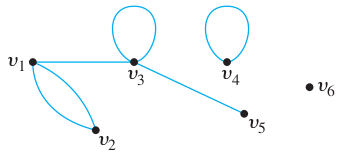
\includegraphics[scale=0.5]{../images/4.9.1.png}
\end{figure}

\begin{proof}
Total degree = 3+2+4+2+1 = 12, there are 6 edges (6 = 12/2).
\begin{center}
\arrayrulecolor{cyan}
\begin{tabular}{|c|c|c|c|c|c|c|}
\hline
{\bf vertex} & $v_1$ & $v_2$ & $v_3$ & $v_4$ & $v_5$ & $v_6$ \\
\hline
{\bf degree} & $3$ & $2$ & $4$ & $2$ & $1$ & $0$ \\
\hline
\end{tabular}
\arrayrulecolor{black}
\end{center}
\end{proof}

\subsection{Exercise 2}
\begin{figure}[ht!]
\centering
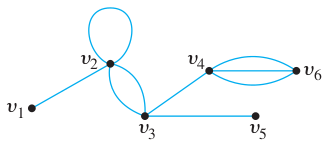
\includegraphics[scale=0.5]{../images/4.9.2.png}
\end{figure}

\begin{proof}
Total degree = 1+5+4+4+1+3 = 18, there are 9 edges (9 = 18/2).
\begin{center}
\arrayrulecolor{cyan}
\begin{tabular}{|c|c|c|c|c|c|c|}
\hline
{\bf vertex} & $v_1$ & $v_2$ & $v_3$ & $v_4$ & $v_5$ & $v_6$ \\
\hline
{\bf degree} & $1$ & $5$ & $4$ & $4$ & $1$ & $3$ \\
\hline
\end{tabular}
\arrayrulecolor{black}
\end{center}
\end{proof}

\subsection{Exercise 3}
A graph has vertices of degrees 0, 2, 2, 3, and 9. How many edges does the graph have?

\begin{proof}
The total degree of the graph is $0 + 2 + 2 + 3 + 9 = 16$, so, by the handshake theorem (Theorem 4.9.1), the number of edges is $16/2 = 8$.
\end{proof}

\subsection{Exercise 4}
A graph has vertices of degrees 1, 1, 4, 4, and 6.
How many edges does the graph have?

\begin{proof}
The total degree of the graph is $1 + 1 + 4 + 4 + 6 = 16$, so, by the handshake theorem (Theorem 4.9.1), the number of edges is $16/2 = 8$.
\end{proof}

{\bf \cy In each of $5-13$ either draw a graph with the specified properties or explain why no such graph exists.}

\subsection{Exercise 5}
Graph with five vertices of degrees 1, 2, 3, 3, and 5.

\begin{proof}
One such graph is
\begin{figure}[ht!]
\centering
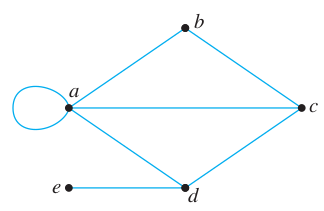
\includegraphics[scale=0.5]{../images/4.9.5.png}
\end{figure}
\end{proof}

\subsection{Exercise 6}
Graph with four vertices of degrees 1, 2, 3, and 3.

\begin{proof}
If there were a graph with four vertices of degree 1, 2, 3, and 3, then its total degree would be 9, which is odd. But by Corollary 4.9.2, the total degree of the graph must be even. {\it [This is a contradiction.]} Hence there is no such graph. (Alternatively, if there were such a graph, it would have an odd number of vertices of odd degree. But by Proposition 4.9.3 this is impossible.)
\end{proof}

\subsection{Exercise 7}
Graph with four vertices of degrees 1, 1, 1, and 4.

\begin{proof}
If there were a graph with four vertices of degree 1, 1, 1, and 4, then its total degree would be 7, which is odd. But by Corollary 4.9.2, the total degree of the graph must be even. {\it [This is a contradiction.]} Hence there is no such graph. (Alternatively, if there were such a graph, it would have an odd number of vertices of odd degree. But by Proposition 4.9.3 this is impossible.)
\end{proof}

\subsection{Exercise 8}
Graph with four vertices of degrees 1, 2, 3, and 4.

\begin{proof}
The graph given in Example 4.9.1 satisfies this (parallel edges and self-loops are required to make this happen):
\begin{figure}[ht!]
\centering
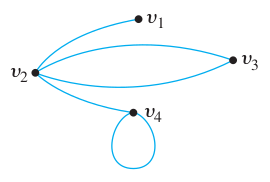
\includegraphics[scale=0.5]{../images/4.9.8.png}
\end{figure}
\end{proof}

\subsection{Exercise 9}
Simple graph with four vertices of degrees 1, 2, 3, and 4.

\begin{proof}
Suppose there were a simple graph with four vertices of degrees 1, 2, 3, and 4. Then the vertex of degree 4 would have to be connected by edges to four distinct vertices other than itself because of the assumption that the graph is simple (and hence has no loops or parallel edges). This contradicts the assumption that the graph has four vertices in total. Hence there is no simple graph with four vertices of degrees 1, 2, 3, and 4.
\end{proof}

\subsection{Exercise 10}
Simple graph with five vertices of degrees 2, 3, 3, 3, and 5.

\begin{proof}
Similar to Exercise 10, since the graph in question is simple and has 5 vertices, the maximum degree of any vertex is $5 - 1 = 4$, contradicting the fact that a vertex of degree 5 exists. So, such a graph does not exist.
\end{proof}

\subsection{Exercise 11}
Simple graph with five vertices of degrees 1, 1, 1, 2, and 3.
\begin{proof}
\begin{figure}[ht!]
\centering
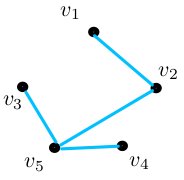
\includegraphics[scale=0.5]{../images/4.9.11.png}
\end{figure}
\end{proof}

\subsection{Exercise 12}
Simple graph with six edges and all vertices of degree 3.

\begin{proof}
\begin{figure}[ht!]
\centering
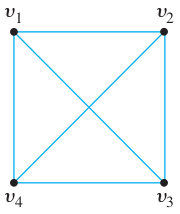
\includegraphics[scale=0.5]{../images/4.9.12.png}
\end{figure}
\end{proof}

\subsection{Exercise 13}
Simple graph with nine edges and all vertices of degree 3.

\begin{proof}
Since there are 9 edges, the total degree of such a graph has to be $9 \cdot 2 = 18$. Since all vertices have degree 3, there are $18 / 3 = 6$ vertices.
\begin{figure}[ht!]
\centering
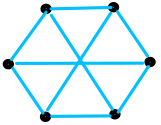
\includegraphics[scale=0.5]{../images/4.9.13.png}
\end{figure}
\end{proof}

\subsection{Exercise 14}
At a party attended by a group of people, two people knew one other person before the party, and five people knew two other people before the party. The rest of the people knew three other people before the party. A total of 15 pairs of people knew each other before the party.

\subsubsection{(a)}
How many people attending the party knew three other people before the party?

\begin{proof}
Define a graph $G$ by letting each vertex represent a person at the party and drawing an edge between each pair of people who knew each other before the party. Let $x$ be the number of people who knew three other people before the party. Then the total degree of the graph $ = 2\cdot 1 + 5\cdot 2 + x\cdot 3 = 12 + 3x$ because 2 people knew 1 other person before the party, 5 people knew 2 other people before the party, and $x$ people knew 3 other people before the party. 

In addition, since a total of 15 pairs of people knew each other before the party, the graph has 15 edges. By the handshake theorem (Theorem 4.9.1), the total degree is twice the number of edges. Hence the total degree of the graph $= 2 \cdot 15 = 30$. It follows that $12 + 3x = 30$. Thus $3x = 30 - 12 = 18$, and so $x = \frac{18}{3} = 6$. In other words, 6 people at the party knew 3 other people before the party.
\end{proof}

\subsubsection{(b)}
How many people attended the party?

\begin{proof}
Now the total number of people at the party is the sum of the number who knew 1 other person before the party, plus the number who knew 2 other people before the party, plus the number who knew 3 other people before the party. Therefore, the number of people at the party $= 2 + 5 + 6 = 13$.
\end{proof}

\subsection{Exercise 15}
A small social network contains three people who network friends with six other people in the network, one person who is network friend with five other people in the network, and five people who are network friends with four other people in the network. The rest are network friends with three other people in the network. The network contains 41 pairs of network friends.

\subsubsection{(a)}
How many people are network friends with three other people in the network?

\begin{proof}
Similar to Exercise 14, define a graph $G$ where vertices are people and edges represent networking relations. This is a simple graph (no self-loops: people do not ``network with themselves'' but only with other people, and no parallel edges: two people only network with each other once). So the number of people that a person networks with represents the degree of the vertex for that person. Now we can translate from English to math:

There are 3 people who network with 6 other people: in other words there are 3 vertices of degree 6. Similarly, one vertex of degree 5, 5 vertices of degree 4, and say $x$ vertices of degree 3 (let $x$ be the number of people who are network friends with 3 other people). And there are a total of 41 edges.

The total degree is $42 \cdot 2 = 82$. Counted the other way, the total degree is: $3 \cdot 6 + 1 \cdot 5 + 5 \cdot 4 + 3x = 43+3x$. So $82 = 43+3x$, therefore $39 = 3x$ so $x = 13$. So 13 people are network friends with three other people in the network.
\end{proof}

\subsubsection{(b)}
How many people are in the network?

\begin{proof}
$4 + 1 + 5 + 13 = 23$ people.
\end{proof}

\subsection{Exercise 16}
\subsubsection{(a)}
In a group of 15 people, is it possible for each person to have exactly 3 friends? Justify your answer. (Assume that friendship is a symmetric relationship: If $x$ is a friend of $y$, then $y$ is a friend of $x$.)

\begin{proof}
Suppose that, in a group of 15 people, each person had exactly three friends. Then you could draw a graph representing each person by a vertex and connecting two vertices by an edge if the corresponding people were friends. But such a graph would have 15 vertices, each of degree 3, for a total degree of 45. This would contradict the fact that the total degree of any graph is even. Hence the supposition must be false, and in a group of 15 people it is not possible for each to have exactly three friends.
\end{proof}

\subsubsection{(b)}
In a group of 4 people, is it possible for each person to have exactly 3 friends? Justify your answer.

\begin{proof}
Yes. Let each person in a group of 4 be friends with the other 3. Then each person has exactly 3 friends. This corresponds to the complete graph $K_{4}$:
\begin{figure}[ht!]
\centering
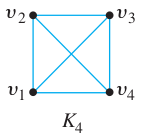
\includegraphics[scale=0.5]{../images/4.9.16.b.png}
\end{figure}
\end{proof}

\subsection{Exercise 17}
In a group of 25 people, is it possible for each to shake hands with exactly 3 other people? Justify your answer.

\begin{proof}
If we represent this as a graph, letting vertices represent people, and edges represent handshakes between people, then we would have a total degree of $25 \cdot 3 = 75$, which is odd, which is impossible by Corollary 4.9.2.
\end{proof}

\subsection{Exercise 18}
Is there a simple graph, each of whose vertices has even degree? Justify your answer.

\begin{proof}
Yes, for example $K_3$ (a triangle) is a simple graph where each vertex has degree 2:
\begin{figure}[ht!]
\centering
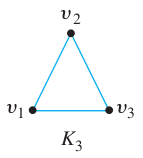
\includegraphics[scale=0.5]{../images/4.9.18.png}
\end{figure}
\end{proof}

\subsection{Exercise 19}
Suppose that $G$ is a graph with $v$ vertices and $e$ edges and that the degree of each vertex is at least $d_{min}$ and at most $d_{max}$. Show that
\[
\frac{1}{2}d_{min}\cdot v \leq e \leq \frac{1}{2}d_{max}\cdot v
\]
{\it Hint:} Let $t$ be the total degree of the graph, let $d_{min}$ be the minimum degree of any vertex in $G$, and let $d_{max}$ be the maximum degree of any vertex in $G$.

\begin{proof}
Let $a_1, \ldots, a_v$ be the vertices of $G$. The total degree of all vertices is twice the number of edges, so
\[
2e = \text{deg}(a_1) + \text{deg}(a_2) + \ldots + \text{deg}(a_v).
\]
We are given that for all $i = 1, 2, \ldots, v$, $d_{min} \leq \text{deg}(a_i) \leq d_{max}$. Therefore
\[
d_{min} \cdot v = d_{min} + d_{min} + \ldots + d_{min} \leq \text{deg}(a_1) + \text{deg}(a_2) + \ldots + \text{deg}(a_v)
\]
and
\[
\text{deg}(a_1) + \text{deg}(a_2) + \ldots + \text{deg}(a_v) \leq d_{max} + d_{max} + \ldots + d_{max} = d_{max} \cdot v.
\]
Combining we get $d_{min} \cdot v \leq 2e \leq d_{max} \cdot v$ and dividing by 2 we get the desired result.
\end{proof}

\subsection{Exercise 20}
\subsubsection{(a)}
Draw $K_6$, a complete graph on six vertices.

\begin{proof}
\begin{figure}[ht!]
\centering
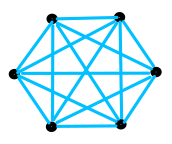
\includegraphics[scale=0.5]{../images/4.9.20.png}
\end{figure}
\end{proof}

\subsubsection{(b)}
Use the result of Example 4.9.9 to show that the number of edges of a simple graph with $n$ vertices is less than or equal to $\frac{n(n - 1)}{2}$.

\begin{proof}
By the result of Example 4.9.9, the number of edges of $K_n$ is $\frac{n(n - 1)}{2}$.

If $G$ is any simple graph with $n$ vertices, then $G$ can have at most as many edges as $K_n$ does, because $K_n$ is complete, and $G$ may be complete (in which case it would have the same number of edges as $K_n$) or incomplete (in which case it would have fewer edges than $K_n$).

Therefore the number of edges of a simple graph with $n$ vertices is less than or equal to $\frac{n(n - 1)}{2}$.
\end{proof}

\subsection{Exercise 21}

\subsubsection{(a)}
In a simple graph, must every vertex have degree that is less than the number of vertices in the graph? Why?

\begin{proof}
Yes. Let $G$ be a simple graph with $n$ vertices and let $v$ be a vertex of $G$. Since G has no parallel edges, $v$ can be joined by at most a single edge to each of the $n - 1$ other vertices of $G$, and since $G$ has no loops, $v$ cannot be joined to itself. Therefore, the maximum degree of $v$ is $n - 1$.
\end{proof}

\subsubsection{(b)}
Can there be a simple graph that has four vertices all of different degrees? Why?

\begin{proof}
No. Suppose there is a simple graph with four vertices, all of which have different degrees. By part (a), no vertex can have degree greater than three, and of course, no vertex can have degree less than 0. Therefore, the only possible degrees of the vertices are 0, 1, 2, and 3. Since all four vertices have different degrees, there is one vertex with each degree. But then the vertex of degree 3 is connected to all the other vertices, which contradicts the fact that one of the vertices has degree 0. Hence the supposition is false, and there is no simple graph with four vertices each of which has a different degree.
\end{proof}

\subsubsection{(c)}
For any integer $n \geq 5$, can there be a simple graph that has $n$ vertices all of different degrees? Why?

\begin{proof}
No. In a simple graph that has $n$ vertices, the maximum degree of a vertex is $n-1$ by part (a). So, if $n$ vertices in a simple graph all have different degrees, then these degrees must be $0, 1, 2, \ldots, n-1$. So there is a vertex $v$ such that deg$(v) = 0$. But the vertex with degree $n-1$ is connected to every other vertex, including $v$. So deg$(v) \geq 1$, contradicting deg$(v) = 0$. Thus such a simple graph is impossible.
\end{proof}

\subsection{Exercise 22}
In a group of two or more people, must there always be at least two people who are acquainted with the same number of people within the group? Why?

{\it Hint:} Use the result of exercise 21, part (c).

\begin{proof}
Yes. If we represent people with vertices and acquaintances with edges, we obtain a simple graph: no person is counted as being ``acquainted with themselves'' but only with others, so there are no self-loops; and if two people are acquainted, then only one edge is enough to represent this (it is only counted once), so there are no parallel edges.
By Exercise 21 part (c), it is impossible for all vertices in a simple graph to have different degrees. Therefore there are at least two people who are acquainted with t he same number of people within the group.
\end{proof}

\subsection{Exercise 23}
Recall that $K_{m,n}$ denotes a complete bipartite graph on $(m, n)$ vertices.

\subsubsection{(a)}
Draw $K_{4,2}$.

\begin{proof}
\begin{figure}[ht!]
\centering
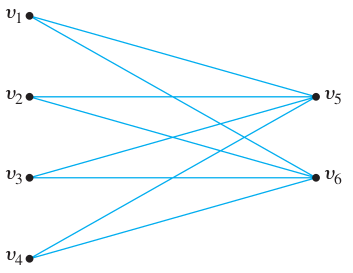
\includegraphics[scale=0.4]{../images/4.9.23.a.png}
\end{figure}
\end{proof}

\subsubsection{(b)}
Draw $K_{1,3}$.

\begin{proof}
\begin{figure}[ht!]
\centering

\includegraphics[scale=0.5]{../images/4.9.23.b.png}
\end{figure}
\end{proof}

\subsubsection{(c)}
Draw $K_{3,4}$.

\begin{proof}
\begin{figure}[ht!]
\centering

\includegraphics[scale=0.5]{../images/4.9.23.c.png}
\end{figure}
\end{proof}

\subsubsection{(d)}
How many vertices of $K_{m,n}$ have degree $m$? degree $n$?

\begin{proof}
If $n \neq m$, the vertices of $K_{m,n}$ are divided into two groups: one of size $m$ and the other of size $n$. Every vertex in the group of size $m$ has degree $n$ because each is connected to every vertex in the group of size $n$. So $K_{m,n}$ has $m$ vertices of degree $n$. Similarly, every vertex in the group of size $n$ has degree $m$ because each is connected to every vertex in the group of size $m$. So $K_{m,n}$ has $n$ vertices of degree $m$. Note that if $n = m$, then all $n + m = 2n$ vertices have the same degree, namely, $n$.
\end{proof}

\subsubsection{(e)}
What is the total degree of $K_{m,n}$?

\begin{proof}
By part (d), the group of $m$ vertices each have degree $n$, so they contribute a total of $mn$ degrees; and the group of $n$ vertices each have degree $m$, so they contribute a total of $nm$ degrees. So the total degree overall is $2mn$.
\end{proof}

\subsubsection{(f)}
Find a formula in terms of $m$ and $n$ for the number of edges of $K_{m,n}$. Justify your answer.

\begin{proof}
Since the total degree is equal to twice the number of edges, $e = 2mn / 2 = mn$.
\end{proof}

\subsection{Exercise 24}
\begin{figure}[ht!]
\centering
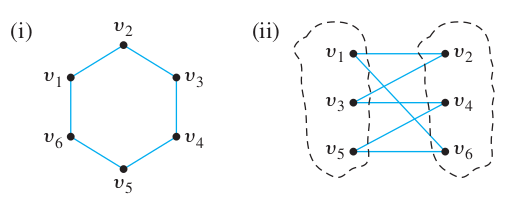
\includegraphics[scale=0.5]{../images/4.9.24.1.png}
\end{figure}

A (general) bipartite graph G is a simple graph whose vertex set can be partitioned into two disjoint nonempty subsets $V_1$ and $V_2$ such that vertices in $V_1$ may be connected to vertices in $V_2$, but no vertices in $V_1$ are connected to other vertices in $V_1$ and no vertices in $V_2$ are connected to other vertices in $V_2$. For example, the bipartite graph $G$ illustrated in (i) can be redrawn as shown in (ii). From the drawing in (ii), you can see that $G$ is bipartite with mutually disjoint vertex sets $V_1 = \{v_1, v_3, v_5\}$ and $V_2 = \{v_2, v_4, v_6\}$.

Find which of the following graphs are bipartite. Redraw the bipartite graphs so that their bipartite nature is evident.

\begin{figure}[ht!]
\centering
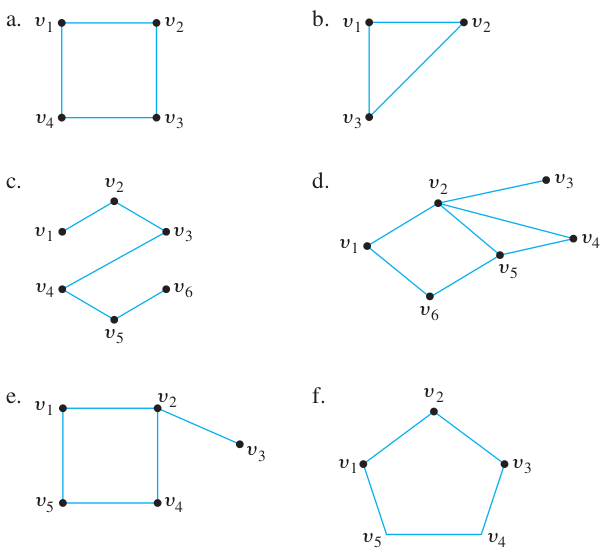
\includegraphics[scale=0.5]{../images/4.9.24.2.png}
\end{figure}

\subsubsection{(a)}
Graph a. above

\begin{proof}
\begin{figure}[ht!]
\centering
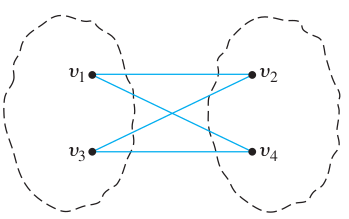
\includegraphics[scale=0.4]{../images/4.9.24.a.png}
\end{figure}
\end{proof}

\subsubsection{(b)}
Graph b. above

\begin{proof}
Suppose this graph is a bipartite. Then the vertex set can be partitioned into two mutually disjoint subsets such that vertices in each subset are connected by edges only to vertices in the other subset and not to vertices in the same subset. Now $v_1$ is in one subset of the partition, say, $V_1$. Since $v_1$ is connected by edges to $v_2$ and $v_3$ both $v_2$ and $v_3$ must be in the other subset, $V_2$. But $v_2$ and $v_3$ are connected by an edge to each other. This contradicts the fact that no vertices in $V_2$ are connected by edges to other vertices in $V_2$. Hence the supposition is false, and so the graph is not bipartite.
\end{proof}

\subsubsection{(c)}
Graph c. above

\begin{proof}
\begin{figure}[ht!]
\centering
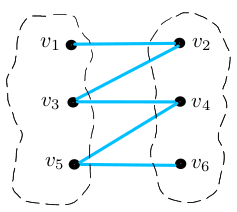
\includegraphics[scale=0.4]{../images/4.9.24.c.png}
\end{figure}
\end{proof}

\subsubsection{(d)}
Graph d. above

\begin{proof}
This graph is not bipartite due to the triangle formed by $v_2, v_4, v_5$. Argue by contradiction and assume it is bipartite, with disjoint vertex sets $V_1, V_2$. Then either $v_2 \in V_1$ or $v_2 \in V_2$. If $v_2 \in V_1$, then since $v_2$ is connected to both $v_4$ and $v_5$, we must have $v_4 \in V_2$ and $v_5 \in V_2$. But $v_4$ and $v_5$ are also connected, contradicting the definition of bipartite. Similarly if $v_2 \in V_2$ then $v_4 \in V_1$ and $v_5 \in V_1$ and we get a similar contradiction. Therefore the graph is not bipartite.
\end{proof}

\subsubsection{(e)}
Graph e. above

\begin{proof}
\begin{figure}[ht!]
\centering
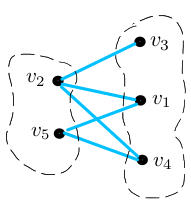
\includegraphics[scale=0.4]{../images/4.9.24.e.png}
\end{figure}
\end{proof}

\subsubsection{(f)}
Graph f. above

\begin{proof}
This graph is not bipartite. Argue by contradiction and assume it is bipartite, with disjoint vertex sets $V_1, V_2$. Then either $v_1 \in V_1$ or $v_1 \in V_2$. If $v_1 \in V_1$, then since $v_1$ is connected to both $v_2$ and $v_5$, we must have $v_2 \in V_2$ and $v_5 \in V_2$. So $v_3 \in V_1$ and $v_4 \in V_1$. But $v_3$ is connected to $v_4$, contradicting the definition of bipartite. Similarly if $v_1 \in V_2$ then $v_2 \in V_1$ and $v_5 \in V_1$ and $v_3 \in V_2$ and $v_4 \in V_2$ and we get a similar contradiction. Therefore the graph is not bipartite.
\end{proof}

\subsection{Exercise 25}
Suppose $r$ and $s$ are any positive integers. Does there exist a graph $G$ with the property that $G$ has vertices of degrees $r$ and $s$ and of no other degrees? Explain.

\begin{proof}
Yes. Let $G = K_{r,s}$. Then by the solution to Exercise 23 (d) every vertex has degree either $r$ or $s$.
\end{proof}

\section{Exercise Set 4.10}

\subsection{Exercise 1}

\begin{proof}

\end{proof}

\subsection{Exercise 2}

\begin{proof}

\end{proof}

\subsection{Exercise 3}

\subsubsection{(a)}

\begin{proof}

\end{proof}

\subsubsection{(b)}

\begin{proof}

\end{proof}

\subsection{Exercise 4}

\begin{proof}

\end{proof}

\subsection{Exercise 5}

\begin{proof}

\end{proof}

\subsection{Exercise 6}

\begin{proof}

\end{proof}

\subsection{Exercise 7}

\begin{proof}

\end{proof}

\subsection{Exercise 8}

\subsubsection{(a)}

\begin{proof}

\end{proof}

\subsubsection{(b)}

\begin{proof}

\end{proof}

\subsection{Exercise 9}

\begin{proof}

\end{proof}

\subsection{Exercise 10}

\begin{proof}

\end{proof}

\subsection{Exercise 11}

\begin{proof}

\end{proof}

\subsection{Exercise 12}

\begin{proof}

\end{proof}

\subsection{Exercise 13}

\begin{proof}

\end{proof}

\subsection{Exercise 14}

\begin{proof}

\end{proof}

\subsection{Exercise 15}

\begin{proof}

\end{proof}

\subsection{Exercise 16}

\begin{proof}

\end{proof}

\subsection{Exercise 17}

\begin{proof}

\end{proof}

\subsection{Exercise 18}

\begin{proof}

\end{proof}

\subsection{Exercise 19}

\begin{proof}

\end{proof}

\subsection{Exercise 20}

\begin{proof}

\end{proof}

\subsection{Exercise 21}

\begin{proof}

\end{proof}

\subsection{Exercise 22}

\begin{proof}

\end{proof}

\subsection{Exercise 23}

\subsubsection{(a)}

\begin{proof}

\end{proof}

\subsubsection{(b)}

\begin{proof}

\end{proof}

\subsection{Exercise 24}

\begin{proof}

\end{proof}

\subsection{Exercise 25}

\subsubsection{(a)}

\begin{proof}

\end{proof}

\subsubsection{(b)}

\begin{proof}

\end{proof}

\subsection{Exercise 26}

\subsubsection{(a)}

\begin{proof}

\end{proof}

\subsubsection{(b)}

\begin{proof}

\end{proof}

\subsection{Exercise 27}

\subsubsection{(a)}

\begin{proof}

\end{proof}

\subsubsection{(b)}

\begin{proof}

\end{proof}

\subsubsection{(c)}

\begin{proof}

\end{proof}

\subsection{Exercise 28}

\subsubsection{(a)}

\begin{proof}

\end{proof}

\subsubsection{(b)}

\begin{proof}

\end{proof}

\subsubsection{(c)}

\begin{proof}

\end{proof}

\subsection{Exercise 29}

\begin{proof}

\end{proof}

\subsection{Exercise 30}

\begin{proof}

\end{proof}

\subsection{Exercise 31}

\begin{proof}

\end{proof}

\subsection{Exercise 32}

\begin{proof}

\end{proof}

\end{document}
